%%%%%%%%%%%%%%%%%%%%%%%% DOCUMENTCLASS %%%%%%%%%%%%%%%%%%%%%%%%

\documentclass[a4paper,12pt]{report}

%%%%%%%%%%%%%%%%%%%%%%%% PACKAGES %%%%%%%%%%%%%%%%%%%%%%%%

\usepackage[utf8]{inputenc}
\usepackage[spanish, es-tabla]{babel}
\usepackage{anysize}
\usepackage{titlesec} % Para customizar títulos entiendo que es (template darío)
\usepackage{setspace} % Para setear el espacio entre lineas (template darío)

\usepackage[draft]
{graphicx} % Draft hace que no se redeneé la imagen al compilar entonces compilar x1000 más rápido. Ta buenardo (template darío)
\usepackage{float}

\usepackage{afterpage} % Entiendo que con este package y usando el comando \afterpage{\clearpage} cuando te queda una figura muy arriba sin texto abajo y media hoja vacía, te completa el espacio con texto. Está bueno porque latex se chotea seguido en ese sentido.

\usepackage{amsmath,amssymb}
\usepackage{xcolor} % 14/12/2021 texto en color

\usepackage{enumerate} % template dario
\usepackage{lscape} % rota la hoja si por ejemplo hay una tabla o figura muy grande/larga (dudo usarlo) (template darío)
\usepackage{verbatim} % (template darío)
\usepackage{appendix} % (template darío)
\usepackage{array} % (template darío)
\usepackage{physics}

\usepackage{multirow}
\usepackage{multicol}

\usepackage[font=small]{caption} %10/3/2022 para achicar el tamaño de las palabras "Fig" o "Tabla" en los captions
\usepackage{subcaption}
\usepackage{fancybox}
\usepackage{letltxmacro}

\usepackage{xargs}
\usepackage[hidelinks]{hyperref}
% (citas)
\usepackage[superscript,biblabel,nomove]{cite}
% (citas) hace las citas superíndices

\usepackage{mathtools} % 02/02/2022 para tener el prescript{}{} índice y supraíndice del lado izq a misma altura
\usepackage{mathrsfs} %03/02/2022 Para la L del lagrangiano bien cheta 14/10/2021

\usepackage{titlesec}% http://ctan.org/pkg/titlesec
\usepackage{fancyhdr}

\usepackage{siunitx} %03/01/2022 <- Para unidades

\usepackage{enumitem,kantlipsum} %05/01/2022 <- para indentar dentro del enumerate

\usepackage{booktabs} %13/01/2022 Para tener tablas de libros
\usepackage{scalerel} %20/03/2022 Para escalar tamaños de fuentes en ecuaciones


%%%%%%%%%%%%%%%%%%%%%%%% NEW COMMANDS %%%%%%%%%%%%%%%%%%%%%%%%
\makeatletter 
\renewcommand{\@citess}[1]{\textsuperscript{\,[#1]}}

\newcommand{\eh}{e\mbox{-}h} % 03/01/2022 <- mi forma de escribir la energía de creación electrón hueco

% 03/02/2022 Command for a cheta L for the lagrangian partir 
\newcommand{\Lagr}{\mathscr{L}}

% (raiz) Para hacer la raiz cuadrada con el cierre al final
\makeatletter
\let\oldr@@t\r@@t
\def\r@@t#1#2%
    {%
        \setbox0=\hbox{$\oldr@@t#1{#2\,}$}\dimen0=\ht0
        \advance\dimen0-0.2\ht0
        \setbox2=\hbox{\vrule height\ht0 depth -\dimen0}%
        {\box0\lower0.4pt\box2}%
    }
\LetLtxMacro{\oldsqrt}{\sqrt}
\renewcommand*{\sqrt}[2][\ ]{\oldsqrt[#1]{#2}}
\makeatother
% (raiz) nacho: 31/03/2018 17:35

%%%%%%%%%%%%%%%%%%%%%%%% MODIFICACIONES %%%%%%%%%%%%%%%%%%%%%%%%

% modifican el nombre que muestra3
\addto\captionsspanish{\renewcommand*\contentsname{Índice}}
\addto\captionsspanish{\renewcommand*{\bibname}{Referencias}} % cambia el nombre de la 'Bibliografía' por 'Referencias'

%\titleformat{\chapter}[hang]{\bfseries\Large}{\thechapter.}{12pt}{\bfseries\Large} % tamaño de la letra de chapter. Queda igual que la de section. No sé si me gusta
%\titleformat{\section}[hang]{\bfseries\large}{\thesection}{12pt}{\bfseries\large}


%%%%%%%%%%%%%%%%%%%%%%%% SETEOS %%%%%%%%%%%%%%%%%%%%%%%%

%\setlength{\parskip}{1em} % Por lo que vi, me genera un espaciado en el índice (no me gusta como queda 3jj3j3, negociar) (template darío)

%\setlength{\parindent}{10pt} % modifica la indentación (10 pt es menos que la por defecto y no sé si me gusta. Negociar)


\pagestyle{fancy}
\lhead{{}}
%%% Dario: Te gusta como queda lo que hace la linea anterior? aparece tu nombre en todas las hojas, es medio mucho no? no lo vi en otras tesis creo. Me gusta más que aparezca el nombre de la sección en la que estas, que es lo que hace si lo dejas comentado.
%\fancyhead[L]{\nouppercase{\slshape \leftmark}} % Parte izquierda del encabezado
%\fancyhead[C]{\nouppercase{\slshape \leftmark}} % Medio del encabezado
\fancyhead[R]{\nouppercase{\slshape \leftmark}} % Parte derecha del encabezado

\setlength{\headheight}{16pt} %Soluciona el warning de " fancyhdr \headheight is to small. use at least 14.9999 o algo así decía << No de nuevo decía >>

\marginsize{2cm}{2cm}{2cm}{2cm}
\renewcommand{\baselinestretch}{1.3} % separa los renglones

\title{\textbf{\Huge Propiedades de los sensores de silicio más allá del ruido de lectura}}
\author{Ignacio Martín Gómez Florenciano}

%\date{Abril 2022}
\date{
\bigskip
\parbox{\linewidth}
    {\centering%
        \endgraf
        \bigskip
        \vspace{8cm}
            Tesis de Licenciatura en Ciencias Físicas
        \endgraf
        \bigskip
            Facultad de Ciencias Exactas y Naturales
        \endgraf
        \bigskip
            Universidad de Buenos Aires
        \endgraf
        \vspace{2cm}
    }
Mayo 2022
\newpage
\thispagestyle{empty} \mbox{}
\thispagestyle{empty}
}

\begin{document}
    
    \maketitle

    %%%%%%%%%%%%  segunda pagina %%%%%%%%%%%%%%%%%%%%%%%%%%%%%%%%%%
\thispagestyle{empty}
\noindent TEMA: Propiedades de los sensores de silicio más allá del ruido de lectura.\\
\\
\noindent ALUMNO: L.U. N$^\circ\ 116/13$\\
\\
\noindent LUGAR DE TRABAJO: Facultad de Ciencias Exactas y Naturales - Universidad de Buenos Aires\\
\\
\noindent DIRECTOR: Dr. Darío P. Rodrigues F. Maltéz\\
\\
\noindent CODIRECTOR: \\
\\
\noindent FECHA DE INICIACIÓN: Marzo 2021\\
\\
\noindent FECHA DE FINALIZACIÓN:  Abril 2022\\
\\
\noindent FECHA DE EXAMEN: No sé\\
\\
\noindent INFORME FINAL APROBADO POR:\\
\vfill
\begin{multicols}{2}    
\rule[0pt]{2.5in}{0.5pt}\\
Autor: Ignacio M. Gómez Florenciano
\vspace{3em}

\rule[0pt]{2.5in}{0.5pt}\\
Director: Dr. Dario Rodrigues
\vspace{3em}
   
\rule[0pt]{2.5in}{0.5pt}\\
Profesora de Tesis de Licenciatura
    
\columnbreak
\rule[0pt]{2.5in}{0.5pt}\\
Jurado 
\vspace{3em}
    
\rule[0pt]{2.5in}{0.5pt}\\
Jurado 
\vspace{3em}
    
\rule[0pt]{2.5in}{0.5pt}\\
Jurado 
\end{multicols}  
%------PÁGINA VACIA ------------------
\newpage
\thispagestyle{empty} \mbox{}
\thispagestyle{empty}
%%%%%%% fin segunda hoja %%%%%%%%%%%%%%%%%%%%%%%%%%%%%%%%%%%%%
    
     %%%%%%%%%%%%%%%%%%%%%%%%%%%%%%%% AGRADECIMIENTOS %%%%%%%%%%%%%%%%%%%%%%%%%%%%%%%%
\newpage
\thispagestyle{empty}
 \vspace*{150pt}
\begin{flushright}
\textit{A mis viejos}
\end{flushright}
%------PÁGINA VACIA ------------------
\newpage
\thispagestyle{empty} \mbox{}
\thispagestyle{empty}
 %%%%%%%%%%%%%%%%%%%%%%%%%%%%%%%% FIN AGRADECIMIENTOS %%%%%%%%%%%%%%%%%%%%%%%%%%%%%%%%

	\newpage
%\begin{center}
%    {\Large \textbf{Resumen}}
%\end{center}
\chapter*{Resumen}
\thispagestyle{empty}
%<<Breve introducción>>
\noindent El ruido de lectura en los sensores CCDs ha sido una limitación inherente a la electrónica de estos dispositivos, imponiendo límites en la resolución con que podía medirse la carga en ellos generada. Los sensores \textit{Skipper}-CCDs, por su parte, han logrado superar esta barrera, reduciendo el ruido de lectura a niveles subelectrónicos. Sin embargo, el ruido de lectura no es el único factor que está en juego al momento de procesar mediciones realizadas con este tipo de sensores: los eventos provenientes de fuentes que no son de interés y los inducidos por fenómenos intrínsecos a la naturaleza de las interacciones, deben ser también considerados.


%\textbf{<<Objetivo de la tesis>>}
En esta tesis se estudió el fondo presente en un conjunto de más de $900$ imágenes tomadas con un sensor \textit{Skipper}-CCD, de forma de caracterizarlo con precisión en sus valores medios. A su vez se probaron tres diferentes umbrales de detección de eventos, de forma tal de elegir aquel que aumente lo más posible la estadística introduciendo el menor sesgo posible en los datos. Una vez logrado esto, se utilizó la información obtenida de los análisis para corregir los sesgos presentes en la determinación del factor de Fano y la energía de creación electrón-hueco, junto con un modelo de ajuste de los datos, especialmente diseñado para reproducir los efectos introducidos por el detector.


%\textbf{<<Trabajo realizado>>}
En paralelo, se estudió el fenómeno de ionización por medio de simulaciones Monte Carlo. Para ello se partió de un modelo muy sencillo para luego adoptar uno más sofisticado, con el fin de poner en evidencia las razones por las cuales el factor de Fano medido experimentalmente es un orden de magnitud menor a la unidad. De estas simulaciones se obtuvieron resultados para el factor de Fano semejantes a los obtenidos experimentalmente.


%\textbf{<<Resultados>>}
Los resultados de este trabajo presentan la determinación de las magnitudes antes mencionadas para un rango de energías inaccesible hasta el momento, lo cual es de vital importancia en la caracterización de estos dispositivos en el rango de bajas energías, donde los CCDs convencionales presentan importantes barreras debido al ruido de lectura. Es por esto que la importancia de este trabajo radica en la combinación de la tecnología \textit{Skipper} con el uso de técnicas de análisis que permitieron corregir sesgos en mediciones que, hasta el momento, no habían podido realizarse.


%\textbf{<<Perspectivas a futuro?>>}
%------PÁGINA VACIA ------------------
\newpage
\thispagestyle{empty} \mbox{}
\thispagestyle{empty}
%-------------------------------
    
    \newpage
\pagenumbering{roman} %numero de pagina en números romanos
\setcounter{page}{1}  %comienza a contar desde 1

\tableofcontents

\newpage
\thispagestyle{empty} \mbox{}
\thispagestyle{empty}

    \newpage
\pagenumbering{arabic}  %numero de pagina numeración arábiga
\setcounter{page}{1}    %comienza a contar desde 1

\chapter{Introducción}
\noindent Dependiendo de la energía de la radiación incidente en los sensores, esta puede ser capaz de ionizar electrones del Si.  
La relación entre la carga producida y la energía incidente, es decir la energía necesaria para producir un par electrón-hueco, resulta ser de fundamental importancia para traducir espectros de carga en espectros de energía.

Por otro lado, existen diferentes fenómenos que modifican la forma de los espectros de carga producidos por la radiación incidente en los sensores. Entre ellos, los dos más importantes son: el factor de Fano, que cuantifica la dispersión de carga; y las deficiencias en la colección de carga, que tienden a producir colas hacia bajas energías en los picos producidos por radiación monoenergética.

En este capítulo se describen tres cantidades que describen tanto propiedades del silicio como del sensor, y que en el marco de esta tesis han sido estudiadas mas allá del ruido de lectura gracias a la tecnología Skipper-CCD.

%%%%%%%%%%%%%%%%%%%%%%%%%%%%%%%%%%%%%%%%%%%%%%%%%%%%%%%%%%%%%%%%%%
%%%%%%%%%%%%%%%%%%%%%%%%%%%%%%%%%%%%%%%%%%%%%%%%%%%%%%%%%%%%%%%%%%
\section{Factor de Fano y energía de creación electrón-hueco}
\noindent El factor de Fano mide la relación entre la dispersión de una distribución de carga producida en un detector y su media. Viene dado por
\begin{equation*}
    F = \frac{\sigma^{2}}{\mu}
\end{equation*}
donde $\sigma^{2}$ es la varianza de la distribución de carga y $\mu$ es la media. 
Para el caso particular de una distribución de Poisson, la varianza y la esperanza coinciden, de forma que el factor de Fano equivale a $1$. 
Estas distribuciones de carga son el producto de la interacción de fotones con el detector, que depositan energía en el material ionizando cargas que a su vez ionizan a otras a su paso. 
%\textcolor{red}{ASI PARECIERA QUE LOS FOTONES SON QUIENES IONIZAN A SU PASO, PERO EN REALIDAD SON LOS ELECTRONES QUE GANARON ENERGIA DE ESOS FOTONES, ARREGLAR.}

Dicha distribución tiene origen en que la energía transferida en cada interacción no es constante y, por lo tanto, para una dada energía inicial de la partícula incidente, tampoco será constante el número de cargas generadas.

Por otro lado, la energía de creación electrón-hueco $\varepsilon_{\eh}$ es medida en valor medio, ya que es calculada a través del cociente entre la energía entregada al detector y la carga en él producida. 
Si bien $\varepsilon_{\eh}$ está relacionada con la energía del \textit{band gap} del silicio (entre la banda de valencia y la banda de conducción, $E_{g}\sim 1.1\,\si{eV}$\cite{Janesick}), debido a que durante el proceso de interacción parte de la energía entregada al material puede disiparse como fonones, la energía de creación electrón-hueco resulta ser mayor, en promedio, que la energía del \textit{gap}.

La estimación precisa de ambas magnitudes es de vital importancia en la caracterización de este tipo de detectores, debido a que, por ejemplo, parámetros como la eficiencia cuántica dependen fuertemente de ellos. Además es importante determinar la dependencia de estas magnitudes con la energía ya que, en particular, el factor de Fano a energías por debajo de $1\,\si{keV}$ es clave para el cálculo de sensibilidad en experimentos de búsqueda de materia oscura liviana, como es caso del experimento SENSEI (\textit{Sub-Electron Noise Skipper-CCD Experiment Instrument})\cite{barak} e interacciones de neutrinos dentro\cite{moroni1} y fuera del modelo estándar\cite{moroni2}.

%%%%%%%%%%%%%%%%%%%%%%%%%%%%%%%%%%%%%%%%%%%%%%%%%%%%%%%%%%%%%%%%%%
%%%%%%%%%%%%%%%%%%%%%%%%%%%%%%%%%%%%%%%%%%%%%%%%%%%%%%%%%%%%%%%%%%
\section{CCD y Skipper CCD}
\noindent Los dispositivos CCD (\textit{Charge Coupled Devices}) fueron inventados en 1969 en los Laboratorios Bell, por Willard Boyle y George Smith, en su búsqueda por fabricar dispositivos de memoria. Finalmente, los CCD's no fueron utilizados con este fin al ser superados por otras tecnologías, pero sí demostraron un gran potencial como sensores de luz y partículas. Tal es así que en el año 2010 sus inventores recibieron el premio Nobel de física\cite{Boyle, Smith}.

Estos dispositivos están hechos esencialmente de silicio y sus elementos constitutivos fundamentales son capacitores MOS (por \textit{metal-oxide-semiconductor}). Estos conforman los píxeles del detector, siendo por lo general millones y ocupando casi la totalidad de la superficie del sensor. Los capacitores MOS se componen generalmente de un sustrato semiconductor dopado, sobre el cual se deposita una delgada capa de óxido y a su vez sobre esta se coloca un metal de contacto. Este contacto metálico se encuentra a un voltaje $V_{G}$ y otro contacto debajo del semiconductor se encuentra a tierra. Dependiendo del valor de $V_{G}$ se obtienen distintos regímenes del MOS\cite{Chenming} donde, en particular, uno de ellos genera una región de depleción cerca del óxido, el cual permite acumular carga minoritaria. Un esquema de la vista lateral en corte de un capacitor MOS puede verse en la Figura \ref{fig:PixelCrossSection}.
\begin{figure}[h]
    \centering
        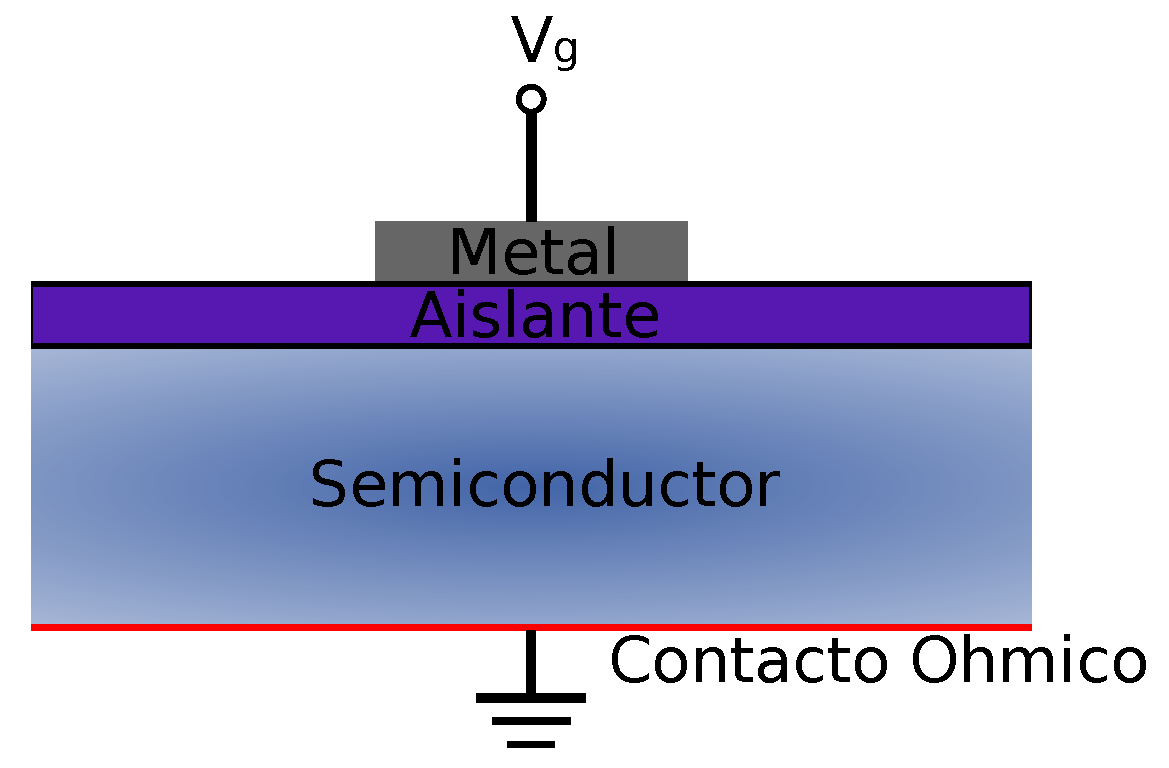
\includegraphics[scale=.35]{Figs/PixelCrossSection.pdf}
    \caption{Esquema de un corte lateral de un capacitor MOS (píxel).}
    \label{fig:PixelCrossSection}
\end{figure}
Además de los píxeles, como se puede ver en la Figura \ref{fig:ArgquitecturaCCDn}, los CCDs están compuestos de \textit{channel-stops} que se encargan de evitar que la carga de los píxeles migre entre columnas vecinas, mientras que los controladores verticales, con las señales $V_{1}$, $V_{2}$ y $V_{3}$, son las responsables de desplazarla secuencialmente de forma vertical. 
Otra parte fundamental de estos detectores es el registro horizontal, donde están los píxeles horizontales de la Figura \ref{fig:ArgquitecturaCCDn}, que es la región del CCD donde la carga es migrada de forma horizontal gracias a los estados $H_{1}$, $H_{2}$ y $H_{3}$ hacia el nodo de sensado.
\begin{figure}[h]
    \centering
        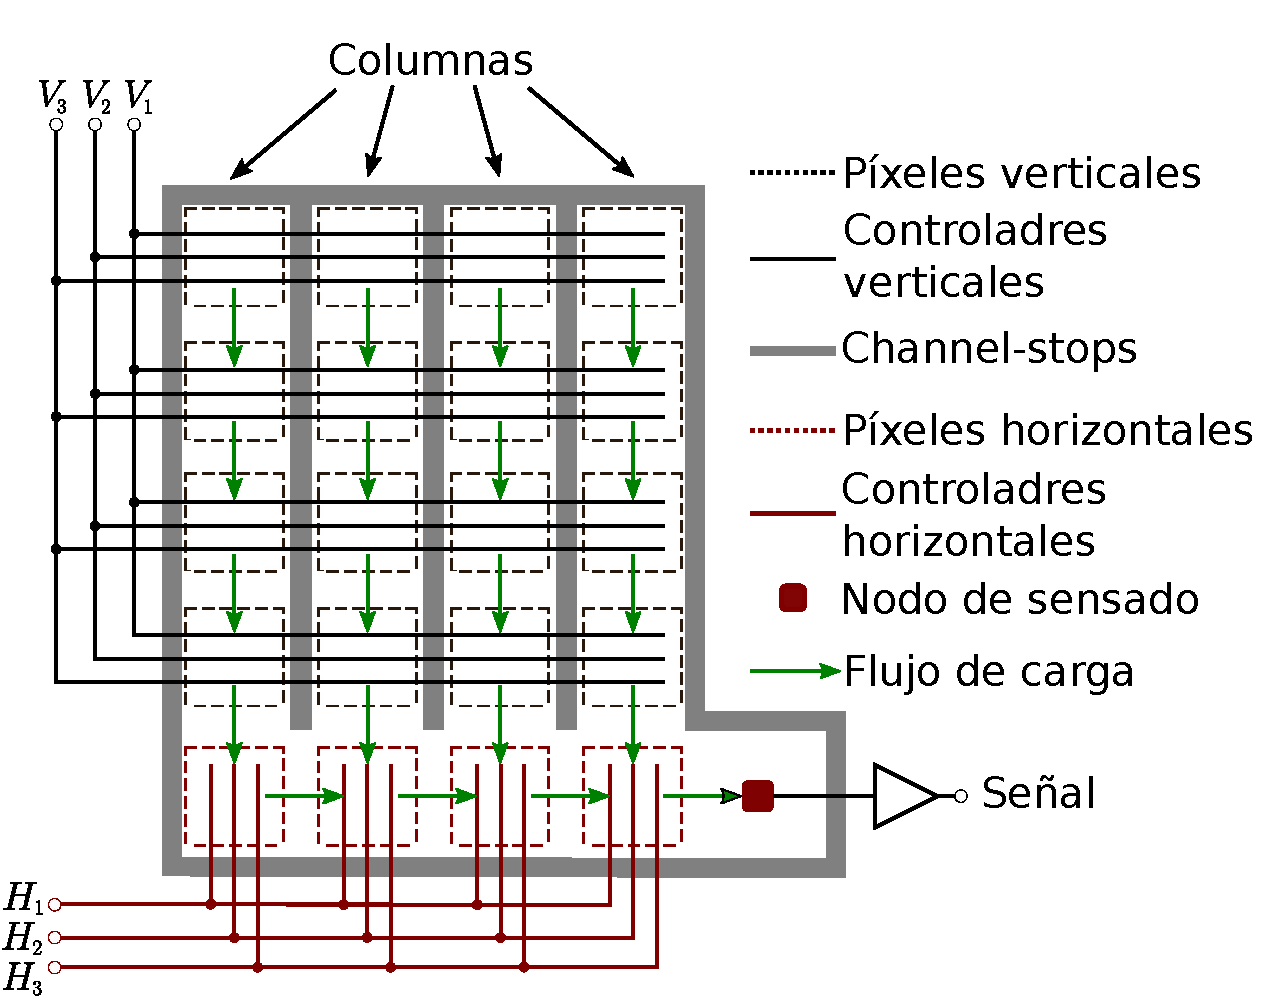
\includegraphics[scale=.5]{Figs/ArquitecturaCCD.pdf}
    \caption{Ilustración esquemática de un sensor CCD de $4\times4$ píxeles. Las flechas muestran la dirección en la que la carga es desplazada píxel a píxel para luego ser colectada por el nodo de sensado.}
    \label{fig:ArgquitecturaCCDn}
\end{figure}
El principio de operación de un CCD se puede dividir en cuatro etapas, que a grandes rasgos son:
\begin{itemize}
    \item Exposición del detector: el tiempo de exposición es variable y depende del tipo de medición que se desee utilizar. Durante la exposición, la radiación incidente interactúa con el detector, generalmente generando pares electrón-hueco. 
    \item Colección: los electrones son luego arrastrados por el campo eléctrico del detector presente en su volumen hacia los pozos de potencial de los píxeles donde son colectados.
    \item Transferencia: dado que la medición de la carga colectada en los píxeles se realiza de forma secuencial, la misma debe ser transferida de un píxel a otro.
    \item Medición de la carga: al llegar al nodo de sensado, un amplificador de salida cuantifica la carga.
\end{itemize}
Los CCD's convencionales son capaces de alcanzar ruidos de lectura del orden de los $2\,e^{-}\si{rms/pix}$, gracias a la técnica de muestreo doblemente correlacionado\cite{Tiffenberg}. Sin embargo, en aplicaciones de bajas energías, el ruido electrónico de lectura redunda en una barrera al límite de energías que pueden medirse con estos sensores manteniendo la precisión deseada. 

%\textcolor{red}{LO QUE SIGUE DICE "ESTAS CANTIDADES" PERO HACE RATO QUE NO SE HABLA DEL FACTOR DE FANO, PARECE RECORTADO DE OTRO LADO. ANTES DE PONER EL GRAFICO QUE SIGUE FALTA OTRO PARRAFO EXPLICANDO QUE EL RUIDO DE LECTURA TIENE IMPACTO EN LA MEDICION DE LAS CANTIDADES QUE SON DE INTERES EN ESTA TESIS}
Por debajo de los $2\,\si{keV}$ la contribución del ruido de lectura a la determinación del factor de Fano y la energía de creación electrón-hueco puede superar el $30\,\%$, como se esquematiza en la Figura \ref{fig:Fano_y_ruido}. Esto representa un impacto considerable en la determinación de estas cantidades que son de interés en el presente trabajo. La línea punteada en la Figura \ref{fig:Fano_y_ruido} representa el ruido constante de lectura de $30\,\si{eV}$, presente en estos sensores y la recta continua representa el factor de Fano si este fuera constante para todo el rango de energías, tomando $F=0.119$, obtenido experimentalmente y por primera vez para los rayos $X$ del $\Fe{55}$ utilizando la tecnología \textit{skipper}-CCD\cite{Rodrigues}. 
%\textcolor{red}{DECIR DE CUANTO ES ESE VALOR CONSTANTE QUE REPRESENTA LA RECTA Y PORQUE SE ELIGE ESE VALOR, CITAR EL PAPER DE 55Fe}
Sobre la curva se ven los puntos que representan los valores del factor de Fano que se medirían si se utilizaran sensores CCD convencionales, debido a la suma de contribuciones del ruido sobre un factor de Fano constante de $0.119$. En la práctica, estas cantidades no están determinados para el rango de energías inferior a $2\,\si{keV}$ debido a la imposibilidad de medirlos utilizando CCDs convencionales.
%\textcolor{red}{HACER LA CURVA CON 0.119, LO OBTENIDO PARA Fe Y DECIRLO MAS ARRIBA. ACLARAR QUE EN REALIDAD UNO NO SABE CUANTO VALE EL FANO MAS ABAJO PORQUE NUNCA SE MIDIO. QUEDARIA SOBRE LA RECTA SOLO SI EL FANO NO CAMBIA CON LA ENERGIA.}
\begin{figure}[h]
    \centering
        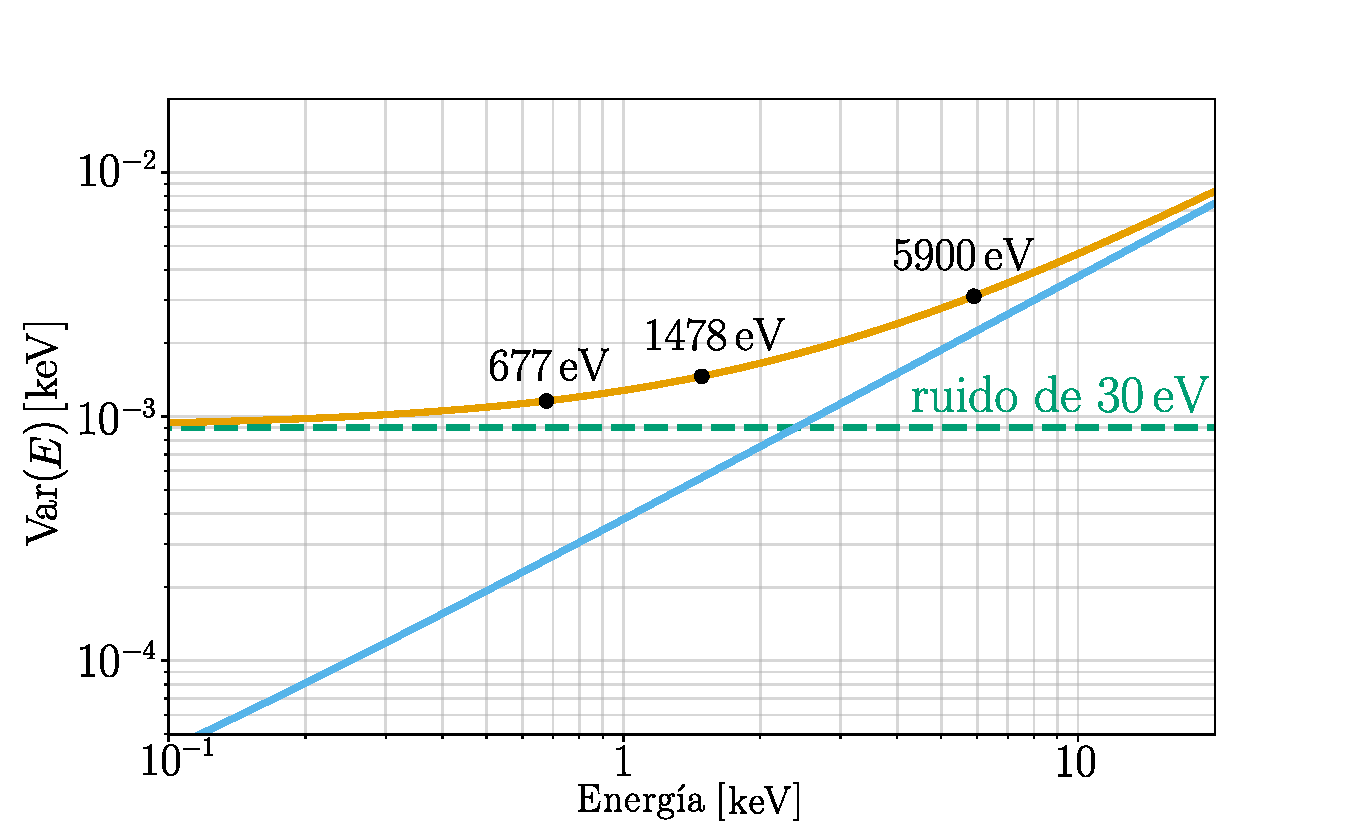
\includegraphics[scale=0.5]{Figs/fano_y_ruido.pdf}
    \caption{Valores que se obtendrían de medir el factor de Fano con un sensor CCD convencional (puntos negros), debido a la contribución del ruido de lectura constante de $30\,\si{eV}$ (línea punteada horizontal). La línea recta de trazo continuo representa un valor de factor de Fano constante de $F = 0.119$.}
    \label{fig:Fano_y_ruido}
\end{figure}

Los sensores \textit{Skipper}-CCD's, por otro lado, permiten disminuir el ruido de lectura a niveles subelectrónicos gracias a que son capaces de medir la carga en los píxeles de forma no destructiva. Esto permite tomar tantas mediciones de la carga como sean necesarias y estimar la carga real a partir de un promedio sobre el número de mediciones tomadas. 
Esta es la principal razón que motiva este trabajo, donde se realiza un estudio sistemático del factor de Fano a bajas energías, tanto a $1450\,\si{eV}$ (rayos X del Al) y $677\,\si{eV}$ (rayos X del flúor).

%%%%%%%%%%%%%%%%%%%%%%%%%%%%%%%%%%%%%%%%%%%%%%%%%%%%%%%%%%%%%%%%%%
%%%%%%%%%%%%%%%%%%%%%%%%%%%%%%%%%%%%%%%%%%%%%%%%%%%%%%%%%%%%%%%%%%
\section{Eficiencia de colección de carga}
\noindent La Eficiencia de Colección de Carga o CCE (\textit{Charge Collection Efficiency}, por sus siglas en inglés) se define como la fracción del total de carga producida durante un evento de ionización que es efectivamente medida. 
Para sensores del tipo \textit{fully depleted}-CCD\cite{osti_838066}, a los que se les aplican campos eléctricos relativamente altos, la CCE es aproximadamente del $100\,\%$, es decir, toda la carga producida por ionización en el volumen del sensor logra ser colectada y medida. 
Sin embargo, existen casos donde la eficiencia no alcanza el $100\,\%$ y esto es debido al fenómeno de Colección Parcial de Carga o PCC (\textit{Partial Charge Collection}, por sus siglas en inglés)\cite{PCC-CCE}. 
Este efecto se debe a que en los primeros micrones cercanos a la superficie por donde se irradia el detector (lado opuesto al que posea la superficie pixelada) existe una probabilidad no nula de que la carga generada por ionización sufra recombinación, es decir, que vuelva a enlazarse a un átomo. Este efecto produce una disminución en el número de cargas que finalmente son llevadas a la superficie del sensor. 
En el esquema de la Figura \ref{fig:PCC} se presenta una vista esquemática en corte lateral de las primeras centenas de nanómetros de un CCD, donde debido al ángulo $\theta$ de incidencia de los rayos $X$ de la fuente, estos fotones generan cargas por ionización en la región donde hay recombinación. Una fracción de las cargas generadas $q_{i}$ logran ser colectadas, dependiendo de la profundidad del sensor donde se produjo la interacción. También se muestra que si la interacción se da fuera de esta región, toda la carga generada por ionización es colectada, teniéndose $q_{i} = q_{f}$ y la eficiencia es máxima.
\begin{figure}%[H]
%Como reproducir este gráfico: correr el script NivelesOcupacionCarga.py ubicado en /Escritorio/Tesis2021/Figs/pys_para_plots y buscar la imagen en /home/igna/Escritorio/Tesis2021/Figs/
    \centering
        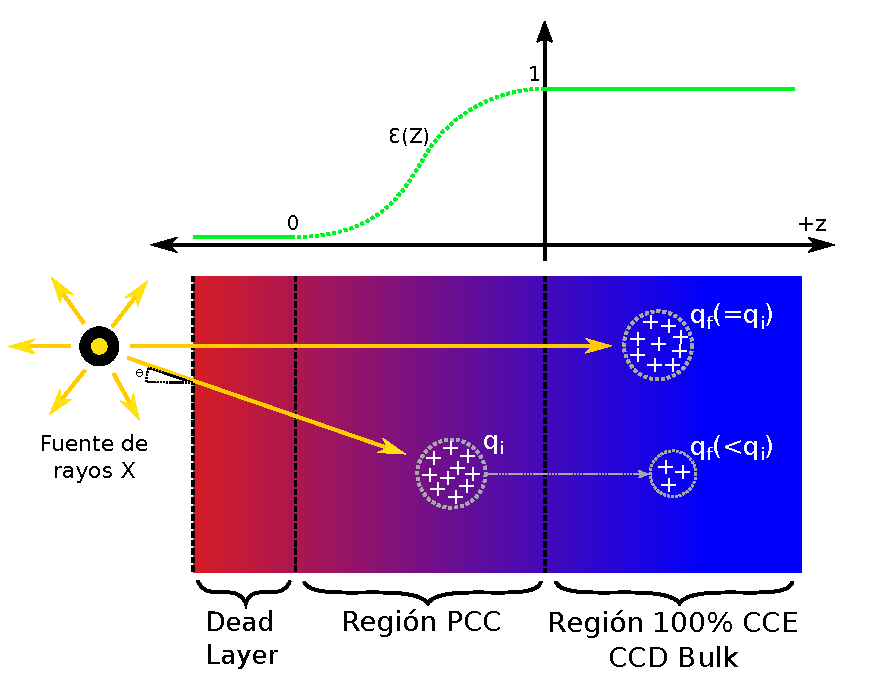
\includegraphics[scale=.8]{Figs/PCC.pdf}
    \caption{Esquema lateral de las primeras centenas de nanómetros de un CCD, con una fuente de rayos $X$\cite{PCC-CCE}. Los fotones penetran en el sensor produciendo una nube de cargas $q_{i}$, de las cuales solo una fracción logra ser colectada. Esta aumentan monótonamente dependiendo de la profundidad de penetración.}
    \label{fig:PCC}
\end{figure}
La colección parcial de carga es un problema propio de los sensores y de su fabricación. Sin embargo, existen tratamientos de la superficie posterior de estos sensores para reducir su impacto y que en general son aplicados en CCDs destinados a toma de imágenes astronómicas. 

El efecto que provoca la colección parcial de carga en las mediciones es el de agregar eventos con menor cantidad de carga de la que deberían, generando así colas a la izquierda de los picos de interés en los espectros y, por ende, agregando otro sesgo a la determinación de magnitudes dependientes del valor medio de los picos, como el factor de Fano.

%Por otro lado, la profundidad de la interacción depende del ángulo de incidencia y su distribución de probabilidad se puede escribir como
%\begin{equation*}
%    f_{Z}(z) = \frac{\cos{(\theta)}}{\lambda}e^{-z\frac{\cos{(\theta)}}{\lambda}}
%\end{equation*}
%donde $\lambda$ es la longitud de atenuación del fotón y depende de su longitud de onda. $\varepsilon(z)$ es la función \textit{eficiencia de colección de carga}
%\textcolor{red}{Reformulo lo anterior sin la dependencia con $\theta$}:

%%%%%%%%%%%%%%%%%%%%%%%%%%%%%%%%%%%%%%%%%%%%%%%%%%%%%%%%%%%%%%%%%%
%%%%%%%%%%%%%%%%%%%%%%%%%%%%%%%%%%%%%%%%%%%%%%%%%%%%%%%%%%%%%%%%%%

\section{Antecedentes \label{sec:Antecedentes}}
\noindent En trabajos previos se han estudiado las ventajas de la utilización de la tecnología \textit{Skipper} en los CCDs, para lograr medir con precisión subelectrónica en regímenes de energía donde los sensores CCD convencionales más precisos sólo podrían alcanzar resoluciones del orden de los $2$ electrones. Por primera vez fue usada para medir el factor de Fano y la energía de creación electrón-hueco en el silicio a una energía de $5.9\,\si{keV}$ a $123\,\si{K}$\cite{Rodrigues}.

Para lograr esto, se implementó un método de calibración absoluta de la relación entre el número de electrones en cada píxel y el valor de lectura en ADUs (\textit{Analog Digital Unit} o Unidades analógico-digitales). El procedimiento para la calibración consistió en la utilización de un LED que emitía fotones en $405\,\si{nm}$ de longitud de onda para poblar de carga los píxeles del sensor. Realizando un barrido en el tiempo de exposición del sensor a la luz del LED, se logró poblar a los píxeles del sensor con un amplio rango de cargas. La medición de carga se realizó tomando $300$ lecturas por cada píxel, que luego fueron promediadas logrando reducir el ruido de lectura en un factor $\sqrt{300}$. Como resultado, se obtuvieron distribuciones de carga gaussianas en los posibles niveles de ocupación de carga con una resolución tal que hizo posible distinguir perfectamente entre picos consecutivos, como se puede ver en la Figura \ref{fig:Calibracion}. De esta forma, mediante un ajuste gaussiano se pudo establecer el valor medio en ADUs para cada uno de estos picos, estableciendo como valor correspondiente de carga el número de orden del pico en cuestión. Así es que se obtuvo una relación uno a uno entre cantidad de carga por píxel y ADUs. Cabe destacar que para comenzar a numerar los picos, primero es necesario establecer el valor de $0$ carga o píxel vacío, lo cual no corresponde, a priori, a un valor nulo en ADUs. Para ello, las imágenes tomadas con \textit{Skipper} cuentan con una región denominada \textit{over-scan} que se utiliza para calcular la línea de base y poder sustraerla luego al valor en ADU medido para cada píxel, logrando así que la media de los píxeles vacíos quede en cero ADUs.
\begin{figure}[H]
%Como reproducir este gráfico: correr el script NivelesOcupacionCarga.py ubicado en /Escritorio/Tesis2021/Figs/pys_para_plots y buscar la imagen en /home/igna/Escritorio/Tesis2021/Figs/
    \centering
        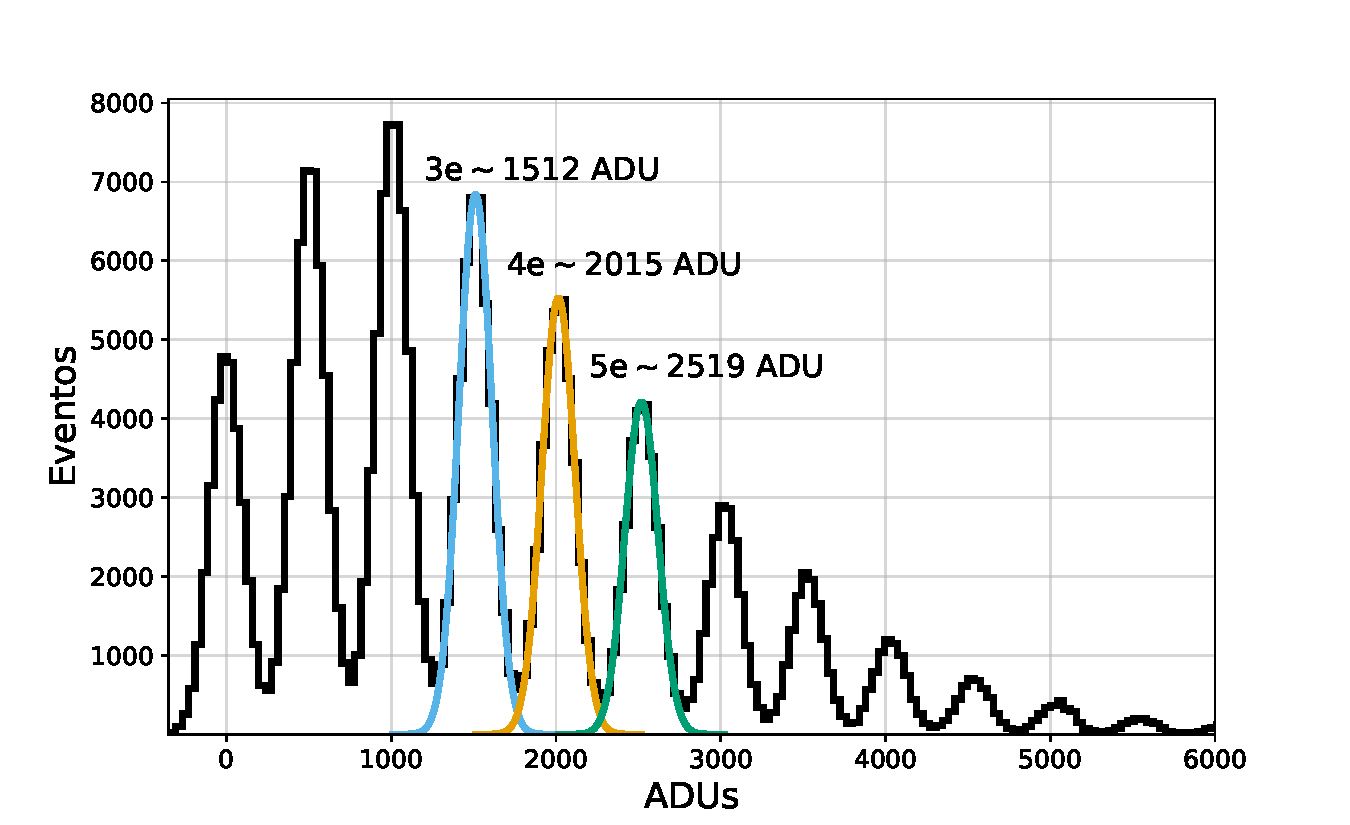
\includegraphics[scale=0.5]{Figs/ajuste_gaussiano_calibracion.pdf}
    \caption{Histograma de los datos obtenidos al iluminar el CCD con LED, correspondiente a una región con poca ocupación, donde los picos de los niveles de carga y su ajuste se distinguen a la perfección.}
    \label{fig:Calibracion}
\end{figure}
Las mediciones del factor de Fano y la energía de creación electrón-hueco se realizaron utilizando rayos $X$ de $5.9\,\si{\mbox{keV}}$ emitidos por una fuente de $\Fe{55}$. Más precisamente, rayos $X_{K}$, cuyas energías son las de la Tabla \ref{tab:EnergiasXk}.
\begin{table}[h]
\centering
\begin{tabular}{@{}ccc@{}}
\toprule
$X_{K}$         &   Energía [keV]   &   Intensidad relativa \\ \hline \hline
$\alpha_{2}$    &   $5887.6$        &   $8.5 (4)$           \\
$\alpha_{1}$    &   $5898.8$        &   $16.9 (8)$          \\
$\beta_{3}$     &   $6490.4$        &   $4.1 (11)$          \\ \bottomrule
\end{tabular}
\caption{Energías e intensidades relativas de los fotones X emitidos tras el decaimiento de $\Fe{55}$}
\label{tab:EnergiasXk}
\end{table}
Sobre los histogramas de los espectros obtenidos al irradiar el CCD con estos rayos $X$, se realizó un ajuste de los picos del espectro para obtener los parámetros $\mu$ y $\sigma$ de cada uno. 
Para esto, se utilizó la verosimilitud de la ecuación \eqref{ec:verosimilitud}, que surge de convolucionar dos distribuciones exponenciales y una distribución gaussiana
{\small
\begin{align}
    \Lagr(e|\mu_{1},
            \mu_{2},
            \sigma_{1},
            \lambda_{1},
            \lambda_{2},
            \eta_{1} = \eta_{2},
            \eta_{3})
    = &
    \sum\limits_{j=1}^{3} I_{j}
    \left\{
        \eta_{j}\frac{\lambda_{1}}{2}
        \exp
            \left[
                (e-\mu_{j})\lambda_{1} + \frac{\sigma_{j}^{2}\lambda_{1}^{2}}{2}
            \right]
        \mbox{Erfc}
        \left[
            \frac{1}{\sqrt{2}}
            \left(
                \frac{e - \mu_{j}}{\sigma_{j}}
                +\sigma_{j}\lambda_{1}
            \right)
        \right] \right. \nonumber
        \\
        + &
        \left.
        (1-\eta_{j})\frac{\lambda_{2}}{2}
        \exp
            \left[
                 (e - \mu_{j})\lambda_{2}
                 + \frac{\sigma_{j}^{2}\lambda_{2}^{2}}{2}
            \right]
        \mbox{Erfc}
        \left[
            \frac{1}{\sqrt{2}}
            \left(
                \frac{e - \mu_{j}}{\sigma_{j}}
                +\sigma_{j}\lambda_{2}
            \right)
        \right]
    \right\}
        \label{ec:verosimilitud}
\end{align}
}%
donde $\mu_{j}$, $\sigma_{j}$ y $I_{j}$ representan el valor medio de carga, la desviación estándar del valor medio de carga y la intensidad relativa del pico $j$-ésimo con energía $E_{j}$, respectivamente y $j = \{\alpha_{1}, \alpha_{2}, \beta_{3}\}$. Además, $\lambda_{1}$ y $\lambda_{2}$ son parámetros de la distribuciones exponenciales y $\eta_{j}$ es el peso relativo entre ellas. Se utilizaron dos exponenciales y una gaussiana para modelar los picos con la intención de describir las colas que había a bajas energías, tomando la descripción que suele hacerse para picos en espectrometría $\alpha$\cite{Bortels}. Sin embargo, se sabe que en este último caso las colas son debidas al fenómeno de auto-absorción, el cual no está presente en los experimentos anteriormente mencionados. Puede decirse entonces que se trató de un modelo fenomenológico, es decir, no basado en primeros principios.
\begin{table}[h]
\centering
\begin{tabular*}{\textwidth}{c @{\extracolsep{\fill}} ccccccccc}%{@{}ccccccccc@{}}
\toprule
$X_{K}$ &
  $\mu\ [e^{-}]$ &
  $\Delta \mu\ [e^{-}]$ &
  $\sigma\ [e^{-}]$ &
  $\Delta \sigma\ [e^{-}]$ &
  $F$ &
  $\Delta F$ &
  $\varepsilon_{\eh}\ [\mbox{eV}/e^{-}]$ &
  $\Delta \varepsilon_{\eh} \ [\mbox{eV}/e^{-}]$ \\ \hline\hline
$\alpha_{2}$ &
  $1570.50$ &
  $0.18$ &
  $13.68$ &
  $0.12$ &
  \multirow{3}{*}{$0.119$} &
  \multirow{3}{*}{$0.002$} &
  \multirow{2}{*}{$3.749$} &
  \multirow{2}{*}{$0.001$} \\
$\alpha_{1}$ & $1573.48$ & $0.18$ & $13.69$ & $0.12$ &  &  &         &         \\
$\beta_{3}$  & $1730.50$ & $0.55$ & $14.36$ & $0.13$ &  &  & $3.751$ & $0.002$ \\ \bottomrule
\end{tabular*}
\caption{Parámetros obtenidos de los ajustes para las mediciones del $\Fe{55}$. El factor de Fano se tomó el mismo para los tres picos y la energía de creación electrón hueco se fijó para que sea la misma en los picos $\alpha$.}
\label{tab:ParametrosAjusteNoBineado}
\end{table}

Así es que los valores condensados en la Tabla \ref{tab:ParametrosAjusteNoBineado} constituyen los primeros resultados obtenidos de la utilización de la tecnología \textit{Skipper}-CCD para el cálculo del factor de Fano y de la energía de creación electrón-hueco para una temperatura de $123\,\si{K}$. Los mismos se encuentran en excelente acuerdo con la bibliografía preexistente~\cite{Ryan, Alig, Kotov} y presentan la mejor incerteza alcanzada a la fecha.

En esa oportunidad se llevaron a cabo además las primeras mediciones tendientes a determinar el factor de Fano y la energía de creación electrón-hueco para energías por debajo de los de $2\,\si{keV}$~\cite{TesisKevin}, más específicamente, para energías de $677\,\si{eV}$ y $1486\,\si{eV}$, que corresponden a los rayos $X$ de fluorescencia del flúor y del aluminio respectivamente. 
En la Tabla \ref{tab:EnergiasFluorescenciaFAl} pueden verse las energías e intensidades relativas para los rayos $X$ de estos elementos. 
Esto se logró a partir de mediciones realizadas con una fuente de $\Am{241}$ que emite partículas $\alpha$ con una energía de $\sim 5.6\,\si{MeV}$. 
A estas partículas se las hizo impactar contra una cinta de teflón (que contiene flúor) y una barra de aluminio que por fluorescencia emitían rayos $X$ con las energías antes mencionadas. 
\begin{table}[h]
\centering
\begin{tabular}{@{}cccc@{}}
\toprule
Elemento    &   $X_{K}$         &   Energía [eV]    &   Intensidad relativa \\ \hline \hline
F           &   $\alpha_{1,2}$  &   $676.8$         &   $148$               \\
Al          &   $\alpha_{2}$    &   $1486.3$        &   $50$                \\
Al          &   $\alpha_{1}$    &   $1486.7$        &   $100$               \\
Al          &   $\beta_{1}$     &   $1557.4$        &   $1$                 \\ \bottomrule
\end{tabular}
\caption{Energías e intensidades de las líneas de emisión de rayos $X$ para el flúor y el aluminio en el rango de energías por debajo de los $2\,\si{keV}$.}
\label{tab:EnergiasFluorescenciaFAl}
\end{table}

Uno de los desafíos que surgieron en este otro trabajo fue obtener una buena estadística, debido a que solo una fracción muy pequeña de los átomos que son impactados por las partículas $\alpha$ se desexcitan emitiendo fotones $X$ en las energías de interés. La emisión de rayos $X$ tras la captura electrónica del núcleo del $\Fe{55}$, en cambio, ocurre siempre y por lo tanto es proporcional a la actividad de la fuente. Por esta razón, dada una misma actividad de la fuente de $\Fe{55}$ y la tasa de emisión de partículas $\alpha$, la obtención de rayos $X$ es mucho más probable en el primer caso, haciendo la colección de eventos más rápida.

Con los datos de estas mediciones se reconstruyeron los espectros para ambos picos y se les realizó un ajuste muy similar al de los experimentos con $\Fe{55}$, utilizando la verosimilitud descripta por la expresión \eqref{ec:verosimilitudF-Al}
\begin{align}
    \Lagr(e|\mu,
            \sigma,
            \lambda_{1},
            \lambda_{2},
            \eta)
    = &
    \eta
    \left\{
        \frac{\lambda_{1}}{2}
        \exp\left[
                (e-\mu)\lambda_{1} + \frac{\sigma^{2}\lambda_{1}^{2}}{2}
            \right]
        \mbox{Erfc}
        \left[
            \frac{1}{\sqrt{2}}
            \left(
                \frac{e - \mu}{\sigma}
                +\sigma\lambda_{1}
            \right)
        \right] \right\} \nonumber
        \\
        + &
        (1-\eta)
        \left\{
        \frac{\lambda_{2}}{2}
        \exp
            \left[
                 (e - \mu)\lambda_{2}
                 + \frac{\sigma^{2}\lambda_{2}^{2}}{2}
            \right]
        \mbox{Erfc}
        \left[
            \frac{1}{\sqrt{2}}
            \left(
                \frac{e - \mu}{\sigma}
                +\sigma\lambda_{2}
            \right)
        \right]
    \right\}
        \label{ec:verosimilitudF-Al}
\end{align}

Los resultados obtenidos en este trabajo se encuentran en la Tabla \ref{tab:ParametrosAjusteNoBineadoF-Al}.
\begin{table}[h]
\centering
\begin{tabular*}{\textwidth}{c @{\extracolsep{\fill}} ccccccccc}%{@{}ccccccccc@{}}
\toprule
Elemento&
  $\mu\ [e^{-}]$ &
  $\Delta \mu\ [e^{-}]$ &
  $\sigma\ [e^{-}]$ &
  $\Delta \sigma\ [e^{-}]$ &
  $F$ &
  $\Delta F$ &
  $\varepsilon_{\eh}\ [\mbox{eV}/e^{-}]$ &
  $\Delta \varepsilon_{\eh} \ [\mbox{eV}/e^{-}]$ \\ \hline\hline
  F &   $182.0$ &   $0.8$  &   $7.0$   &   $0.7$   &   $0.27$  &   $0.05$  &   $3.72$ &   $0.02$\\
  Al&   $404.4$ &   $0.4$  &   $8.3$   &   $0.3$   &   $0.17$  &   $0.01$  &   $3.679$ &   $0.004$\\ \bottomrule
\end{tabular*}
\caption{Resultados preliminares obtenidos en un trabajo previo para el factor de Fano y la energía de creación electrón-hueco para las energías de los rayos $X$ de fluorescencia del flúor y el aluminio.}
\label{tab:ParametrosAjusteNoBineadoF-Al}
\end{table}

Sin embargo, estos últimos fueron resultados preliminares que podían mejorarse tanto aumentando la estadística, como realizando un análisis de los datos más sofisticado. Sobre este último punto, vale decir que el modelo de ajuste utilizado antes de esta tesis no incluye los efectos de la colección parcial de carga. Además, en el análisis de las imágenes, no se realizó ninguna corrección por el sesgo que podría significar la adición de carga originada por fuentes de fondo descriptas en la próxima sección.

Es a partir de aquí donde este trabajo continua con el estudio del factor de Fano, la energía de creación electrón hueco y la colección parcial de carga, a partir de mediciones de rayos X con energías por debajo de los $2\,\si{keV}$.

%%%%%%%%%%%%%%%%%%%%%%%%%%%%%%%%%%%%%%%%%%%%%%%%%%%%%%%%%%%%%%%%%%
%%%%%%%%%%%%%%%%%%%%%%%%%%%%%%%%%%%%%%%%%%%%%%%%%%%%%%%%%%%%%%%%%%
\section{Motivación del análisis de imágenes}
\noindent El fondo presente en las imágenes tiene diferentes orígenes, uno de ellos es la carga producida por fluctuaciones térmicas en la red cristalina del silicio del sensor (corrientes oscuras). Otra contribución es la de eventos de dispersión Compton, producidos por la interacción de los fotones con los materiales que rodean al sensor y también en la red cristalina del mismo. Podemos incluir además, aquellos fotones infrarrojos emitidos desde los materiales que rodean al detector cuando estos son excitados por radiación circundante o bien por radiación de cuerpo negro. También se encuentran los eventos de carga producida por radiación muy penetrante provenientes del exterior, como por ejemplo, muones.

\textcolor{red}{Nunca se dijo que es un cluster, ni porque aparecen. Hay que contarlo y mencionar la difusion como parte del proceso.}
Parte del análisis consistió en estudiar el efecto que produce el fondo de las imágenes sobre los eventos de interés: la aglomeración de píxeles con un único electrón alrededor de los clusters, y la carga extra añadida sobre ellos. 
En muchos casos resulta que los píxeles con fondo se aglutinan a los clusters, aumentando su tamaño y su carga, o incluso también haciendo de puente entre dos clusters vecinos. Estos son dos efectos indeseados, primero, porque sesgan la cantidad de carga real en un evento de interés y segundo, porque los programas de reconocimiento de eventos podrían ignorarlos al no cumplir con los cortes de calidad impuestos\footnote{Ver sección \ref{sec:ProcesadoDatos}}, tanto por forma como por cantidad de carga, produciendo así una disminución en la estadística.

En este contexto, se propone utilizar un umbral de detección que ignore píxeles con un sólo electrón, de forma de evitar el aglutinamiento de píxeles con fondo a los clusters de interés y así aumentar la estadística en el conteo de eventos. Pero también es necesario lograr caracterizar el fondo responsable de este efecto para corregir el sesgo introducido por el nuevo umbral de detección, el cual también eliminará píxeles con una carga genuina.
%En este contexto, se propone utilizar un umbral de detección que ignore píxeles con un sólo electrón, de forma de evitar un píxel con una carga originada en eventos de fondo se adicione a un cluster de interés, haciendo que este entre en contacto con un tercero, dando lugar al aglutinamiento de clusters de interés. La carga neta del nuevo cluster haría que el mismo deje de encontrarse entre los de interés. Por lo tanto, evitar este efecto debe redundar en un aumento de la estadística.
%Pero también es necesario lograr caracterizar el fondo responsable de este efecto para corregir el sesgo introducido por el nuevo umbral de detección que elimina eventos de un electrón, el cual, también eliminará píxeles con una carga genuina.
%########################################################################
% NACHO NOTE: perdón pero esto lo revertí porque no me gustaba nada el primer párrafo. Da información que se da en la sección 4.2 (4to párrafo aprox), aca mi idea era superficialmente tirar la motivación
%########################################################################
Es por eso que en este trabajo se propuso un análisis de las imágenes que pueda corregir el sesgo introducido luego de recuperar la mayor estadística posible separando eventos unidos por un electrón de fondo. 
Esto es, el desarrollo de un método para estimar en valores medios cuántos electrones genuinos son removidos y cuántos electrones espurios hay en los eventos, para mejorar así las incertezas en la determinación del factor de Fano y la energía de creación electrón-hueco a bajas energías.

Motiva también este trabajo el desarrollo y aplicación de un modelo que permita dar cuenta del efecto de colección parcial de carga y así obtener una forma analítica para la distribución de carga producida por los fotones de interés.

%%%%%%%%%%%%%%%%%%%%%%%%%%%%%%%%%%%%%%%%%%%%%%%%%%%%%%%%%%%%%%%%%%
%%%%%%%%%%%%%%%%%%%%%%%%%%%%%%%%%%%%%%%%%%%%%%%%%%%%%%%%%%%%%%%%%%
\section{Organización de la tesis}
\noindent En el presente capítulo se ha dado una breve introducción a los tres aspectos principales de estudio de este trabajo: el factor de Fano, la energía de creación electrón hueco y la colección parcial de carga. Además se han presentado resultados que conforman los antecedentes para la motivación de esta tesis.

En el capítulo \ref{chap:simulaciones} se presenta un modelo físico simple de la interacción entre fotones incidentes y la red del sensor, que luego es estudiado a partir de simulaciones Monte Carlo.

En el capítulo \ref{chap:ConfiguracionExperimental} se desarrolla una descripción esquemática del dispositivo de medición utilizado y los regímenes de trabajo necesarios para realizar las mediciones. También se da una breve descripción del sensor y de los materiales que lo componen, como así también de la fuente radioactiva utilizada. Por último, se describe el proceso de medición.

En el capítulo \ref{chap:Analisis} se describe cómo son procesados los datos y qué programas son utilizados además de las pruebas realizadas con distintos umbrales. También se muestran diferentes análisis de caracterización del sensor. Es en este capítulo que se describen los diferentes enfoques utilizados en la estimación del fondo y de la cantidad de eventos eliminados por el umbral y el método aplicado para realizar las correcciones sobre la carga.

En el capítulo \ref{chap:ModeloPCC} se introduce un modelo que describe la distribución de carga considerando no solo el factor de Fano sino además el de colección parcial de carga. 

Por último, en el capítulo \ref{chap:Resultados} se presentan los resultados obtenidos a partir de ajustes no bineados, utilizando el modelo descripto en el capítulo \ref{chap:ModeloPCC} y las perspectivas a futuro.


%%%%%%%%%%%%%%%%%%%%%%%%%%%%%%%%%%%%%%%%%%%%%%%%%%%%%%%%%%%%%%%%%%
%%%%%%%%%%%%%%%%%%%%%%%%%%%%%%%%%%%%%%%%%%%%%%%%%%%%%%%%%%%%%%%%%%
%%%%%%%%%%%%%%%%%%%%%%%%%%%%%%%%%%%%%%%%%%%%%%%%%%%%%%%%%%%%%%%%%%
    
    \chapter{Ionización del medio y simulaciones Monte Carlo}
%%%%%%%%%%%%%%%%%%%%%%%%%%%%%%%%%%%%%%%%%%%%%%%%%%%%%%%%%%%%%%%%%%
%%%%%%%%%%%%%%%%%%%%%%%%%%%%%%%%%%%%%%%%%%%%%%%%%%%%%%%%%%%%%%%%%%
\section{Modelado del fenómeno físico}
\noindent Uno de los interrogantes que se propuso responder en este trabajo es por qué el factor de Fano del sensor no vale $1$, independientemente de la energía depositada, dado que para todo proceso Poissoniano, la relación entre la varianza y la esperanza vale
\begin{equation*}
    F = \frac{\sigma^{2}}{\mu} = 1
\end{equation*} 
El factor de Fano del sensor se calcula hallando el valor medio $\mu$ y la varianza $\sigma^{2}$ de la distribución de carga correspondiente a los eventos de interés, como por ejemplo, los picos de los espectros generados por los rayos $X$ del Flúor o el Aluminio. \textcolor{red}{Se sabe que el número de fotones emitidos por una fuente radioactiva sigue una distribución Poissoniana, de la misma manera la cantidad de carga ionizada en el sensor, producto de la interacción con estos fotones, también es Poissoniana.} Sin embargo, experimentalmente se observa que cuando toda la energía de la partícula incidente es depositada en el material, el factor de Fano resulta casi un orden de magnitud menor\cite{TesisKevin}. Una de las posibles razones por las que esto sucede es que la energía de los fotones incidentes no solo es disipada en forma de ionización de carga, si no también en excitación de fonones de la red cristalina del material.\\
\indent Cuando un fotón de alta energía cinética impacta contra el sensor, este produce una dispersión por ionización y emisión de fonones de la red cristalina del Silicio, produciendo así una cascada de pares electrón-hueco. El número de pares producidos puede ser luego medido y el valor de la energía de creación electrón-hueco promediado a partir de este.\\
\indent Este fenómeno es estudiando en los trabajos de R.C. Alig et al.\cite{Alig}, mediante simulaciones de Monte Carlo y luego por K. Ramanathan \cite{Ramanathan}, compilando resultados y propuestas de diferentes trabajos. En el primero se propone un modelo en el que la partícula incidente interactúa con el material, generando pares electrón-hueco por ionización en forma de cascada y, eventualmente, perdiendo energía por emisión de fonones. La forma en el que la partícula incidente va perdiendo energía depende fuertemente de la energía que tiene al momento de generar un par electrón-hueco. Esta dependencia está modelada en el segundo trabajo y lo llaman \textit{modelo simplificado}, donde proponen que la energía $E$ que se transfiere a para generar pares electrón-hueco se reparte según una distribución Beta, de la forma
\begin{equation*}
    p(x|\alpha) = \frac{2}{B(\alpha)} x^{\alpha - 1}(1-x)^{\alpha - 1}
\end{equation*}
donde $x = \frac{E}{E_{r} - E_{g}}$ es la variable aleatoria, con $E_{r}$ la energía inicial de la partícula en cada ionización, $E_{g}$ es la energía del gap del Silicio y $E$ la fracción de energía que va a parar a un nuevo par electrón hueco. Utilizando esta distribución para generar realizaciones de la variable aleatoria $x$, se puede despejar el valor de $E$ que es la energía transferida para generar pares electrón-hueco según este modelo. Por otro lado, $B(\alpha)$ es la función Beta con un único parámetro $\alpha$, y viene dada por
\begin{equation*}
    B(\alpha, \beta) 
    = \frac{\Gamma(\alpha)\Gamma(\beta)}{\Gamma(\alpha) + \Gamma(\beta)}
    \longrightarrow
    B(\alpha)
    = \frac{\Gamma^{2}(\alpha)}{2\Gamma(\alpha)}
\end{equation*}
donde $\alpha$ depende de la energía $E_{r}$ y es el parámetro que determina el régimen de distribución de la energía, o en otras palabras, la forma de la distribución.\\
\indent La razón de la utilización de la distribución Beta para modelar cómo se reparte la energía en la generación de pares electrón-hueco por ionización se debe a que esta se adapta muy bien a los tres tipos de regímenes de energía en los que se puede encontrar la partícula incidente, según los trabajos mencionados anteriormente:
\begin{itemize}
    \item \textbf{A bajas energías de la partícula incidente}, se tienen distribuciones muy picudas en los extremos posibles: $E = 0$ y $E = E_{R}+E_{g}$,
    \item \textbf{A energías mucho mayores que la energía del gap}, $E_{R} >> E_{g}$: Se tiene una distribución aproximadamente uniforme,
    \item \textbf{A energías entre $3.4\,\si{eV}$ - $4.2\,\si{eV}$} se tiene una distribución de energía muy picuda en el medio de $x = E/(E_{R} - E_{g})$.
\end{itemize}
Para energías bajas, el parámetro $\alpha$ tiende a cero y se tiene una distribución con máximos en los extremos del intervalo. Para energías entre $3.4\,\si{eV}$ y $4.2\,\si{eV}$ se tiene una distribución con un máximo en el medio del intervalo y el parámetro $\alpha$ puede tender a infinito. Por último, para energías mucho mayores a la energía del gap, el parámetro $\alpha = 1$ y la distribución es uniforme. Estos casos se resumen el gráfico de la figura \ref{fig:BetaDist}.
\begin{figure}%[H]
% Este gráfico se hace con el script que está acá: /home/igna/Escritorio/Tesis2021/Figs/Figuras_Apendice_Simulaciones/pys_para_plots DistBetaFig.py
    \centering
    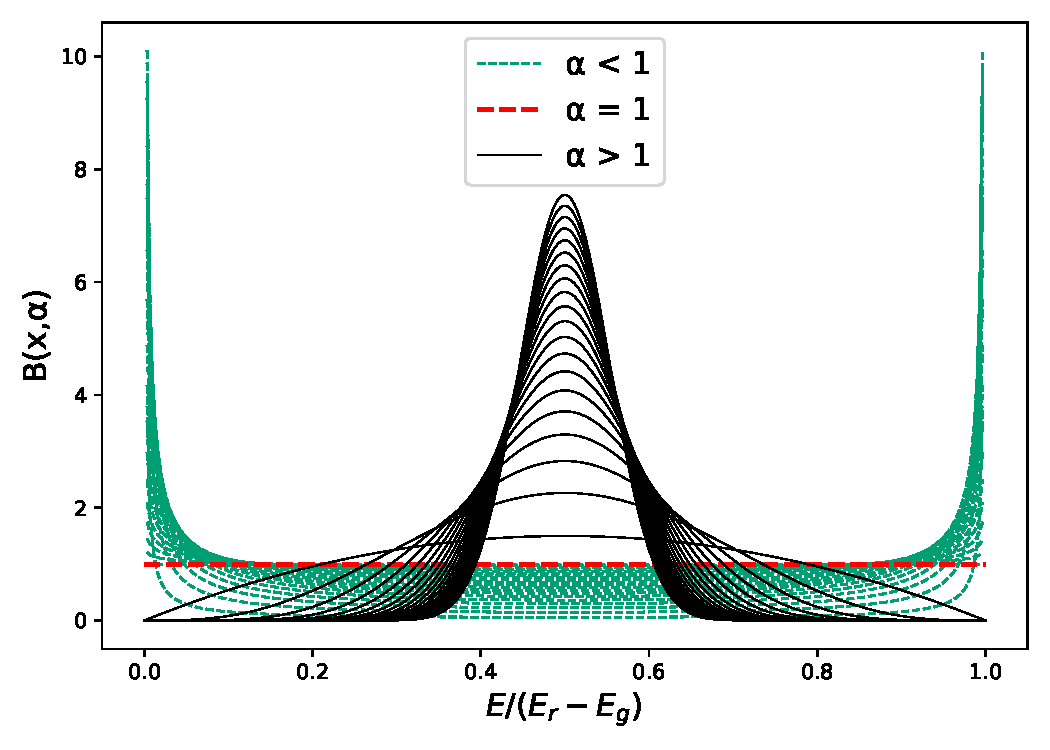
\includegraphics[scale=.7]{Figs/BetaDistFig.pdf}
    \caption{\footnotesize{Distribución Beta para diferentes valores del parámetro $\alpha$}}
    \label{fig:BetaDist}
\end{figure}
El mecanismo de cascada por el cual se producen las ionizaciones consiste en que para una dada energía inicial $E_{R}$, una fracción de esa energía se utiliza para generar un par electrón-hueco y la energía restante vuelve a fraccionarse para generar otros pares electrón-hueco. Estos pares generados, a su vez, utilizan fracciones de esa energía que les fue entregada para generar otros pares, en un proceso que se repite hasta que la energía disponible para repartir en cada rama de la cascada es menor a la energía del gap del Silicio y ya no es suficiente para generar más pares. Durante todo este proceso existe una probabilidad no nula de que parte de la energía se pierda por emisión fonones en la red.\\
\indent Se define una probabilidad $P_{eh}$ para la cual se produce ionización y una probabilidad $1 - P_{eh}$ para la cual se produce emisión de fonones. Esta probabilidad depende de la energía inicial, al igual que el parámetro $\alpha$ de la distribución Beta, y viene dada por
\begin{equation}
    P_{eh}(E_{R}) = 
    \left[
        1 + \frac{\Gamma_{ph}(E_{R})}{\Gamma_{eh}(E_{R})}
    \right]^{-1}
        \label{ec:ProbabilidadIonizacion}
\end{equation}
donde 
\begin{equation*}
    \frac{\Gamma_{ph}(E_{R})}{\Gamma_{eh}(E_{R})}
    = A\frac{105}{2\pi}\frac{(E_{R} - \hbar \omega_{0})^{1/2}}{(E_{R} - E_{g})^{7/2}}
\end{equation*}
con $A = 5.2\,eV^{3}$, que es una constante fenomenológica que contiene información microscópica del sistema y que además puede ajustarse para reproducir valores medidos experimentalmente. Por otro lado, $\Gamma_{ph}$ y $\Gamma_{eh}$ son las tasas de producción de fonones y pares electrón-hueco, respectivamente.\\
\indent Partiendo de estas ideas, se buscó simular este mecanismo de ionización a partir de simulaciones Monte Carlo.
%%%%%%%%%%%%%%%%%%%%%%%%%%%%%%%%%%%%%%%%%%%%%%%%%%%%%%%%%%%%%%%%%%
%%%%%%%%%%%%%%%%%%%%%%%%%%%%%%%%%%%%%%%%%%%%%%%%%%%%%%%%%%%%%%%%%%
\section{Simulaciones básicas}
\noindent La aproximación a orden cero del mecanismo de ionización puede pensarse como una serie de experimentos de Bernoulli de éxito-fracaso, con una dada probabilidad de éxito $p$, que es la probabilidad de ionizar una carga y perder una cantidad de energía equivalente a la energía de creación electrón-hueco del Silicio, sin tener en cuenta explícitamente la disipación de energía por excitación de fonones.\\
\indent Dada una energía inicial y número fijo de experimentos de Bernoulli $N$ (que viene a modelar en cierta forma el ancho del material o la cantidad de veces que la partícula incidente puede interactuar con la red), puede suceder que la energía inicial se agote completamente o no. El valor final de la energía depende muy fuertemente del valor de $N$: Para una cantidad de experimentos $N$ muy grande, la probabilidad de que la energía se agote completamente es muy alta, mientras que para $N$ muy pequeño la probabilidad es mucho menor, pudiendo suceder que la energía no sea cero al final del experimento. No es sorprendente que con este modelo se recupera un factor de Fano que tiende a $1$, en el caso en el que el valor de $N$ es grande pero no suficiente para agotar la energía de la partícula incidente, debido a que la distribución binomial que surge de la realización de experimentos consecutivos de Bernoulli tiende a una distribución de Poisson si $p$ es pequeño. Esto puede verse en la figura \ref{fig:SimulacionOrden0Fano1}, donde claramente puede verse que una distribución Poissoniana ajusta muy bien al histograma. Esta corresponde a una simulación que parte de una energía inicial de $677\,\si{eV}$ con un $N = 5000$, que es la cantidad de veces que se repite el experimento de Bernoulli de ionizar o no con probabilidad $p=0.01$ y el factor de Fano resultó $F = 0.991$. A su vez, este experimento se repitió $20000$ veces para tener una buena cantidad de estadística para formar el histograma.\\
\begin{figure}%[H]
%Para hacer este gráfico hay que correr el script que está en esta carpeta /home/igna/Escritorio/Tesis2021/Figs/Figuras_Apendice_Simulaciones/pys_para_plots y se llama Orden0_simu_SI_atraviesa.py con los datos de esta carpeta /home/igna/Escritorio/Tesis2021/Figs/Figuras_Apendice_Simulaciones/txts_para_plots y se llama orden0_simu_SI_atraviesa.txt
    \centering
    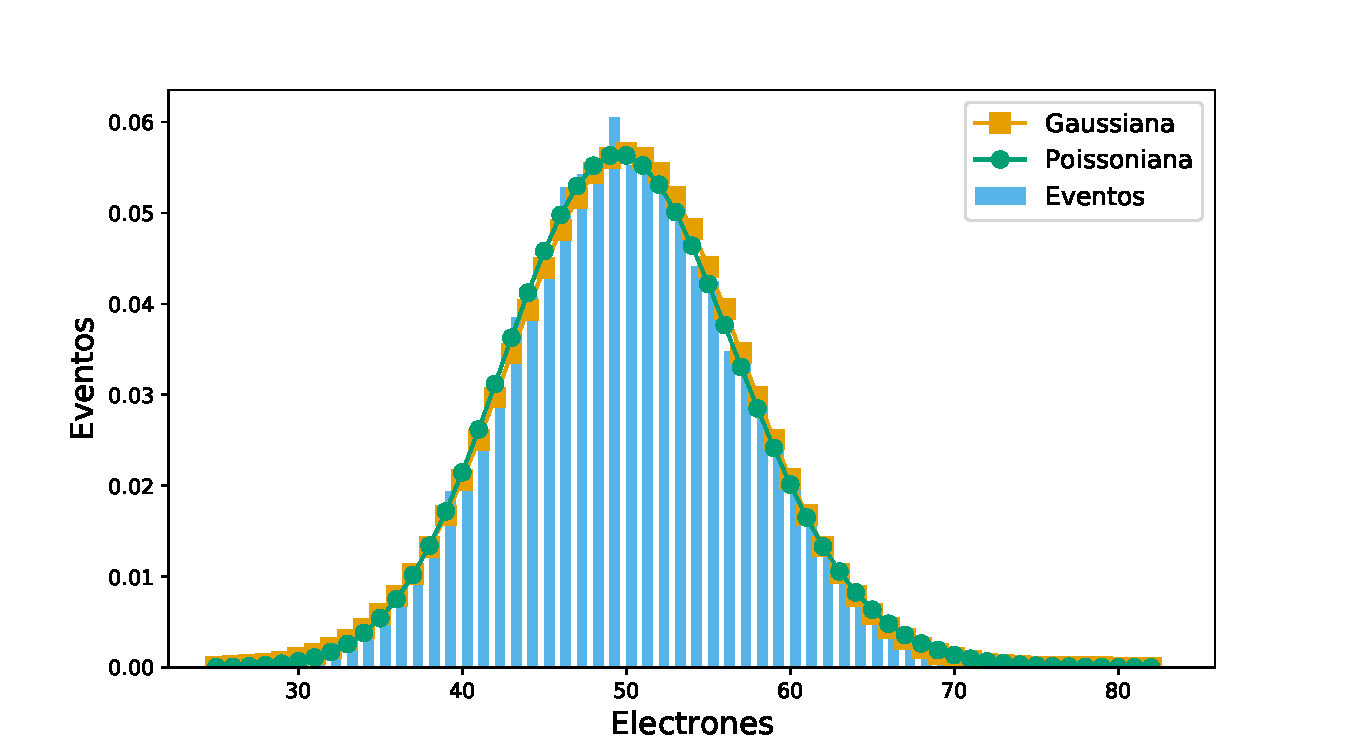
\includegraphics[scale=0.35]{Figs/Orden0_fano1.pdf}
    \caption{\footnotesize{Como reproducir esta imagen: Directorio (base) igna@Igna:~/Escritorio/Tesis2021/simulacion electrones\$ y correr ./SimuC2PyandPlot.py con parámetros: trials = 20000, distancia = 5000, atraviesa = 0 y branch git Master}}
    \label{fig:SimulacionOrden0Fano1}
\end{figure}
\indent Por el contrario, para el caso en que $N$ es tal que la gran mayoría de las veces la energía se agota completamente, el factor de Fano se vuelve menor a $1$, como puede verse en la figura \ref{fig:SimulacionOrden0Fano0}. En este caso, nuevamente se parte de una energía inicial de $677\,\si{eV}$ pero esta vez con un $N = 30000$, cantidad suficiente para agotar completamente la energía y $p=0.01$ nuevamente. Se repitió $20000$ veces el experimento para obtener una buena cantidad de estadística para formar el histograma. En este caso el factor de Fano fue de $F = 0.297$.\\
\begin{figure}%[h]
%Para hacer este gráfico hay que correr el script que está en esta carpeta /home/igna/Escritorio/Tesis2021/Figs/Figuras_Apendice_Simulaciones/pys_para_plots y se llama Orden0_simu_NO_atraviesa.py con los datos de esta carpeta /home/igna/Escritorio/Tesis2021/Figs/Figuras_Apendice_Simulaciones/txts_para_plots y se llama orden0_simu_NO_atraviesa.txt
    \centering
    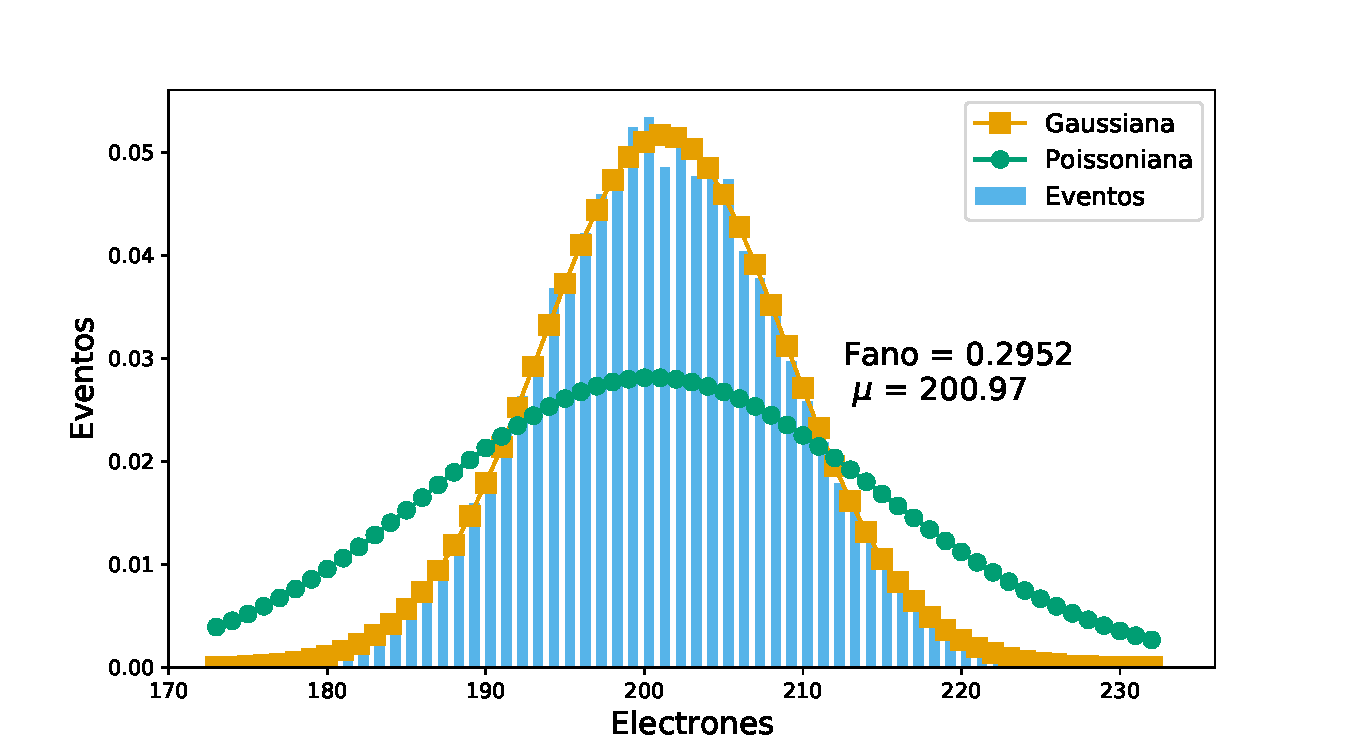
\includegraphics[scale=0.35]{Figs/Orden0_fano0.pdf}
    \caption{\footnotesize{Como reproducir esta imagen: Directorio (base) igna@Igna:~/Escritorio/Tesis2021/simulacion electrones\$ y correr ./SimuC2PyandPlot.py con parámetros: trials = 20000, distancia = 30000, atraviesa = 0 y branch git Master}}
    \label{fig:SimulacionOrden0Fano0}
\end{figure}
\indent Si bien este modelo de juguete es una simplificación del proceso de dispersión real, los resultados de este están en concordancia con la hipótesis de que el factor de Fano es menor a $1$ debido a que la partícula incidente deposita toda su energía en el material.\\
%%%%%%%%%%%%%%%%%%%%%%%%%%%%%%%%%%%%%%%%%%%%%%%%%%%%%%%%%%%%%%%%%%
%%%%%%%%%%%%%%%%%%%%%%%%%%%%%%%%%%%%%%%%%%%%%%%%%%%%%%%%%%%%%%%%%%
\section{Simulación de ionización en cascada}
\noindent Utilizando ideas tomadas de los trabajos anteriormente citados, se modificaron las simulaciones Monte Carlo para intentar reproducir el mecanismo de creación de pares electrón-hueco por ionización en cascada. Para este caso se tuvo en cuenta la posibilidad de disipación de energía por emisión de fonones, a una energía fija de $\hbar\omega_{0} = 0.063\,eV$.\\
\indent El resultado de la simulación es simplemente el número de pares 
ionizados a partir de la energía inicial $E_{R}$. De esta puede verse la distribución de la cantidad de pares generados y además calcular tanto su varianza como su esperanza, para así obtener el factor de Fano.\\
\indent Otro factor a tener en cuenta en la simulación es la conservación de la energía durante el proceso de creación de pares. Puede considerarse que la energía transferida al ionizar, puede utilizarse totalmente para ionizar otros pares, o puede considerarse que siempre que se de una ionización, habrá una pequeña parte de energía que se pierde y no puede ser utilizada, es decir, que no se conserva la energía. Cabe destacar que en este tipo de simulación solo se puede considerar el caso en el que la partícula disipa toda su energía en el interior del material, de modo que se esperan valores para el factor de Fano menores a la unidad.\\
\indent Se realizaron las simulaciones partiendo de una energía inicial $E_{r} = 677\,\si{eV}$, correspondiente a los rayos $X$ de Flúor, que es el principal objeto de estudio de este trabajo. Los valores de los parámetros fueron extraídos de la bibliografía y son $A = 5.2\,\si{eV}^{3}$, la energía del gap $E_{g} = 1.1\,\si{eV}$, la energía de creación electrón-hueco promedio $\varepsilon_{eh} = 3.75\,\si{eV}$ y la energía perdida cada vez que se emiten fonones $\hbar \omega = 0.063\,\si{eV}$. El resto de los parámetros son configurables y se variaron para ver los diferentes resultados de la simulación, como ser la pérdida de energía al ionizar $E_{loss}$ y la cantidad de repeticiones del experimento. La simulaciones se efectuaron con no menos de $5000$ repeticiones y con diferentes valores de $E_{loss}$.\\
\indent Se simuló el proceso de cascada con con diferente cantidad de repeticiones, partiendo desde $5000$ hasta incluso $100000$ para asegurar la robustez de la estadística. En la figura \ref{fig:FanoConvergencia} se observa la convergencia de los valores del factor de Fano a medida que aumenta el número de experimentos. 
\begin{figure}%[h]
%Este gráfico se puede hacer con el script GrafFanoConvergencia.py que esta en este directorio /home/igna/Escritorio/Tesis2021/Figs/Figuras_Apendice_Simulaciones/pys_para_plots
    \centering
    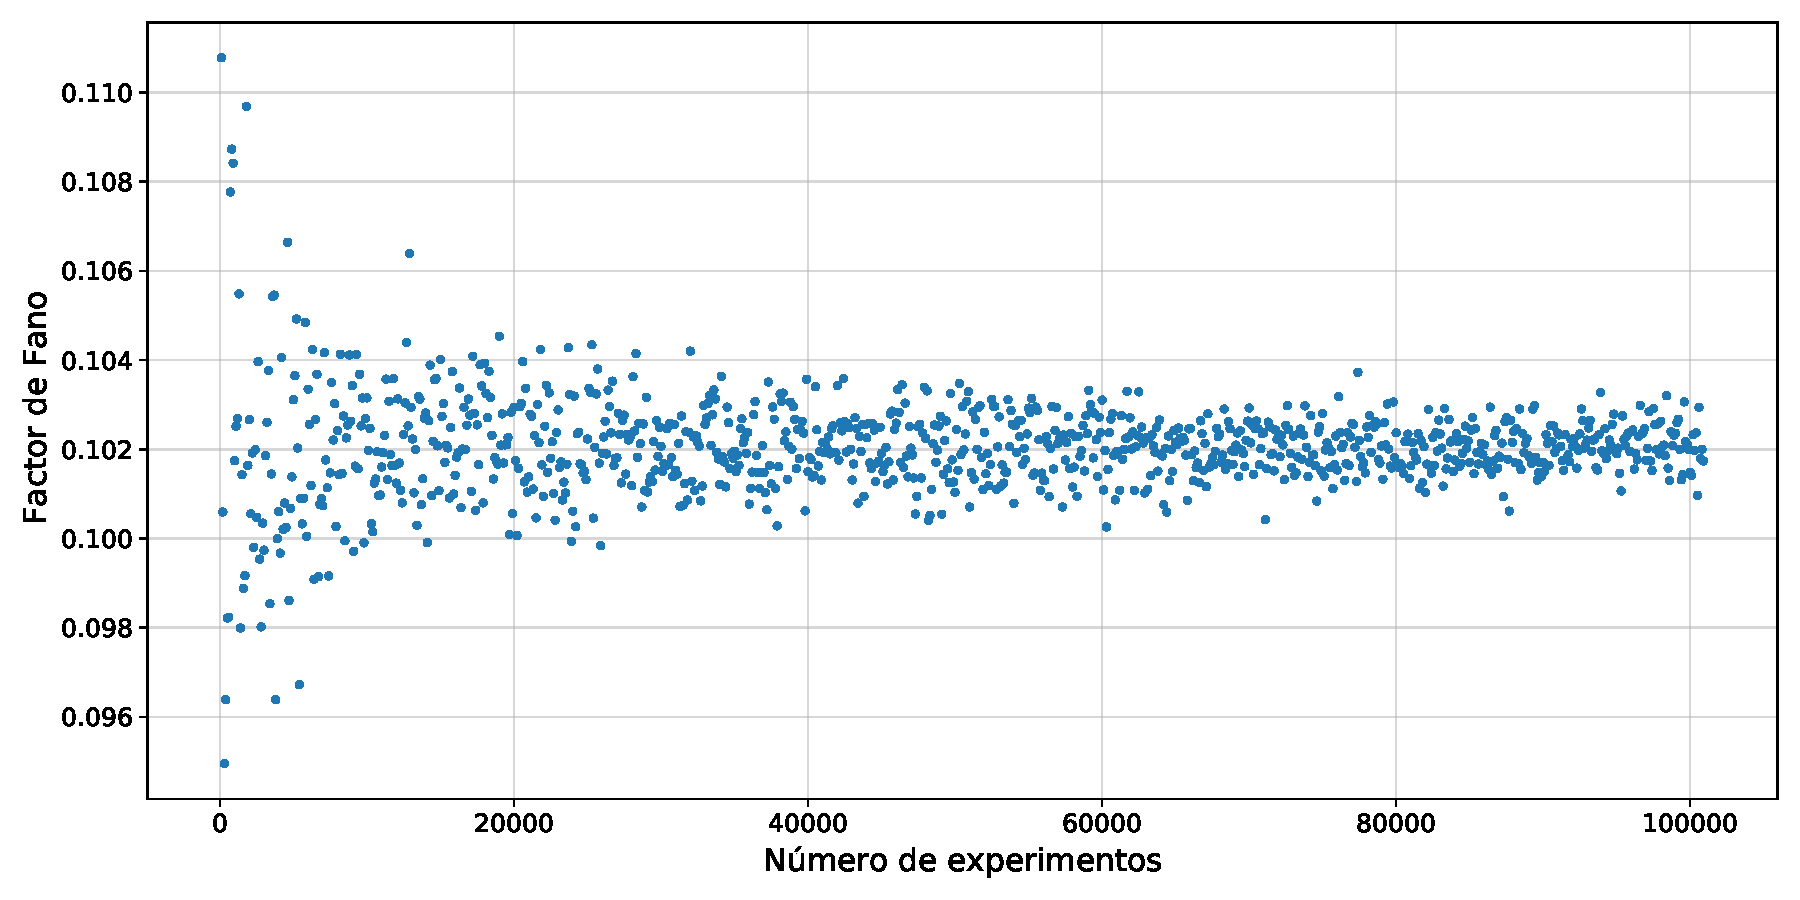
\includegraphics[scale=0.5]{Figs/FanoConvergencia.pdf}
    \caption{\footnotesize{Dispersión de los valores del Factor de Fano cada cantidad de repeticiones del experimento, partiendo desde $100$ repeticiones hasta 100900 repeticiones.}}
    \label{fig:FanoConvergencia}
\end{figure}
Para $10000$ repeticiones se ve que los valores del factor de Fano están acotados entre $\sim 0.106$ y $\sim 0.098$, mientras que para $100000$ repeticiones están acotados entre $\sim 0.104$ y $\sim 0.100$. Se nota claramente la mejora en la estadística.\\
\indent Además, con el fin de poder caracterizar mejor las dependencias entre parámetros en la simulación, se hicieron barridos sobre la pérdida de energía $E_{loss}$ para conocer la dependencia de los resultados respecto de este, partiendo desde $0\,\si{eV}$ de pérdida de energía hasta $7\,\si{eV}$ de pérdida de energía por cada ionización (equivale a perder casi $4$ veces la energía del gap del Silicio). En cada uno se midió el factor de Fano, el valor medio de carga ionizada y la energía de creación electrón hueco, como puede verse en las figuras \ref{fig:FanoVsEloss} \ref{fig:ElossVsMu} y \ref{fig:CreacionHuecoVsEloss}. 
\begin{figure}%[h]
%a) Esta figura se puede hacer con los datos de: fano_Eloss_mu_vec.txt que está en el directorio /home/igna/Escritorio/Tesis2021/Figs/Figuras_Apendice_Simulaciones/txts_para_plots usando el .py Barridos_mu_Eloss_fano.py que está en /home/igna/Escritorio/Tesis2021/Figs/Figuras_Apendice_Simulaciones/pys_para_plots
    \centering
    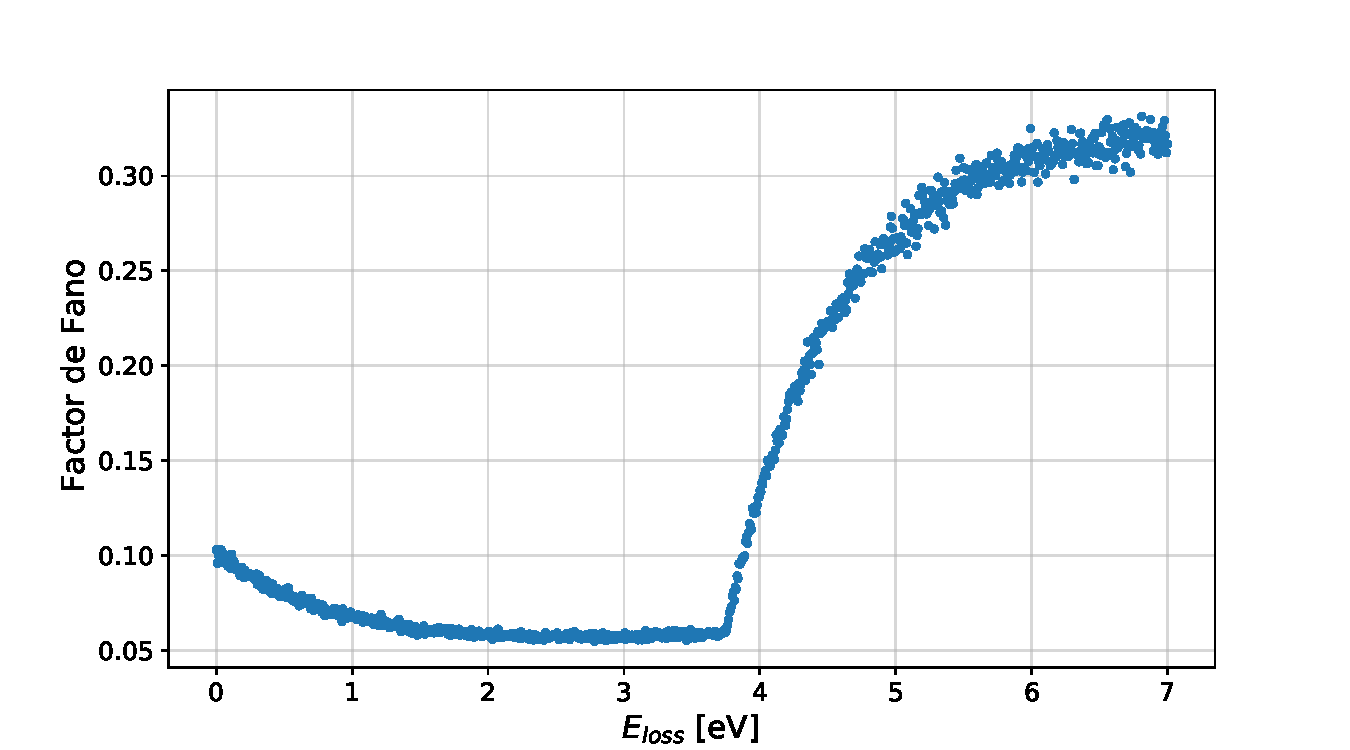
\includegraphics[scale=0.35]{Figs/Fano_vs_Eloss_5ktrials_0-7Eloss.pdf}
    \caption{\footnotesize{asd.}}
    \label{fig:FanoVsEloss}
\end{figure}
La curva del factor de Fano en función de la energía $E_{loss}$ (y al igual que la energía de creación electrón-hueco y el valor medio de carga ionizada) presenta un cambio de régimen abrupto cuando se cruza el umbral $E_{loss} = 3.75\,\si{eV}$. En la figura \ref{fig:FanoVsEloss} puede verse claramente este cambio de régimen. También se observa que cuando hay conservación de la energía, es decir, $E_{loss} = 0$, es cuando se obtiene un factor de Fano más semejante al observado experimentalmente, que está cerca de $0.1$. A medida que aumenta la pérdida de energía, el factor de Fano comienza a decrecer hasta que se alcanza los $3.75\,\si{eV}$ de pérdida de energía, donde se observa el cambio brusco en la curva, y se observa un aumento pronunciado de la misma, semejante a un punto crítico.\\
\indent De la misma forma, el valor medio $\mu$ de la carga ionizada tiene un cambio de concavidad en la curva a medida que aumenta la cantidad de energía perdida por cada ionización, como se ve en la figura \ref{fig:ElossVsMu}.
\begin{figure}%[h]
% b) Esta figura se puede hacer con los datos de: fano_Eloss_mu_vec.txt que está en el directorio /home/igna/Escritorio/Tesis2021/Figs/Figuras_Apendice_Simulaciones/txts_para_plots usando el .py Barridos_mu_Eloss_fano.py que está en /home/igna/Escritorio/Tesis2021/Figs/Figuras_Apendice_Simulaciones/pys_para_plots
    \centering
    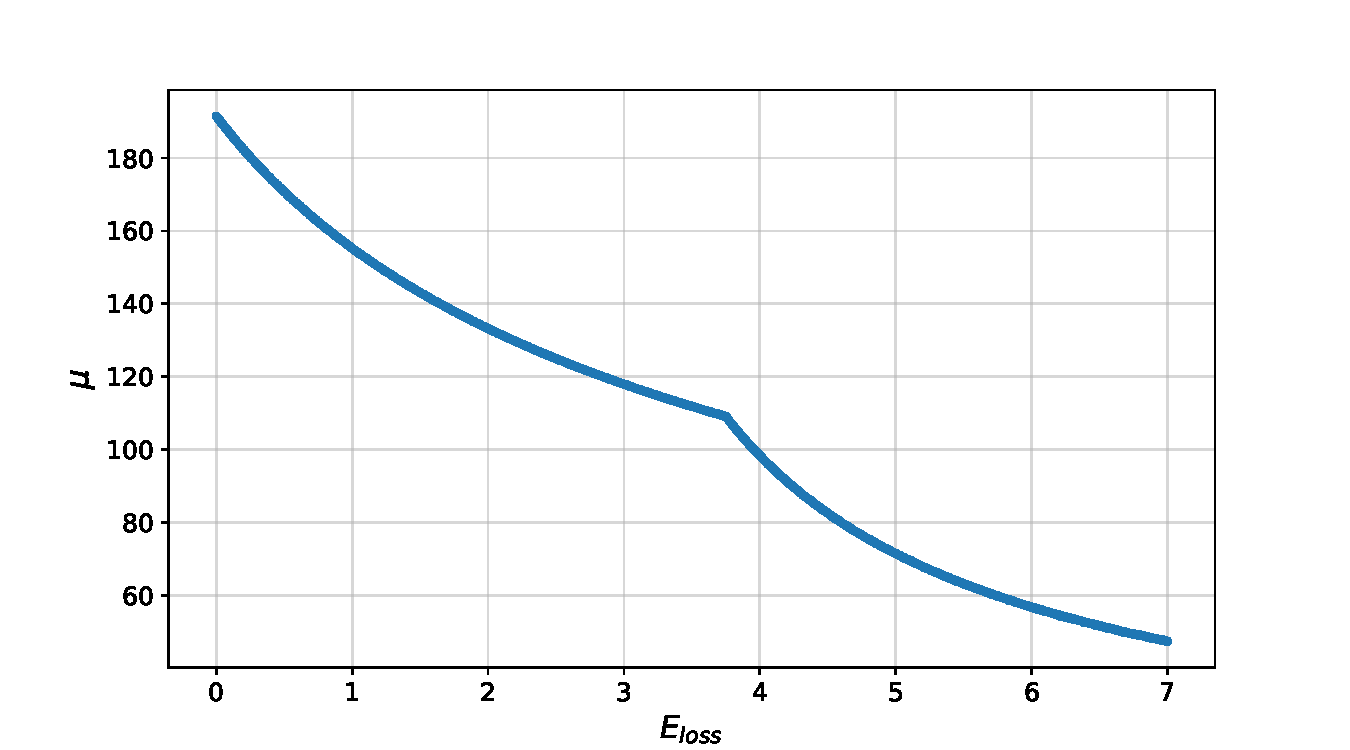
\includegraphics[scale=0.35]{Figs/ELoss_vs_mu_5ktrials_0-7Eloss.pdf}
    \caption{\footnotesize{asd.}}
    \label{fig:ElossVsMu}
\end{figure}
Nuevamente, los valores más cercanos a los medidos experimentalmente son los que corresponden a los casos en los que hay conservación de la energía.\\
\indent Por último, para la energía de creación electrón hueco, calculada a partir del valor medio de carga ionizada y la energía inicial $E_{R} = 677\,\si{eV}$, usando $\left\langle\varepsilon_{\eh} \right\rangle= 677\,\si{eV}/\mu$, claramente tendrá el mismo cambio de régimen en $3.75\,\si{eV}$, como se ve en la figura \ref{fig:CreacionHuecoVsEloss}.
\begin{figure}%[h]
%a) Esta figura se puede hacer con los datos de: fano_Eloss_mu_vec.txt que está en el directorio /home/igna/Escritorio/Tesis2021/Figs/Figuras_Apendice_Simulaciones/txts_para_plots usando el .py Barridos_mu_Eloss_fano.py que está en /home/igna/Escritorio/Tesis2021/Figs/Figuras_Apendice_Simulaciones/pys_para_plots
    \centering
    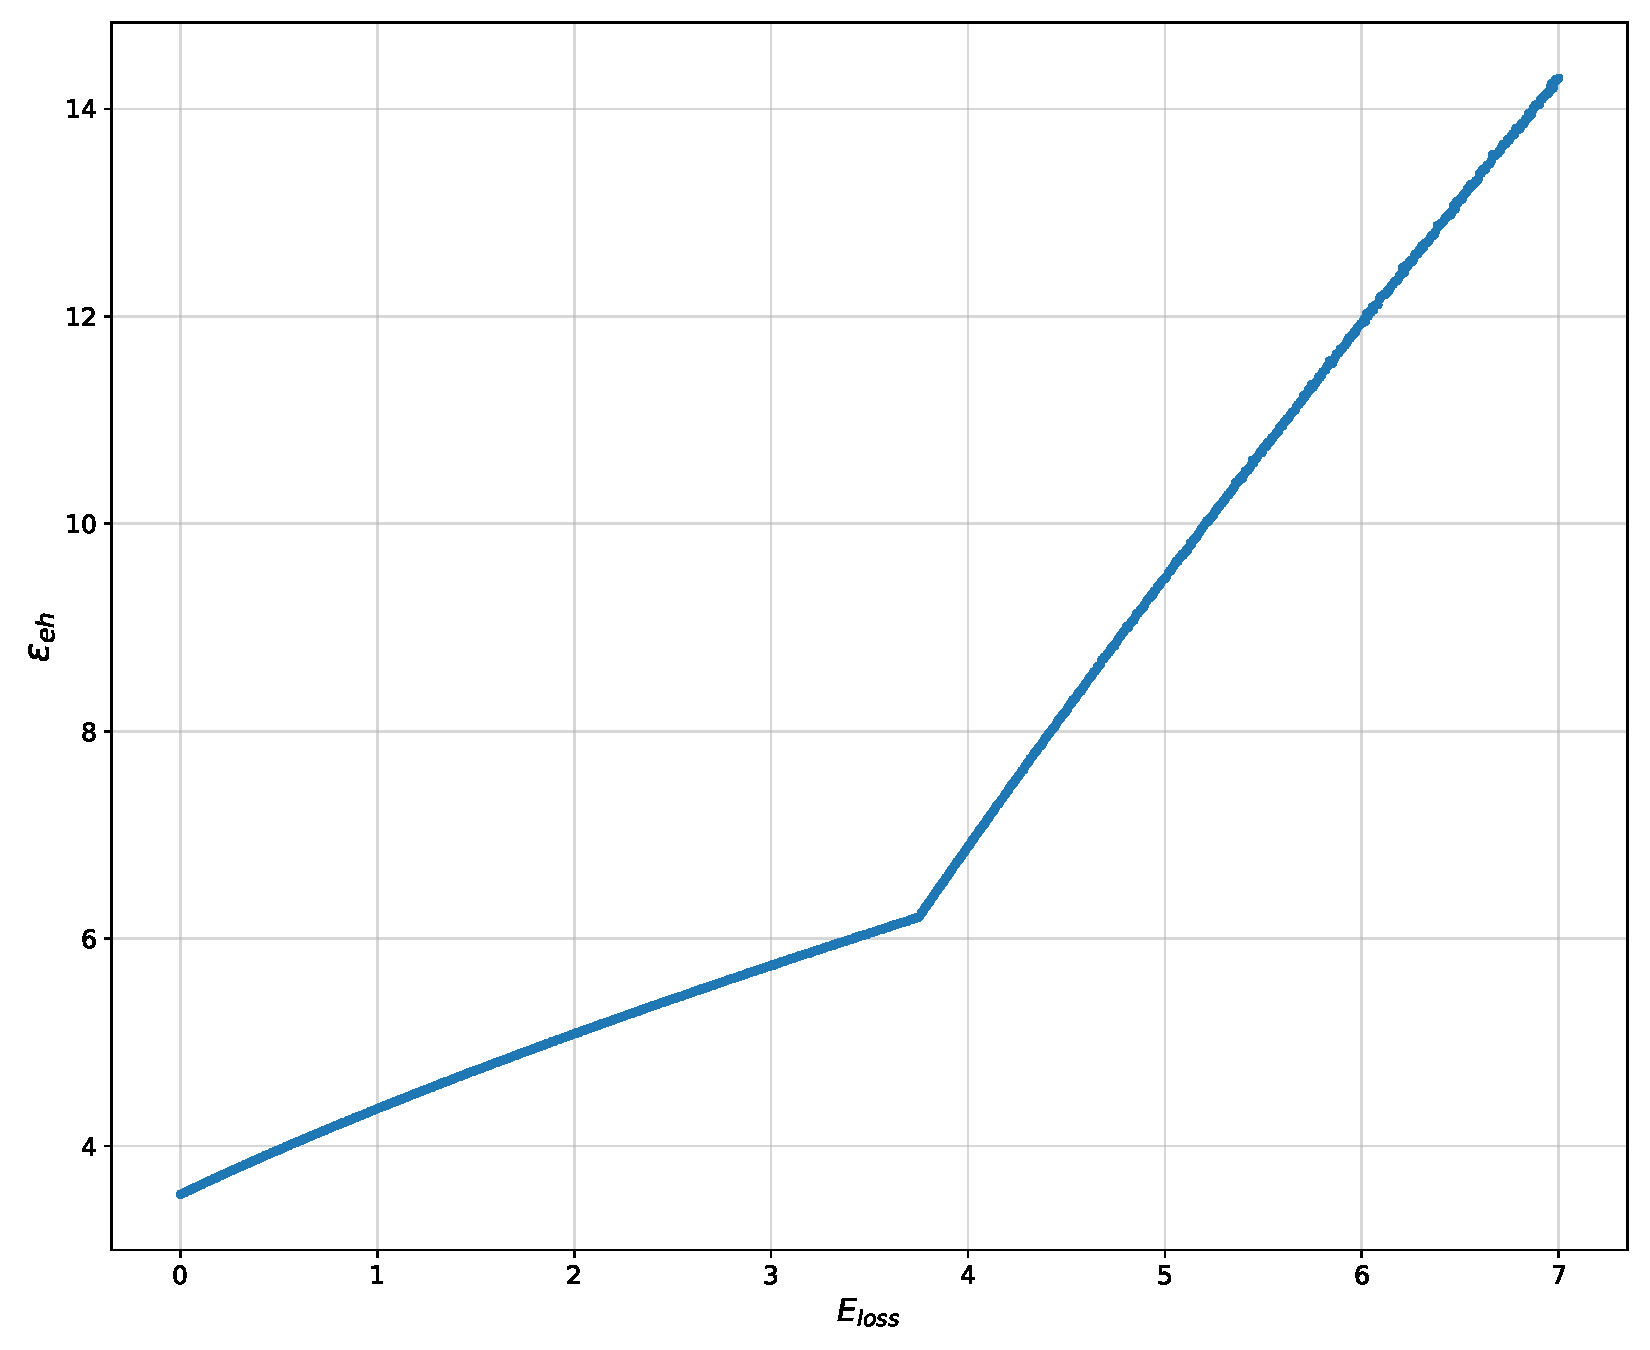
\includegraphics[scale=0.35]{Figs/E_eh_vs_Eloss_5ktrials_0-7Eloss.pdf}
    \caption{\footnotesize{asd.}}
    \label{fig:CreacionHuecoVsEloss}
\end{figure}
Con lo cual se observa que este Monte Carlo es muy sensible a dos parámetros muy importantes de la física real del sistema: La energía de creación electrón hueco, porque es el parámetro que determina si hay o no ionización\footnote{Como se verá en el apéndice}; y la conservación de la energía. Se observa que cuando la energía se conserva en la simulación, se obtienen los resultados más cercanos a los observados experimentalmente y reportados en la bibliografía.\\
\indent Con estos barridos se vio la dependencia de tanto del factor de Fano, como de la energía de creación electrón-hueco y del valor medio de carga ionizada al variar el valor de la energía que se pierde con cada ionización. Se observó que estos parámetros son muy sensibles a la pérdida de energía del sistema, obteniéndose resultados con cambios de regímenes muy pronunciados, particularmente, cuando la energía perdida por ionización coincide con el valor $E_{loss} = 3.75\,\si{eV}$, que casualmente es la energía de creación electrón-hueco promedio y que se usó en la simulación como un parámetro fijo dentro del código\footnote{ver apéndice}.\\
\indent Los resultados de las simulaciones del factor de Fano se ven en los gráficos de las figuras \ref{fig:Simulacion1rden1Fano1} y \ref{fig:Simulacion1rden1Fano2}. Ambos muestran la distribución de carga simulada, un ajuste Gaussiano a ese histograma, usando el $\mu$ y el $\sigma$ generado a partir de los datos y a su vez la forma de la Poissoniana que corresponde a ese valor medio $\mu$. Se ve claramente como la distribución de carga está lejos de parecerse a una distribución de Poisson y por ello el factor de Fano se aleja de la unidad.\\
\indent El primer caso corresponde a una simulación en la que se repitió el mismo experimento de cascada $100000$ veces para tener una buena robustez estadística, mientras que en el segundo caso se usaron $10000$ repeticiones del experimento.\\
\indent En la figura \ref{fig:Simulacion1rden1Fano1} se puede ver lo bien que se ajusta una distribución Gaussiana al histograma. En este caso el factor de Fano correspone a $F = 0.1021$ y el valor medio de carga $\mu = 192$, un valor desplazado a la derecha respecto del valor esperado, cercano a $\mu = 181$.
\begin{figure}%[h]
%Los datos para este gráfico están en /home/igna/Escritorio/Tesis2021/Figs/Figuras_Apendice_Simulaciones/txts_para_plots Distribucion_carga_simulada_100k.txt Para modificar el graf hay que correr el .py que están en /home/igna/Escritorio/Tesis2021/Figs/Figuras_Apendice_Simulaciones/pys_para_plots Fano_100k_dist_carga.py
    \centering
    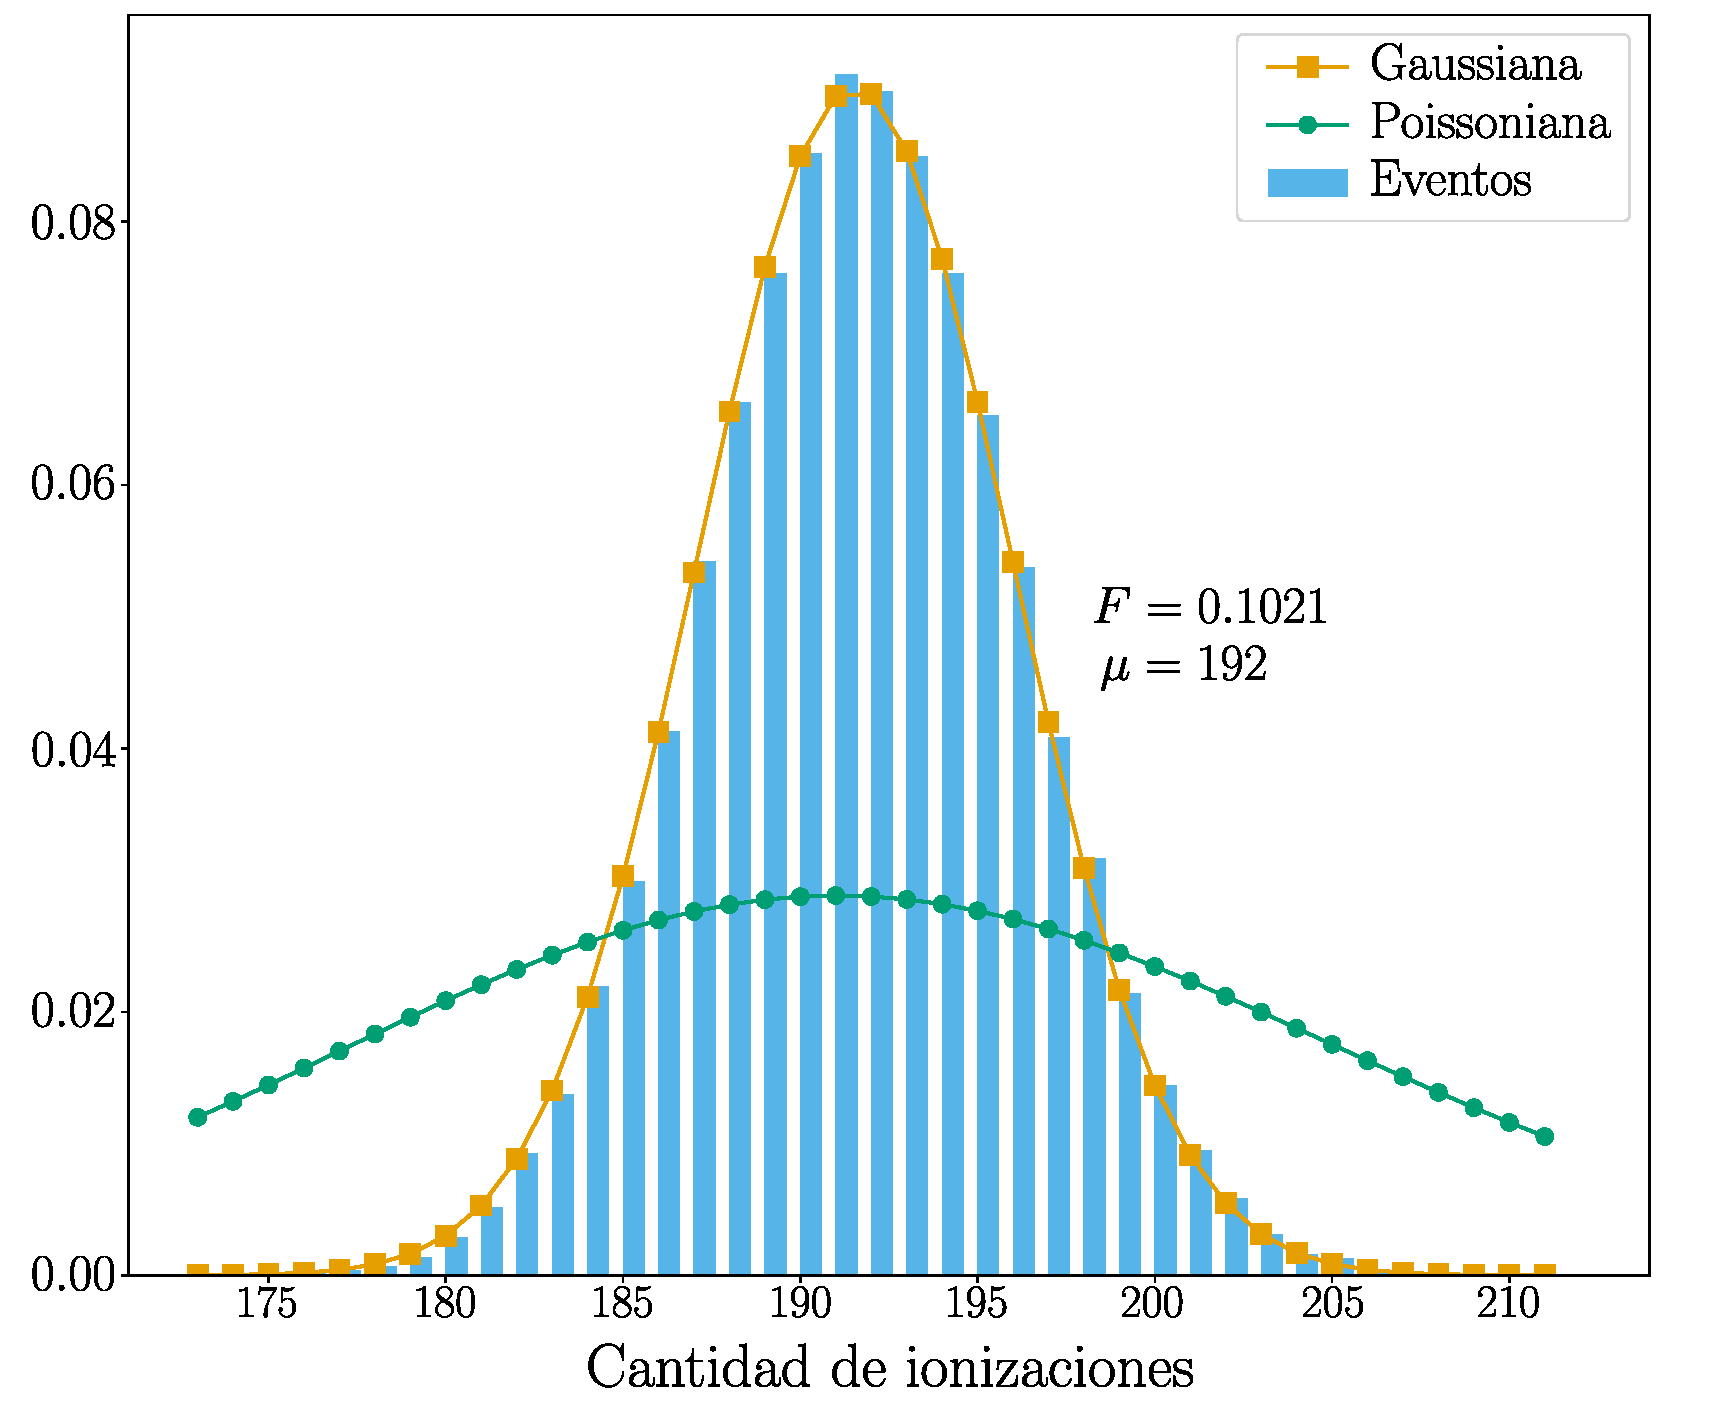
\includegraphics[scale=0.35]{Figs/Fano_677_Eloss0_100ktrials.pdf}
    \caption{\footnotesize{Distribución de carga simulada con el método de Monte Carlo, con parámetro $A = 5.2\,\si{eV}^{3}$ y $100000$ \textit{trials} para obtener la mejor estadística posible. Se observa un valor medio $\mu = 192$, lo cual representa un corrimiento hacia la derecha del valor esperado para el pico de los rayos $X$ del Flúor, que es al rededor de $181$ electrones.}}
    \label{fig:Simulacion1rden1Fano1}
\end{figure}
\noindent Para el segundo caso, en la figura \ref{fig:Simulacion1rden1Fano2}, se modificó el valor del parámetro $A$ de forma que el pico coincida con lo esperado, que son $\mu = 181$ electrones. El valor de $A$ que cumple esa condición es $A = 20\,\si{eV}^{3}$, valor $5$ veces mayor al propuesto en la bibliografía para describir macroscópicamente las propiedades del Silicio.
\begin{figure}%[h]
%Los datos para este gráfico están en /home/igna/Escritorio/Tesis2021/Figs/Figuras_Apendice_Simulaciones/txts_para_plots Distribucion_carga_simulada_10k.txt Para modificar el graf hay que correr el .py que están en /home/igna/Escritorio/Tesis2021/Figs/Figuras_Apendice_Simulaciones/pys_para_plots Fano_10k_dist_carga.py
    \centering
    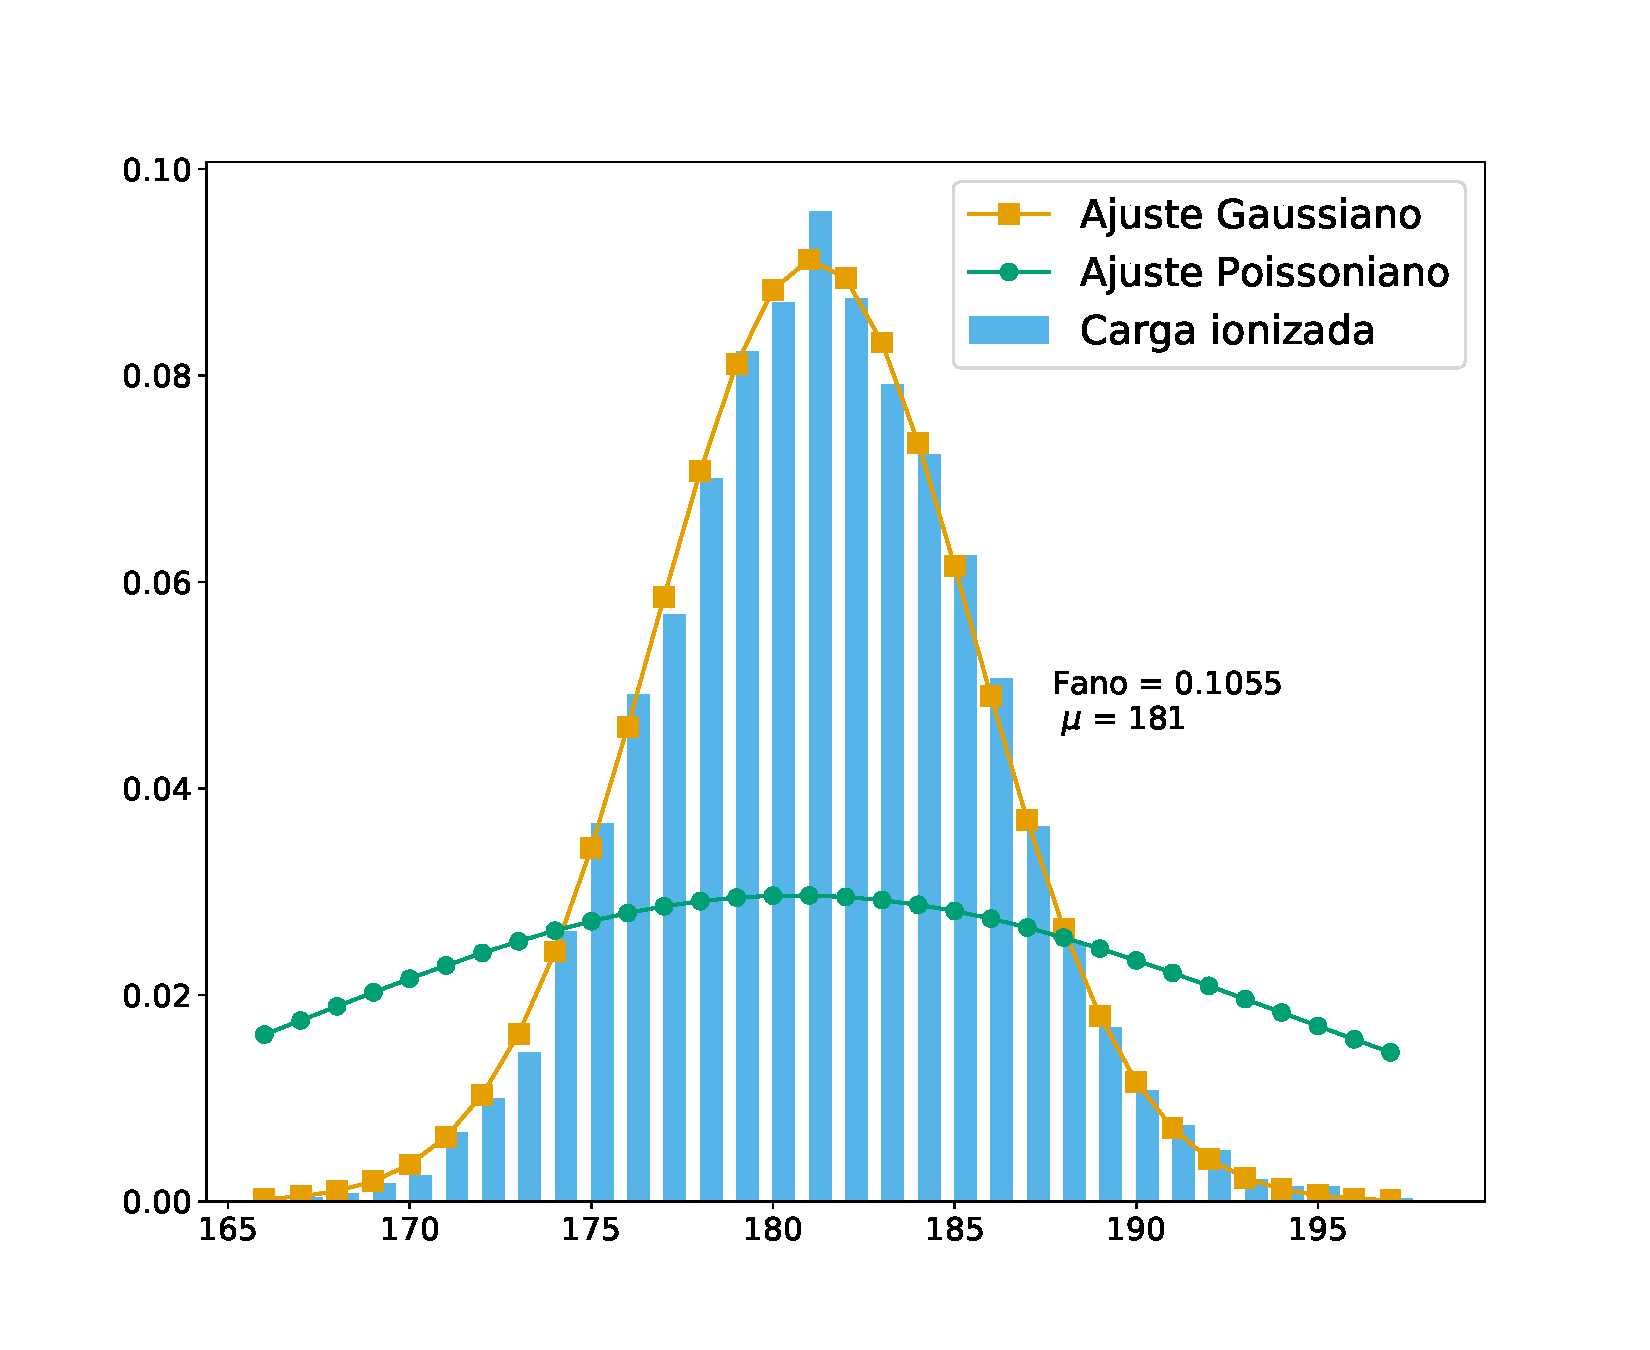
\includegraphics[scale=0.35]{Figs/Fano_677_Eloss0_10ktrials.pdf}
    \caption{\footnotesize{Distribución de carga simulada con el método de Monte Carlo, forzando el parámetro $A$ para que el pico se encuentre en los $181$ electrones esperados para los $677\,\si{eV}$ de energía de los rayos X del Flúor. En este caso $A=20$ y se usaron solamente $10000$ \textit{trials}.}}
    \label{fig:Simulacion1rden1Fano2}
\end{figure}
El factor de Fano en este caso es de $F = 0.1055$, que está contenido entre las bandas esperadas para la cantidad de estadística utilizada en esta simulación. La razón por la cual usar menor estadística en este caso fue porque no era necesaria tanta robustez.\\
\indent En ambos casos el valor del factor de Fano es muy semejante y da, como se esperaba, alrededor de un orden de magnitud inferior a la unidad. Los valores esperados son << buscar valores esperados >>.\\
\indent De estas simulaciones se esperaba poder comprender mejor una de las posibles razones de por qué el factor de Fano es menor a la unidad en las mediciones experimentales. La hipótesis que sustentan estas simulaciones es que el proceso pierde su carácter Poissoniano al depositar toda su energía en el interior del material, ya sea a través de ionización, emisión de fonones u otras pérdidas de energía.

    
    \chapter{El experimento \label{chap:ConfiguracionExperimental}}
%%%%%%%%%%%%%%%%%%%%%%%%%%%%%%%%%%%%%%%%%%%%%%%%%%%%%%%%%%%%%%%%%%
%%%%%%%%%%%%%%%%%%%%%%%%%%%%%%%%%%%%%%%%%%%%%%%%%%%%%%%%%%%%%%%%%%

\noindent En este capítulo se describe el experimento realizado en Fermilab\footnote{Laboratorio Nacional de Aceleradores Fermi en Estados Unidos} para la obtención de los datos utilizados en esta tesis. Si bien el experimento no formó parte de este trabajo, como se verá más adelante, su descripción se vuelve necesaria para explicar algunos de los fenómenos observados.

\section{Configuración experimental}
\noindent Se describe a continuación el sistema utilizado durante el experimento y la estrategia utilizada para obtener los fotones de fluorescencia del flúor y aluminio.

%%%%%%%%%%%%%%%%%%%%%%%%%%%%%%%%%%%%%%%%%%%%%%%%%%%%%%%%%%%%%%%%%%
%%%%%%%%%%%%%%%%%%%%%%%%%%%%%%%%%%%%%%%%%%%%%%%%%%%%%%%%%%%%%%%%%
\subsection{Detector utilizado \label{subsec:detector}}
\noindent El detector utilizado fue un \textit{fully-depleted} CCD, del tipo \textit{back-iluminated}, es decir, que se expone a la radiación incidente uno de sus lados y luego las cargas generadas se migran hacia el lado contrario, teniendo este un espesor total de $200\,\si{\mu m}$. La zona muerta en la parte trasera del CCD estaba compuesta por tres capas: Una capa de $\sim 20\,\si{nm}$ de óxido de indio y estaño (ITO, por sus siglas en inglés: \textit{Indium Tin Oxide}), una capa de $\sim 38\,\si{nm}$ de dióxido de circonio (ZrO$_{2}$) y una última capa de $\sim 100\,\si{nm}$ de dióxido de silicio (SiO$_{2}$). El CCD estaba dividido en cuatro cuadrantes, denominados OHDU, con un amplificador en la esquina de cada cuadrante, permitiendo la lectura en simultáneo de todos ellos. Cada cuadrante consiste en $2063$ filas y $443$ columnas, y cada píxel tiene una dimensión de $15\,\si{\mu m} \times 15\,\si{\mu m}$.

%%%%%%%%%%%%%%%%%%%%%%%%%%%%%%%%%%%%%%%%%%%%%%%%%%%%%%%%%%%%%%%%%%
%%%%%%%%%%%%%%%%%%%%%%%%%%%%%%%%%%%%%%%%%%%%%%%%%%%%%%%%%%%%%%%%%
\subsection{Cámara de vacío}
\noindent El Skipper-CCD se encontraba alojado dentro de una cámara de vacío fabricada a partir de un cubo macizo de aluminio de $20\,\si{cm}$ de lado, denominado \textit{dewar}. El sensor fue operado a $123\,\si{K}$ para disminuir la producción de cargas en el silicio por fluctuaciones térmicas (corrientes oscuras). Para evitar que los fotones infrarrojos emitidos por las paredes de la cámara, que se encontraban a temperatura ambiente, lleguen al detector, este se cubrió con una caja de cobre en contacto térmico con la misma estructura donde se encontraba el detector. 
\begin{figure}[h]
    \centering
    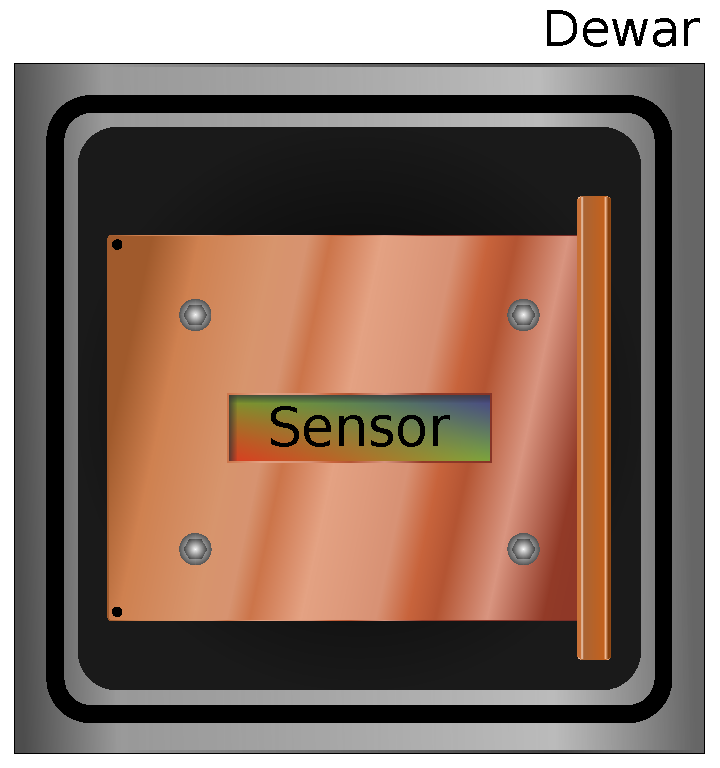
\includegraphics[scale=0.5]{Figs/Frontal_Dewar_Sensor.pdf}
    \caption{Esquema frontal del \textit{dewar} y el posicionamiento del sensor. El sensor se encuentra montado detrás de una placa de cobre con un abertura rectangular por donde la radiación incidente alcanza al sensor. A su vez, se cubren las esquinas laterales del sensor con otras dos láminas de cobre para evitar la exposición de esas regiones del CCD, donde es desplazada la carga para posteriormente ser medida.}
    \label{fig:FrontalDewarYSensor}
\end{figure}
Para evitar la condensación de humedad sobre la superficie del detector debido a las bajas temperaturas, se hizo vacío en el \textit{dewar} mediante la utilización de una bomba turbo-molecular capaz de alcanzar una presión del orden de los $10^{-5}\,\si{mbar}$.

También fue necesaria la utilización de un calentador eléctrico para controlar la temperatura del sensor por dos razones principales: evitar que la temperatura de operación del sensor sea menor a $110\,\si{K}$, debido a que la eficiencia de la transferencia de carga entre píxeles del sensor se ve disminuida para temperaturas menores a esta; y para regular la velocidad de enfriamiento del sensor, dado que podría comprometerse su integridad estructural si esta superaba $1\,\si{K/s}$.

%%%%%%%%%%%%%%%%%%%%%%%%%%%%%%%%%%%%%%%%%%%%%%%%%%%%%%%%%%%%%%%%%%
%%%%%%%%%%%%%%%%%%%%%%%%%%%%%%%%%%%%%%%%%%%%%%%%%%%%%%%%%%%%%%%%%%
\subsection{Fuente de \texorpdfstring{$\Am{241}$}{Am241}}
\noindent En las mediciones estudiadas en este trabajo, se utilizó una fuente radioactiva de $\Am{241}$ electrodepositada, que emitía partículas $\alpha$ con energía de $\sim 5.6\,\si{MeV}$, una actividad de $1\,\si{\mu C}$ y un diámetro de $5\,\si{mm}$. 
Para obtener los rayos $X$ de fluorescencia del flúor y del aluminio, se colocaron dentro de la caja de cobre, frente al sensor, una cinta de Teflón (material que contiene flúor), y una placa de aluminio. La fuente radioactiva se encontraba debajo de esta caja de cobre, a la cual se le hizo un orificio por donde ingresaban las partículas $\alpha$ que impactaban en los materiales mencionados, como muestra el esquema de la Figura \ref{fig:FrontalAlYF}. Esto producía excitaciones en sus nubes electrónicas que luego, al desexcitarse, emitían los fotones de fluorescencia que alcanzaban al sensor.
\begin{figure}[h]
    \centering
    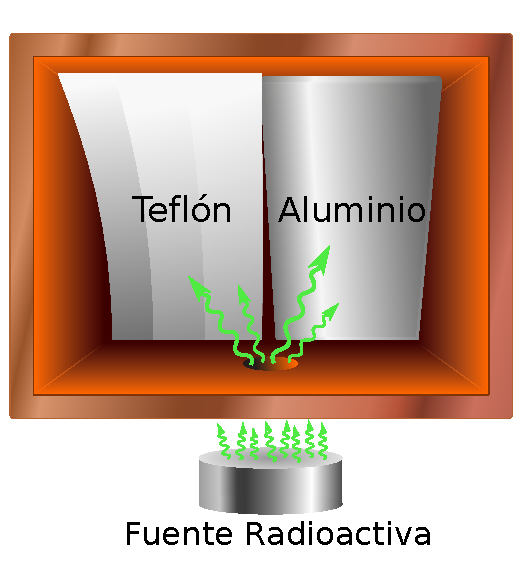
\includegraphics[scale=0.7]{Figs/CajaSensor.pdf}
    \caption{Esquema frontal de la caja de cobre donde se posicionaron la cinta de teflón y la placa de aluminio. Se esquematiza el orificio por donde ingresan las partículas alfa. El sensor se encuentra montado frente de esta, detrás de la placa de cobre del esquema de la Figura \ref{fig:FrontalDewarYSensor}, de forma que los rayos $X$ de fluorescencia producidos por el aluminio y el teflón impacten sobre él.}
    \label{fig:FrontalAlYF}
\end{figure}

En el esquema de la Figura \ref{fig:LateralDewar} puede verse un corte lateral de la cámara. Del lado derecho se encuentra la caja de cobre que contiene el material que se utiliza para producir los rayos $X$ (flúor o aluminio) y la fuente radioactiva emisora de partículas $\alpha$. 
Del lado izquierdo puede verse la estructura que sostiene el detector y la pieza de cobre destinada a regular la temperatura del mismo.

\begin{figure}%[h]
    \centering
    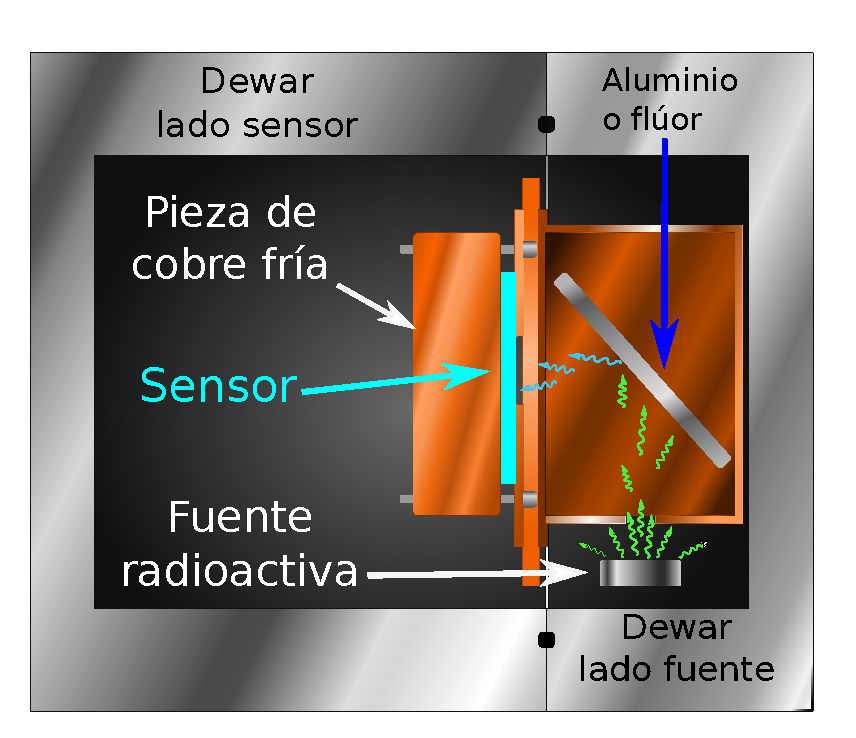
\includegraphics[scale=0.7]{Figs/LateralDewar.pdf}
    \caption{Esquema lateral del \textit{dewar}. Del lado izquierdo se encuentra la placa de cobre con la abertura para el sensor (vista lateral del esquema \ref{fig:FrontalDewarYSensor}) el cual está en contacto con una pieza de cobre fría para mantenerlo a $123\,\si{K}$. Del lado derecho se encuentra la caja de cobre con la pieza de aluminio o de flúor, posicionada en ángulo y por encima del orificio por donde pasan las partículas alfa de la fuente radioactiva (vista lateral del esquema \ref{fig:FrontalAlYF}).}
    \label{fig:LateralDewar}
\end{figure}
Por otro lado, como los fotones de la fuente radioactiva eran capaces de impactar en cualquier parte de la superficie de la caja de cobre, este podría producir también fotones de fluorescencia. Para evitar esto se recubrió el interior de la caja de cobre con cinta \textit{Kapton}, la cual está compuesta por moléculas de bajo número atómico $Z$, que en caso de emitir fotones de fluorescencia, lo harían a energías menores a las estudiadas en este trabajo.
%\textcolor{red}{me quedé con la sensación de que era mejor contar todo esto al revés, primero el sensor, después la fuente radiactiva y por ultimo decir porque se pone la cámara}
%\textcolor{blue}{mover la fuente es más dificil porque hay que reformular y no me parece que amerite}

%%%%%%%%%%%%%%%%%%%%%%%%%%%%%%%%%%%%%%%%%%%%%%%%%%%%%%%%%%%%%%%%%%
%%%%%%%%%%%%%%%%%%%%%%%%%%%%%%%%%%%%%%%%%%%%%%%%%%%%%%%%%%%%%%%%%%

\section{Mediciones \label{sec:Mediciones}}

%\textcolor{red}{hay mucho para mejorar en esta sección que empieza. Varias cosas no son del todo correctas y la explicación no fluye.}\textcolor{blue}{Oka, para mi lo único flojardo es el párrafo que dice "de las $500$ columnas que tiene el sensor, se utilizaron... bla bla" porque eso es lo que no me quedó claro. Pero no veo qué le puede faltar a nivel explicación, yo siento que tiene lo que tiene que tener}

\noindent Las mediciones se realizaron exponiendo la mitad central del sensor a la radiación incidente y dejando las mitades laterales donde se encuentran los amplificadores cubiertos por láminas de cobre, como se ve en el esquema de la Figura \ref{fig:FrontalDewarYSensor}, de forma de evitar su exposición. Los cuatro cuadrantes del sensor son expuestos por un breve período de tiempo a la radiación (decenas de milisegundos), para rápidamente desplazar la carga colectada a la zona del sensor cubierta por las láminas de cobre y evitar que siga recibiendo interacciones durante el proceso de lectura. %, el cual tomaba aproximadamente $11$ minutos.
Este procedimiento es importante porque si no se mueve la carga rápidamente a la región cubierta, la actividad de la fuente saturaría de eventos el detector haciendo imposible la diferenciación de eventos en las imágenes.

%Es importante notar que el tiempo que se demora en desplazar la carga de la región expuesta a la región cubierta depende de la cantidad de columnas del sensor que se quieren medir. Si por ejemplo, quieren medirse $50$ columnas, la columna número $50$ abandonará la región expuesta en un tiempo $t$. Pero si lo que se quiere medir son $100$ columnas, entonces en este caso la columna número $100$ abandonará la región expuesta en un tiempo $\sim 2t$. Esto implica que la cantidad de eventos medidos es proporcional a la cantidad de columnas que se quieran medir además de que las últimas columnas tendrán cada vez más eventos.

%\noindent Debido a que la tasa de eventos de fluorescencia de aluminio y flúor producidos fue relativamente baja, las colección de eventos se realizó exponiendo el detector durante $20$ minutos antes de realizar la medición de la carga en los píxeles. 
Luego, para las mediciones de la carga se utilizaron $300$ muestreos por píxel, que corresponde a un tiempo de lectura de aproximadamente $11$ minutos por imagen. En cada una de ellas fueron utilizadas $50$ filas del sensor, donde para cada una se midieron $500$ píxeles, de los cuales $7$ fueron de \textit{pre-scan}, $50$ de \textit{over-scan} y $443$ de región activa. El \textit{pre-scan} son píxeles adicionales del registro horizontal, cuyo fin es el de proveer un retardo para que la señal de video se estabilice y así poder realizar adecuadamente las mediciones subsiguientes. El \textit{over-scan}, por su parte, también corresponde a píxeles adicionales del registro horizontal: si el registro horizontal cuenta con $443$ píxeles, cuando el primer píxel con carga es desplazado hacia nodo de sensado, quedarán $442$ píxeles con carga por leer y un píxel vacío al final. Este es el primer píxel del \textit{over-scan}. Cuando el segundo píxel con carga es desplazado hacia el nodo de sensado, quedarán $441$ píxeles por leer y 2 píxeles vacíos al final, con lo cual ahora hay 2 píxeles de \textit{over-scan}. De esta forma, a medida que se van leyendo los píxeles de la fila, se van vaciando píxeles al final, que a su vez son desplazados junto con los píxeles con carga hacia el nodo de sensado. Esto hace que el tiempo de exposición a las interacciones de estos píxeles sea mucho menor y, por ende, la probabilidad de capturar carga de estos es muy baja.

%pero cuando se realiza la medición de los píxeles y las cargas son desplazadas secuencialmente, estos se ven obligados a atravesar la región del sensor que está expuesta a la radiación y en consecuencia tienen una probabilidad no nula, aunque muy baja, de colectar algún evento al moverse hacia el nodo de sensado. 

Luego de la lectura, las $300$ mediciones tomadas para cada píxel fueron promediadas y los píxeles del \textit{over-scan}, debido a su baja probabilidad de colectar carga durante el proceso de lectura, fueron usados para calcular y extraer la línea de base de cada fila. Este proceso es necesario en la calibración para poder establecer el valor en ADU's correspondiente al $0$ de carga para cada una de las filas del sensor. 

%Luego de la lectura, las $300$ mediciones tomadas para cada píxel fueron promediadas y los píxeles vacíos del \textit{over-scan} fueron usados para calcular y extraer la línea de base de cada fila. Este proceso es necesario para la calibración, para poder establecer el valor en ADU's correspondiente al $0$ de carga para cada una de las filas del sensor. 

%Las regiones de \textit{pre-scan} y \textit{over-scan} son regiones del sensor que no están colectando carga junto con la región activa, pero cuando se realiza la medición de los píxeles y las cargas son desplazadas secuencialmente, estos píxeles atraviesan la región del sensor expuesta y en consecuencia tienen una probabilidad no nula, aunque muy baja, de colectar algún evento al desplazarse hacia el nodo de sensado. 

%Esa baja probabilidad de colectar carga durante el proceso de lectura es la razón por la cual esos píxeles son utilizadas para definir la línea de base de cada fila. Al final de cada ciclo de exposición/lectura, toda la carga colectada por el CCD era removida en un rápido proceso que toma aproximadamente un segundo.

Las imágenes resultantes luego de la medición y el promediado contienen $50 \times 500$ píxeles por cada cuadrante y la carga es medida en unidades electrónico digitales (ADU's), que posteriormente son convertidas en electrones usando la calibración absoluta del sensor.
    
    \chapter{Caracterización y corrección de sesgos \label{chap:Analisis}}

%%%%%%%%%%%%%%%%%%%%%%%%%%%%%%%%%%%%%%%%%%%%%%%%%%%%%%%%%%%%%%%%%%
\section{Procesado de las imágenes \label{sec:ProcesadoDatos}}
\noindent Los datos obtenidos durante el proceso de medición se almacenan en un tipo de imagen de formato \verb|.fits|. Cada píxel de esa imagen corresponde a la carga medida en el nodo de sensado en ADU's. Si se decidió realizar un número $N$ de muestreos por cada píxel del sensor usando el modo Skipper, entonces la imagen \verb|.fits| producida tendrá $N$ píxeles por cada píxel real del sensor. Por ejemplo, si el sensor estuviera conformado por $16$ píxeles, $4$ filas y $4$ columnas y el número de muestreos elegido fuera de $3$, la imagen resultante tendría una dimensión de $4$ filas por $12$ columnas, como se ve en la Figura \ref{fig:Skipper2root_esquema}. 
Por esta razón, resulta necesario procesar la imagen generada, promediando los $N$ muestreos por píxel y así obtener una lectura de carga con muy bajo ruido a la vez de disminuir drásticamente el tamaño y peso de la imagen.

El procesamiento de las imágenes es llevado a cabo por el programa \verb|skipper2root.exe|, el cual genera una nueva imagen de formato \verb|.fits|, ya promediada y con el tamaño correspondiente a la cantidad total de píxeles del sensor que se utilizaron en la medición. 
A su vez, es este programa el que se encarga de restar la línea de base, utilizando las columnas del \textit{over-scan}, de forma de establecer el valor nulo de carga para cada pixel vacío en las filas del sensor.
\begin{figure}[h]
    \centering
    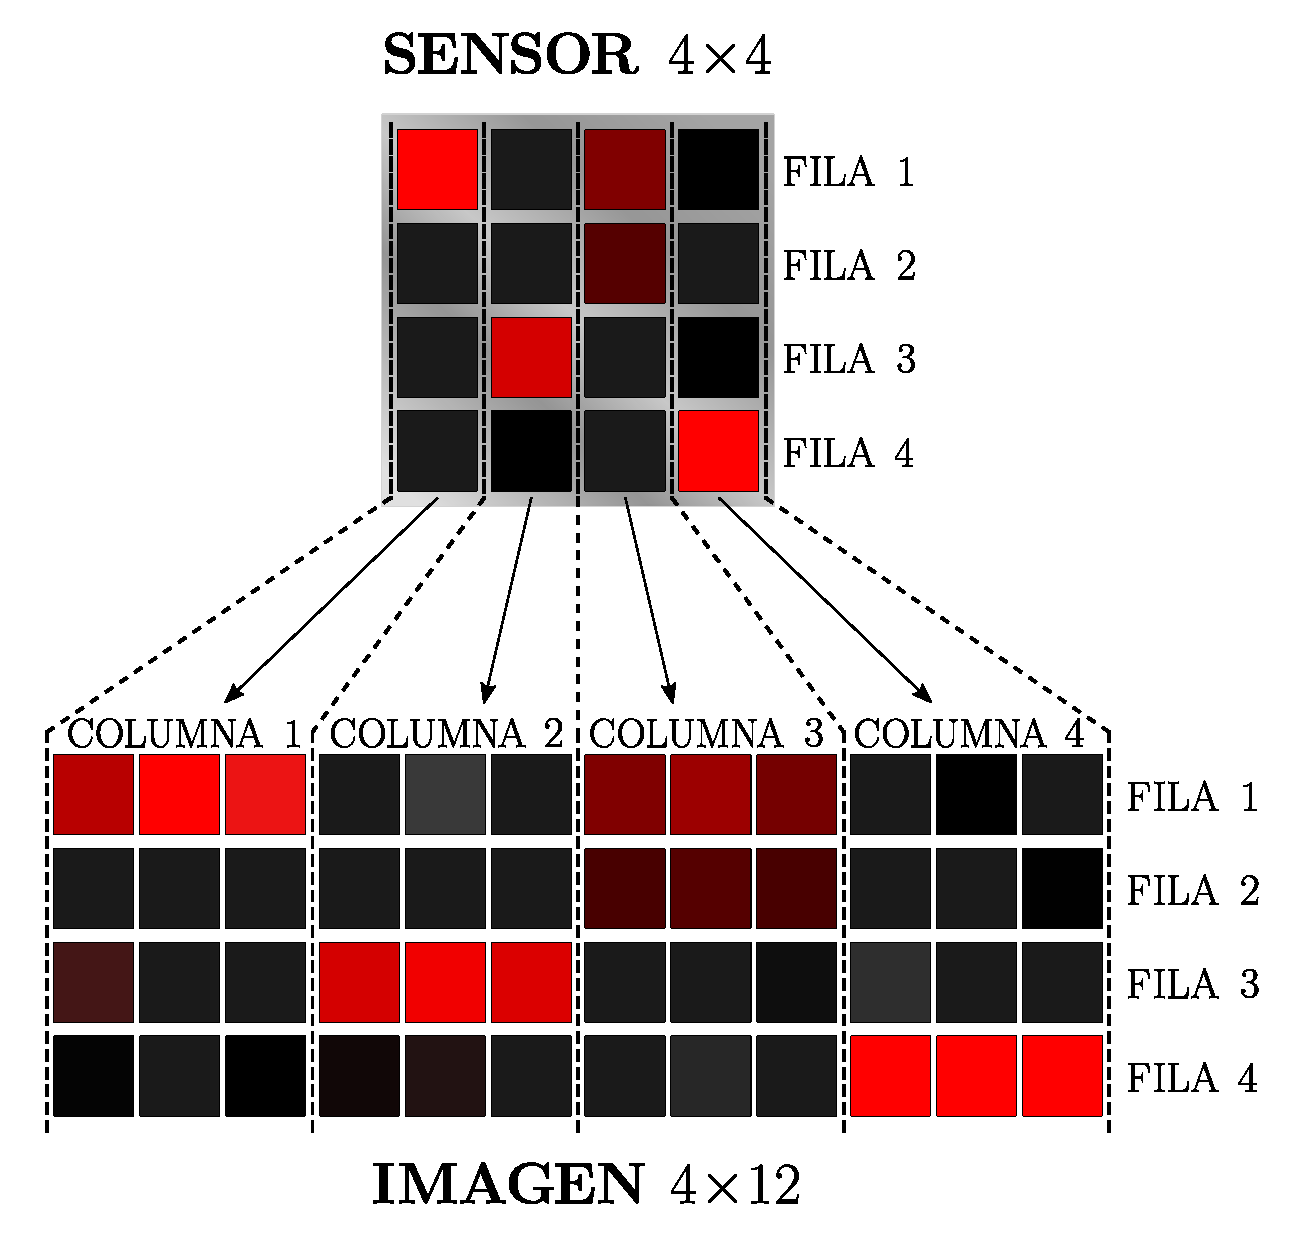
\includegraphics[scale=0.4]{Figs/skipper2root_scheme.pdf}
    \caption{Ejemplo de la imagen obtenida de medir con un sensor de $4\times4$ píxeles utilizando un muestreo de $3$ lecturas por píxel, antes de realizar el promediado de la carga. La imagen resultante es de $4\times 12$ píxeles.}
    \label{fig:Skipper2root_esquema}
\end{figure}

%%%%%%%%%%%%%%%%%%%%%%%%%%%%%%%%%%%%%%%
%\textcolor{red}{Lo que sigue no está en el mejor lugar. La calibración absoluta es algo que nosotros hacemos después de correr skExtract, aca pareciera que es antes.}

% Estas nuevas imágenes tienen la información de la carga de los eventos medidos en cada píxel con ruido subelectrónico gracias al muestreo realizado utilizando el modo Skipper. Sin embargo, los datos en ellas aún están en unidades analógico-digitales (ADUs), con lo cual, para estudiarlas en términos de la cantidad de carga es necesario utilizar una calibración ADU-electrones, que puede obtenerse a partir del método descripto en la Sección \ref{sec:Antecedentes}. Esta calibración se obtiene ajustando un polinomio de orden $4$ de la forma
% \begin{equation*}
%     e^{-} 
%     = \alpha \mbox{ADU} 
%     + \beta \mbox{ADU}^{2}
%     + \gamma \mbox{ADU}^{3}
%     + \delta \mbox{ADU}^{4}
% \end{equation*}
% y es distinta para cada uno de los cuadrantes del sensor, ya que cada uno de ellos cuenta con un amplificador diferente.
%%%%%%%%%%%%%%%%%%%%%%%%%%%%%%%%%%%%%%%

%\textcolor{red}{-----------------------------------------------------------------}

Además, es necesario poder reconocer los conjuntos de píxeles contiguos con carga que pertenecen a un único evento. Con este fin, se utiliza otro programa, el cual hace uso de una calibración lineal para transformar de ADUs a electrones además de reconocer los conjuntos de píxeles con carga por medio de un algoritmo de clusterización. Este programa se llama \verb|skeExtract.exe| y procesa todas las imágenes que \verb|skipper2root.exe| generó para así formar un nuevo tipo de archivo, de formato \verb|.root|, con toda la información de los eventos encontrados en las imágenes. 

Estos nuevos archivos \verb|.root| tienen la información de la carga de los eventos medidos en cada píxel, con ruido subelectrónico gracias al muestreo realizado utilizando el modo Skipper, además de muchos otros parámetros propios de los eventos, como ser la varianza en $x$, varianza en $y$, cantidad de píxeles por cluster, etc.

Algo a tener en cuenta es que la calibración utilizada por \verb|skExtract.exe| es nominal y se realiza solamente para que el archivo \verb|.root| tenga la carga en unidades de electrones, al menos de forma aproximada. Para mejorar la precisión de los análisis que se harán sobre los datos, es necesario volver a calibrar la relación ADU-electrones, y para esto es necesario realizar la calibración absoluta tal como fue descripta en la Sección \ref{sec:Antecedentes}. Esta calibración se obtiene ajustando un polinomio de orden $4$ de la forma
%Sin embargo, los datos en ellas aún están en unidades analógico-digitales (ADUs), con lo cual, para estudiarlas en términos de la cantidad de carga es necesario utilizar una calibración ADU-electrones, que puede obtenerse a partir del método descripto en la Sección \ref{sec:Antecedentes}. Esta calibración se obtiene ajustando un polinomio de orden $4$ de la forma
\begin{equation*}
    e^{-} 
    = \alpha \mbox{ADU} 
    + \beta \mbox{ADU}^{2}
    + \gamma \mbox{ADU}^{3}
    + \delta \mbox{ADU}^{4}
\end{equation*}
sobre los datos y es distinta para cada uno de los cuadrantes del sensor, ya que cada uno de ellos cuenta con un amplificador diferente. Los coeficientes que se obtienen de esta calibración, para cada cuadrante, se guardan en un archivo de formato \verb|.txt|.

Finalmente, se utilizan programas que son los encargados de tomar los archivos \verb|.root| y a partir de estos realizar los análisis estadísticos utilizando \verb|C++| y las librerías para análisis de datos científicos desarrolladas por el CERN llamadas \textit{ROOT}. Esto es, determinar el factor de Fano y la energía de creación electrón-hueco tanto para el flúor como para el aluminio, por medio de un ajuste \textit{no bineado}. Para eso se hicieron dos programas diferentes, uno para cada elemento y se llamaron \verb|Al_Fano_Unbinned_fit.C| y \verb|F_Fano_Unbinned_fit.C|. Estos programas utilizan los coeficientes obtenidos de la calibración absoluta para contar con precisión la cantidad de carga de cada evento. También en ellos se implementan los cortes de calidad que filtran los eventos no deseados y dejan los que se deseen estudiar. Estos cortes de calidad son tanto de forma como de carga: 
\begin{itemize}
    \item Se filtran eventos cuyo tamaño supere cierto radio establecido;
    \item Se filtran eventos cuyas longitudes tanto en $x$ como en $y$ no se encuentren acotadas entre un valor mínimo y un valor máximo, es decir, no se quiere que sean muy largos en alguna dada dirección;
    \item Se filtran eventos cuya carga total no se encuentre comprendida entre un valor mínimo y un valor máximo, de forma de mirar eventos con carga cercana a los de los picos de los rayos $X$ de F o Al.
\end{itemize}
Una vez que se tienen los eventos deseados, el programa realiza los histogramas de carga correspondientes que luego pueden ser usados para realizar un ajuste bineado de los datos. El ajuste bineado consiste en tomar el histograma de carga y ajustar los datos con el modelo utilizado minimizando $\chi^{2}$ para obtener $\mu$, $\sigma$ y $\beta$, donde $\mu$ es el valor medio del pico, $\sigma$ es su dispersión y $\beta$ es un parámetro que da cuenta de la colección parcial de carga, como se verá en el Capítulo \ref{chap:ModeloPCC}. Por otro lado, el ajuste no bineado consiste en tomar los parámetros resultantes del ajuste bineado, inyectarlos en el modelo con el que se desea ajustar y calcular la verosimilitud para todo el conjunto de datos. En este caso, se fija el valor de $\beta$ y se dejan libres $\mu$ y $\sigma$ que son variados hasta que se maximiza la verosimilitud. Los parámetros que maximicen la verosimilitud serán los parámetros óptimos para el ajuste. La necesidad de utilizar un ajuste bineado previamente para calcular los parámetros surge de que favorece la velocidad de convergencia del ajuste no bineado.

A partir del análisis de las imágenes previamente descripto se obtienen: el factor de Fano, la energía de creación electrón-hueco y el espesor de la zona de colección parcial de carga.

%%%%%%%%%%%%%%%%%%%%%%%%%%%%%%%%%%%%%%%%%%%%%%%%%%%%%%%%%%%%%%%%%%
\section{Impacto del corte propuesto}
\noindent En este trabajo se propone analizar un conjunto de imágenes, eliminando los eventos de un electrón presentes en ellas. Se trabaja sobre la hipótesis de que esto deberá incrementar el conteo de eventos con la cantidad de carga deseada y se espera que esta mejora en la estadística redunde en mayor precisión en la determinación de las cantidades de interés. Sin embargo, aplicar este corte trae aparejado un sesgo en el conteo de carga de cada evento que debe corregirse.

Es pertinente entonces cuantificar el aumento en la estadística al realizar el corte mencionado y así motivar el análisis en busca de una mejora en el cálculo de las incertezas de las cantidades de relevancia para este trabajo.

El parámetro clave para llevar esto a cabo se llama \verb|EPIX| y es un valor umbral que define a partir de qué cantidad de carga en un píxel se cuenta o no como un píxel vacío. El mismo forma parte del programa de reconocimiento de clusters (\verb|skeExtract.exe|). Por ejemplo, para \verb|EPIX=0.5|, todos los píxeles con carga menor o igual a $0.5$ se cuentan como píxeles vacíos, y los que tengan carga mayor a $0.5$ serán contabilizados normalmente; para \verb|EPIX=1.5|, todos los píxeles con carga menor o igual a $1.5$ se cuentan como píxeles vacíos y los píxeles con carga mayor a $1.5$ se cuentan normalmente. En la Figura \ref{fig:HistogramaEPIX} puede verse un esquema de un histograma de los niveles de carga y dónde se sitúa el umbral \verb|EPIX| para realizar el corte.
\begin{figure}[h]
%Como reproducir este gráfico: correr el script NivelesOcupacionCargaEPIX_e.py ubicado en /Escritorio/Tesis2021/Figs/pys_para_plots y buscar la imagen en /home/igna/Escritorio/Tesis2021/Figs/
    \centering
        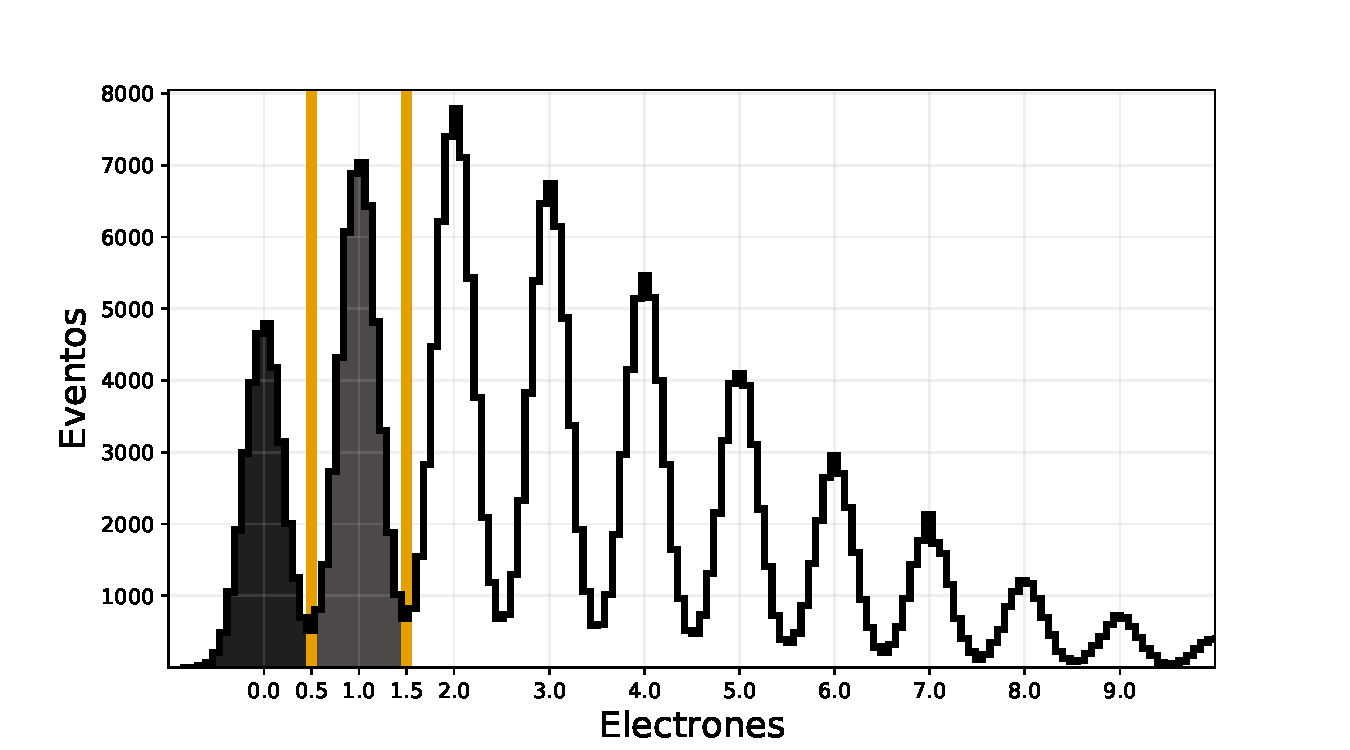
\includegraphics[scale=0.5]{Figs/EsquemaEPIX_histocarga.pdf}
    \caption{Histograma de los datos obtenidos al iluminar el CCD con LED, correspondiente a una región con poca ocupación, donde se han marcado con dos rectas verticales los umbrales para \texttt{EPIX=0.5} y \texttt{1.5}. Depende de cuál umbral sea usado, toda la carga que se encuentra a la izquierda del umbral se considera nula.}
    \label{fig:HistogramaEPIX}
\end{figure}

En el trabajo predecesor de esta tesis\cite{TesisKevin}, los valores obtenidos para el factor de Fano y energía de creación electrón-hueco, fueron calculados utilizando un valor de \verb|EPIX=0.5|. Se espera que al modificar este parámetro, el número de eventos varíe y que, en particular, aumente cuando el \verb|EPIX| aumenta. Esto se debe a que es muy común que se tenga un evento de interés, por ejemplo un cluster de $4$ píxeles de área con una carga total de $180$ electrones (para el caso del flúor) y alrededor de este se acumulen píxeles con fondo de, por ejemplo, $1$ o muy raramente $2$ electrones. En estos casos podría suceder que la conexión entre estos clusters y los píxeles con carga espuria se extienda lo suficiente como para que el algoritmo reconozca un gran cluster con exceso de carga y sea desechado por el programa dado que no cumple con los cortes de calidad impuestos. También podría suceder que estos píxeles con carga espuria conecten dos de estos clusters, lo cual es un caso más extremo, dado que el algoritmo reconocería un único cluster de $\sim 360$ electrones, de forma que se perderían, no uno, sino dos eventos que podrían aportar positivamente a la estadística. Al aplicar un umbral que elimine los píxeles con carga espuria que se amontonan y/o conectan con clusters, el programa es capaz de diferenciar y contar los eventos correctamente.

En la Figura \ref{fig:ClusterPegoteado} se muestra un ejemplo de un evento de $179$ electrones para una medición con flúor, que es un evento de interés que el programa debería reconocer, y que hasta que no se eliminan los eventos de un electrón de la imagen, el programa lo identifica como un gran cluster con aproximadamente $40$ electrones más de carga y sin una forma definida (imagen central, píxeles pintados de blanco). A la derecha la imagen con el cluster individualizado y reconocido correctamente por el algoritmo al eliminar la carga excedente.
\begin{figure}[H]
%Para modificar este plot hay que ir a Escritorio/Tesis2021/Figs/pys_para_plots y modificar clusters_no_pegoteados.py
    \centering
    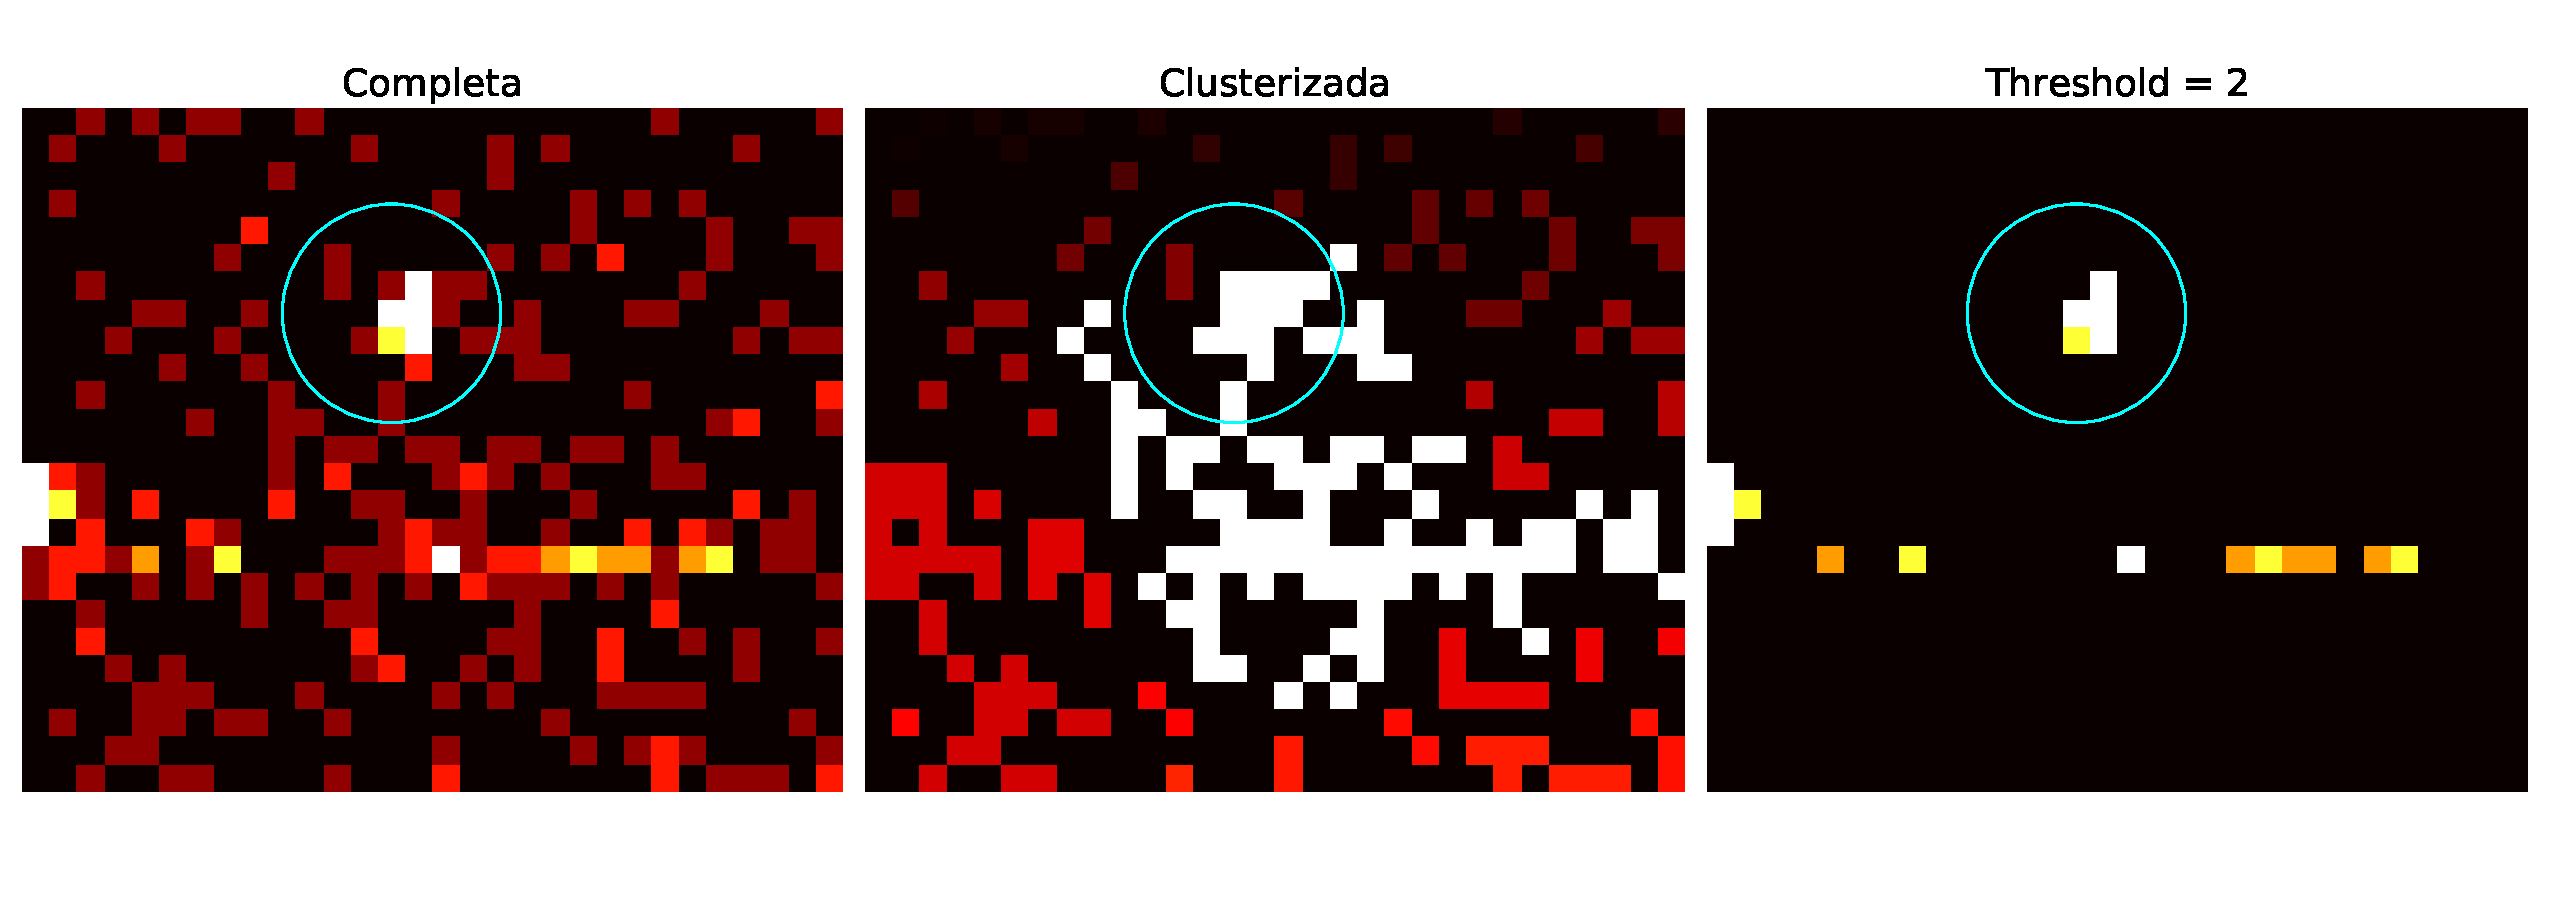
\includegraphics[scale=0.4]{Figs/despegoteo_clusters.pdf}
    \caption{Ejemplo del caso de un evento cercano a los $180$ electrones de carga, que son los eventos buscados. En la imagen de la izquierda se ve la medición sin alterar (ya convertida a unidades de carga). En la imagen del centro se ve en blanco y en un degrade muy tenue de rojos los diferentes clusters que el algoritmo logra reconocer. Lo importante de esta imagen es notar que el algoritmo reconoce como un único cluster (blanco) a un número de píxeles muy grande debido justamente a que píxeles con una única carga generan la unión entre todos ellos. Por último, la imagen de la derecha contiene el cluster de interés una vez que los eventos de un electrón son desechados del análisis, haciendo que pueda contabilizarse correctamente.}
    \label{fig:ClusterPegoteado}
\end{figure}
%En este punto es importante entender cuáles son los sesgos que afectan el conteo de carga de los eventos y para esto es necesario hacer algunas definiciones: se entiende por cluster a todo conjunto de píxeles contiguos con carga mayor o igual a uno que el algoritmo de clusterización es capaz de reconocer en las imágenes. Se define como superficie del cluster al conjunto de píxeles contiguos con carga mayor o igual a uno que pertenecen a un único evento de interés y que no tienen fondo. Nótese que no es posible conocer exactamente la superficie de un cluster. Por último, se define como borde del cluster a todos aquellos píxeles que de no existir fondo se encontrarían vacíos alrededor de la superficie de un cluster. 

En este punto es importante entender cuáles son los sesgos que afectan el conteo de carga de los eventos. En principio, el fondo puede añadir carga extra a la carga real de un cluster proveniente de un evento de interés, generando un corrimiento hacia la derecha en los picos de los espectros. Este caso puede dividirse en dos
\begin{itemize}
    \item La carga extra que puede añadirse a los píxeles interiores (o de superficie) de un cluster.
    \item La carga extra que puede añadirse a los píxeles, inicialmente vacíos, inmediatamente contiguos a los píxeles de superficie de un cluster (caso apreciable en la Figura \ref{fig:ClusterPegoteado}).
\end{itemize}

Sin embargo, la aplicación del umbral (o del corte) modifica estos sesgos. Debido a que este corte elimina todos los píxeles con un electrón, aquellos que inicialmente estaban vacíos pero se agregaron al cluster por efecto de fondo, ahora son eliminados (y con ellos, el segundo caso mencionado anteriormente). Pero también es posible que se eliminen píxeles con un electrón de carga que sí pertenecen a un cluster, %(tanto de la superficie como del borde),
por lo tanto, una vez aplicado el corte, los sesgos se resumen en:
\begin{itemize}
    \item La carga extra que puede añadirse a los píxeles interiores (o de superficie) de un cluster debido al fondo.
    \item La eliminación de píxeles con un único electrón que genuinamente pertenecían a un cluster debido al corte.
\end{itemize}

Se llevó a cabo entonces el análisis de las imágenes obtenidas al exponer el CCD a los rayos $X$ del flúor, con diferentes valores de umbral de corte: \verb|EPIX=0.5|, \verb|EPIX=1.5| y \verb|EPIX=2.5| y se comparó con los resultados obtenidos para el conteo total de eventos. 
Debe tenerse presente que estos son resultados preliminares, ya que el sesgo añadido por la aplicación del umbral al conteo de carga será posteriormente corregido.

Esto se hizo para tres de los cuatro cuadrantes del sensor y para la suma de estos, dado que el segundo cuadrante no funciona correctamente. En el gráfico de la Figura \ref{fig:EntradasVsEpix} se observa un drástico aumento en la cantidad de entradas (eventos contabilizados) cuando se varía el \verb|EPIX|.
\begin{figure}[h]
%Para hacer estas figs hay que ir a /home/igna/Escritorio/Tesis2021/Figs/pys_para_plots y correr plots_entries_fano_eh.py que usa los datos que están en /home/igna/Escritorio/Tesis2021/Figs/txts_para_plots y se llaman Entries_count.txt
    \centering
    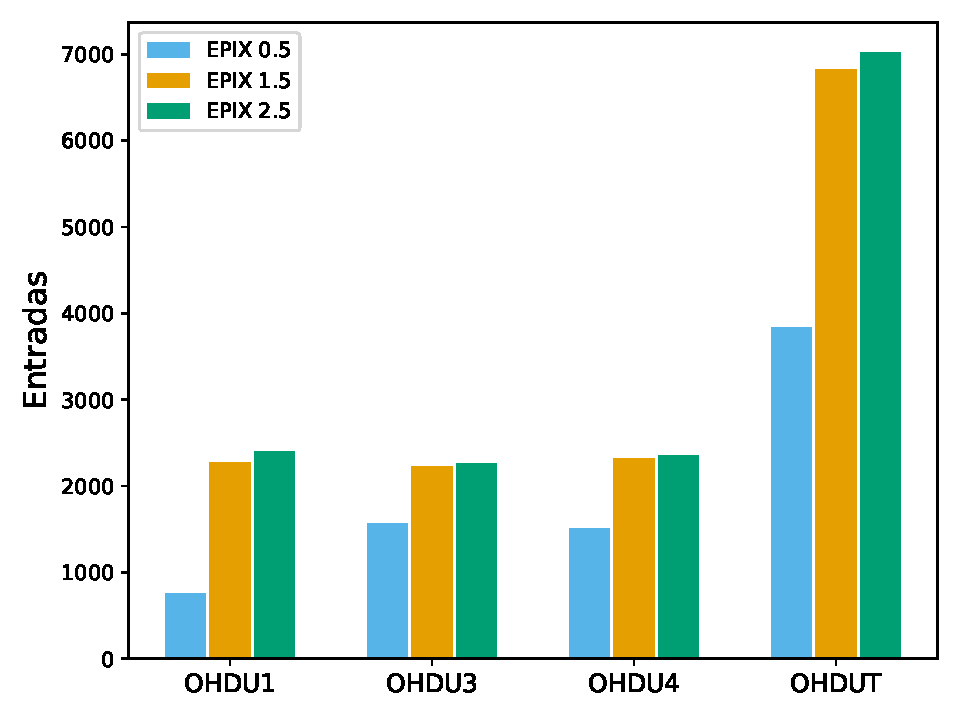
\includegraphics[scale=0.5]{Figs/Entradas_vs_Epix.pdf}
    \caption{Gráfico de barras para la diferente cantidad de entradas contabilizadas por el programa, tanto para valores diferentes de EPIX como para los diferentes cuadrantes del sensor. OHDUT hace referencia a la suma de las entradas del resto de los cuadrantes funcionales ($1$, $3$ y $4$). Se observa un aumento de más del doble en la cantidad de entradas para el primer cuadrante, y un aumento importante pero menos pronunciado para el resto de los cuadrantes.}
    \label{fig:EntradasVsEpix}
\end{figure}
Se puede ver como los cuadrantes $1$, $3$ y $4$ tienen un cambio pronunciado en la cantidad de entradas al pasar de \verb|EPIX=0.5| a \verb|EPIX=1.5| como se esperaba, mientras que al pasar de \verb|EPIX=1.5| a \verb|EPIX=2.5| el aumento es mucho menos pronunciado. 
Particularmente, es el primer cuadrante el que registra el mayor incremento en la cantidad de entradas en relación a los otros. 

En la Tabla \ref{tab:EntriesVsEpix} se presentan los valores precisos del cambio en el número de entradas para cada cuadrante y para cada valor de \verb|EPIX|. 
El primer cuadrante pasa de tener $760$ entradas para \verb|EPIX=0.5| a tener $2272$ para un \verb|EPIX=1.5|, casi el triple, es un aumento de $\sim 198\%$. En cambio, los cuadrantes $3$ y $4$ pasan de tener $1571$ y $1503$ entradas a $2229$ y $2320$, un aumento muy similar y en torno al $\sim40\%$ y $\sim50\%$ respectivamente.
\begin{table}[h]
\centering
\begin{tabular*}{\textwidth}{c @{\extracolsep{\fill}}ccccc}%{@{}ccccc@{}}
\toprule
           & OHDU 1 & OHDU 3 & OHDU 4 & OHDU 1 + 3 + 4 \\ \hline\hline
EPIX = 0.5 & 760    & 1571   & 1503   & 3834           \\
EPIX = 1.5 & 2272   & 2229   & 2320   & 6821           \\
EPIX = 2.5 & 2399   & 2261   & 2356   & 7016           \\ \bottomrule
\end{tabular*}
\caption{Diferentes valores para las entradas, para cada uno de los cuadrantes, para los diferentes valores de EPIX utilizados.}
\label{tab:EntriesVsEpix}
\end{table}

Habiendo tomado este rumbo, es necesario poder remover el sesgo producido por la eliminación de carga en los eventos medidos al aplicar este umbral. Si bien este proceso genera un aumento en la estadística, también genera un corrimiento hacia la izquierda en los picos de los espectros que debe ser corregido. Además, también es necesario remover el exceso de carga que tengan los clusters de debido al fondo presente en las imágenes y que en este caso genera un corrimiento a la derecha de estos picos. En adelante, la idea es intentar comprender este fondo en las imágenes y con ello poder aplicar correcciones a los valores de carga de los clusters, una vez aplicado el umbral y así mejorar la incerteza de los resultados.

%%%%%%%%%%%%%%%%%%%%%%%%%%%%%%%%%%%%%%%%%%%%%%%%%%%%%%%%%%%%%%%%%%
\section{Caracterización de las imágenes}
\noindent Todo el análisis cuantitativo anteriormente descripto se realizó sin la necesidad de inspeccionar visualmente las imágenes de las cuales se extraen los datos. Simplemente se aplicaron diferentes umbrales de prueba y se contabilizó el aumento en la estadística. Sin embargo, ver las imágenes y rápidamente poder reconocer patrones, como exceso de eventos en una misma región para diferentes imágenes o cualquier característica que visualmente sea reconocible pero que al analizar los datos de forma automatizada pueda quedar ofuscada, es un factor importante a la hora del estudio de los datos. Dado que la cantidad de imágenes utilizadas en este trabajo es superior a las $900$, observar una por una es una tarea monumental e impracticable. Por esta razón fue necesario buscar maneras de poder extraer información contenida en todas las imágenes, de forma práctica y realizable, como por ejemplo, generar una imagen \textit{promedio}. Con este fin, se hizo un análisis visual, cualitativo y cuantitativo de las imágenes para comprender mejor los datos, explorar las características del sensor y de cada uno de sus cuadrantes y poder reconocer posibles deficiencias o particularidades relevantes.

Uno de los primeros factores a caracterizar tiene que ver con la carga de los píxeles que no es debida a eventos de interés. Estos pueden ser producto de corrientes oscuras (electrones que sufren excitaciones espontáneas debido a fluctuaciones térmicas del sensor), rebotes de un fotón de baja energía en las paredes de la cámara de vacío donde se encuentra el sensor, etc. No es sencillo y no existe una única manera de estimar el fondo en un sensor, por lo que se ensayaron diferentes maneras de encarar este análisis.

Lo primero que se hizo fue buscar la manera de explorar solamente los píxeles que tuvieran una única carga. Asumiendo que en la gran mayoría de los casos, los píxeles con una única carga que se encuentran aislados de otros píxeles o de clusters de interés, son eventos que forman parte del fondo del sensor, es natural empezar el análisis con estos. Una forma de caracterizar esto es tomar las imágenes y extraer todos los píxeles donde la carga sea mayor que un electrón. De este modo, se obtienen imágenes donde solo hay eventos de un electrón y todo lo demás son píxeles vacíos. En la Figura \ref{fig:ImagenFitsOriginal} se puede ver una típica imagen tomada con el sensor, para el primer cuadrante, en la que claramente pueden observarse algunos eventos muy brillantes y un intenso fondo. En la imagen \ref{fig:ImagenFits1e} en cambio puede verse la imagen resultante de extraer todos los píxeles cuya carga es mayor a un electrón.
\begin{figure}[h]
%Para hacer estas figs hay que ir a /home/igna/Escritorio/Tesis2021/Figs/pys_para_plots y correr imagenes_fits_original_y_filtrada.py
    \centering
    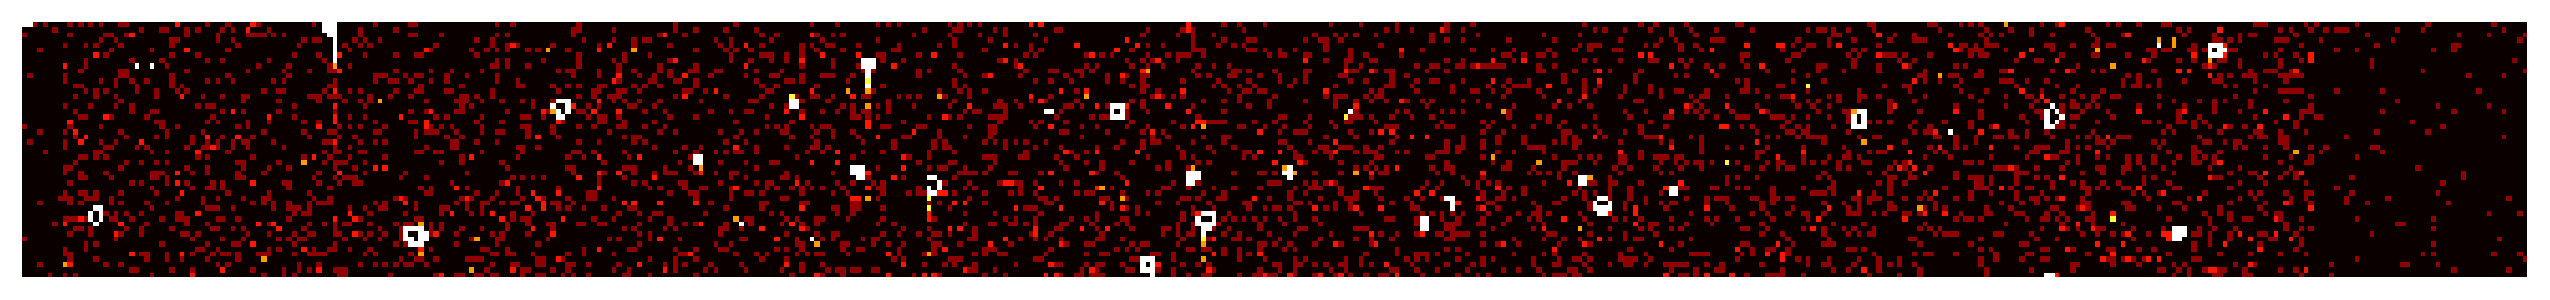
\includegraphics[scale=0.4]{Figs/imagen_fits_original.pdf}
    \caption{Ejemplo de imagen tomada con el sensor, en el primer cuadrante.}
    \label{fig:ImagenFitsOriginal}
\end{figure}

\begin{figure}[h]
%Para hacer estas figs hay que ir a /home/igna/Escritorio/Tesis2021/Figs/pys_para_plots y correr imagenes_fits_original_y_filtrada.py
    \centering
    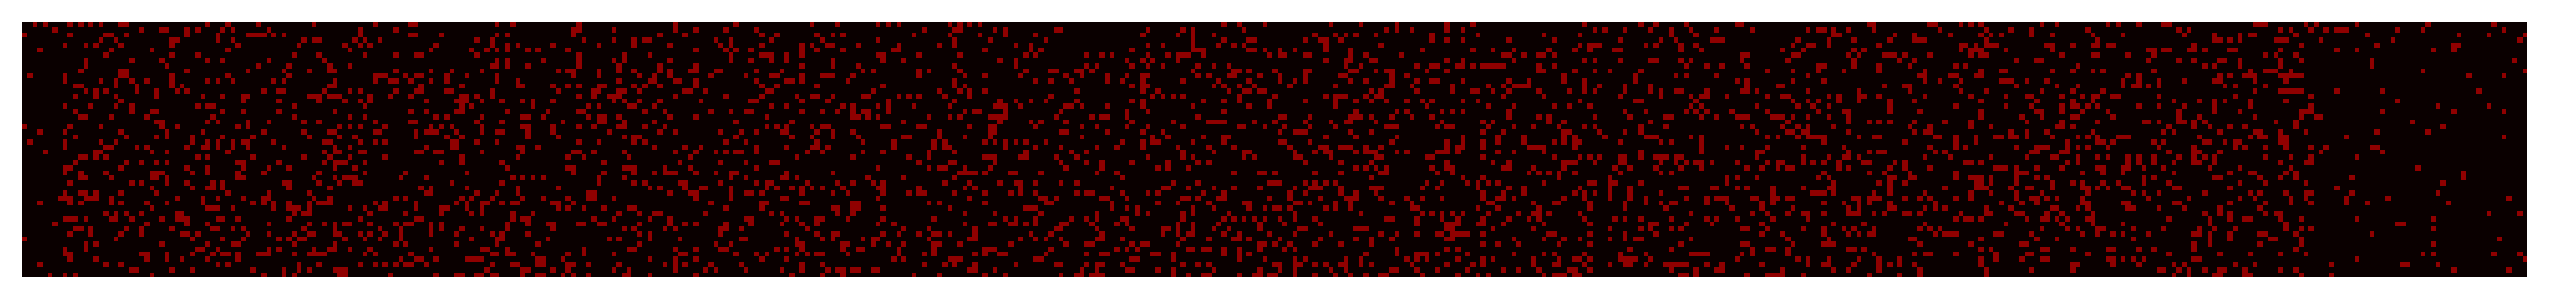
\includegraphics[scale=0.4]{Figs/imagen_fits_1_e.pdf}
    \caption{Imagen resultante luego de ser extraídos los píxeles con carga mayor a $1$ electrón.}
    \label{fig:ImagenFits1e}
\end{figure}
Una vez que se extraen los píxeles de carga mayor a uno, se promedian todas las imágenes resultantes y se obtiene una única imagen que condensa la información de todas las anteriores. En este contexto, promediar las imágenes implica tomar el arreglo matricial con los valores de carga de los píxeles que conforman las imágenes, y realizar la suma convencional de matrices para las más de $900$ imágenes. Finalmente, se divide cada elemento de la matriz suma por la cantidad total de imágenes y se obtiene una imagen donde cada píxel es el promedio de carga de ese píxel para todas las imágenes. De esta forma se puede ver si existen píxeles con mayor o menor tendencia a contener este tipo de eventos.

En la Figura \ref{fig:Eventos1e} se tiene una imagen por cada cuadrante del sensor, promediados en las $\sim 900$ imágenes tomadas, donde los píxeles más brillantes son los que tienen mayor promedio de eventos, es decir, en el total de las imágenes esos píxeles son los que más veces tuvieron un electrón de carga. Esto también puede interpretarse como una imagen de la probabilidad por píxel de que haya un único electrón: Píxeles más brillantes son píxeles más propensos a tener carga.

De la Figura \ref{fig:Eventos1e} pueden destacarse algunas características:
\begin{itemize}
    \item La carga prácticamente nula (en promedio) en las regiones del pre-scan (región izquierda de $7$ columnas de píxeles de extensión) y del over-scan (región derecha de 50 columnas de píxeles de extensión), lo cual es totalmente esperable dado que estos son píxeles con muy baja probabilidad de colectar cargas durante la medición, como fue descripto en la Sección \ref{sec:Mediciones}. Esto se ve para todos los cuadrantes menos el segundo;
    \item El primer cuadrante es en promedio más brillante que el resto, y se observa un ligero gradiente de intensidad entre las filas inferiores y superiores. Esto se repite, pero en menor medida en los demás cuadrantes pero no necesariamente se observa a simple vista. Este efecto se aprecia con mayor claridad en los gráficos de la Figura \ref{fig:GradienteProb};
    \item El segundo cuadrante capta en promedio muy poca carga. Este cuadrante del sensor no funciona correctamente;
    \item En los cuadrantes $3$ y $4$ se pueden ver columnas enteras de píxeles oscurecidas, que captaron muchísima menos carga que podrían deberse a defectos del sensor;
    %\textcolor{red}{es al revés, no están oscurecidas porque capturaron menos carga, sino porque capturaron siempre mas de un electrón y quedaron fuera del conjunto de imágenes con un electrón o vacío a partir de las cuales calculaste la imagen promedio. Es importante decirlo, esas son hot columns y debe ser eliminadas del análisis.}
    \item En todos los cuadrantes (menos el segundo), se observa un único píxel (posición $x = 2$, $y = 0$) donde el promedio de carga es mucho mayor al resto. Además, la primera columna de píxeles luego del pre-scan también tiene tendencia a captar más carga que el resto;
    \item Todos los cuadrantes tienen tendencia a tener \textit{hot píxels} en el interior de la región activa, estos son píxeles aislados que tienden a tener más carga que otros. Además pueden verse líneass verticales de \textit{hot píxeles}, llamadas \textit{hot columns} que se producen debido a que un \textit{hot pixel} está generando carga constantemente mientras estas son desplazadas verticalmente durante la lectura.
\end{itemize}
\begin{figure}[h]
%Para reproducir esta figura hay que ir al directorio /home/igna/Escritorio/Tesis2021/Figs/pys_para_plots y correr Skipper_cuadrantes_plot.py
    \centering
    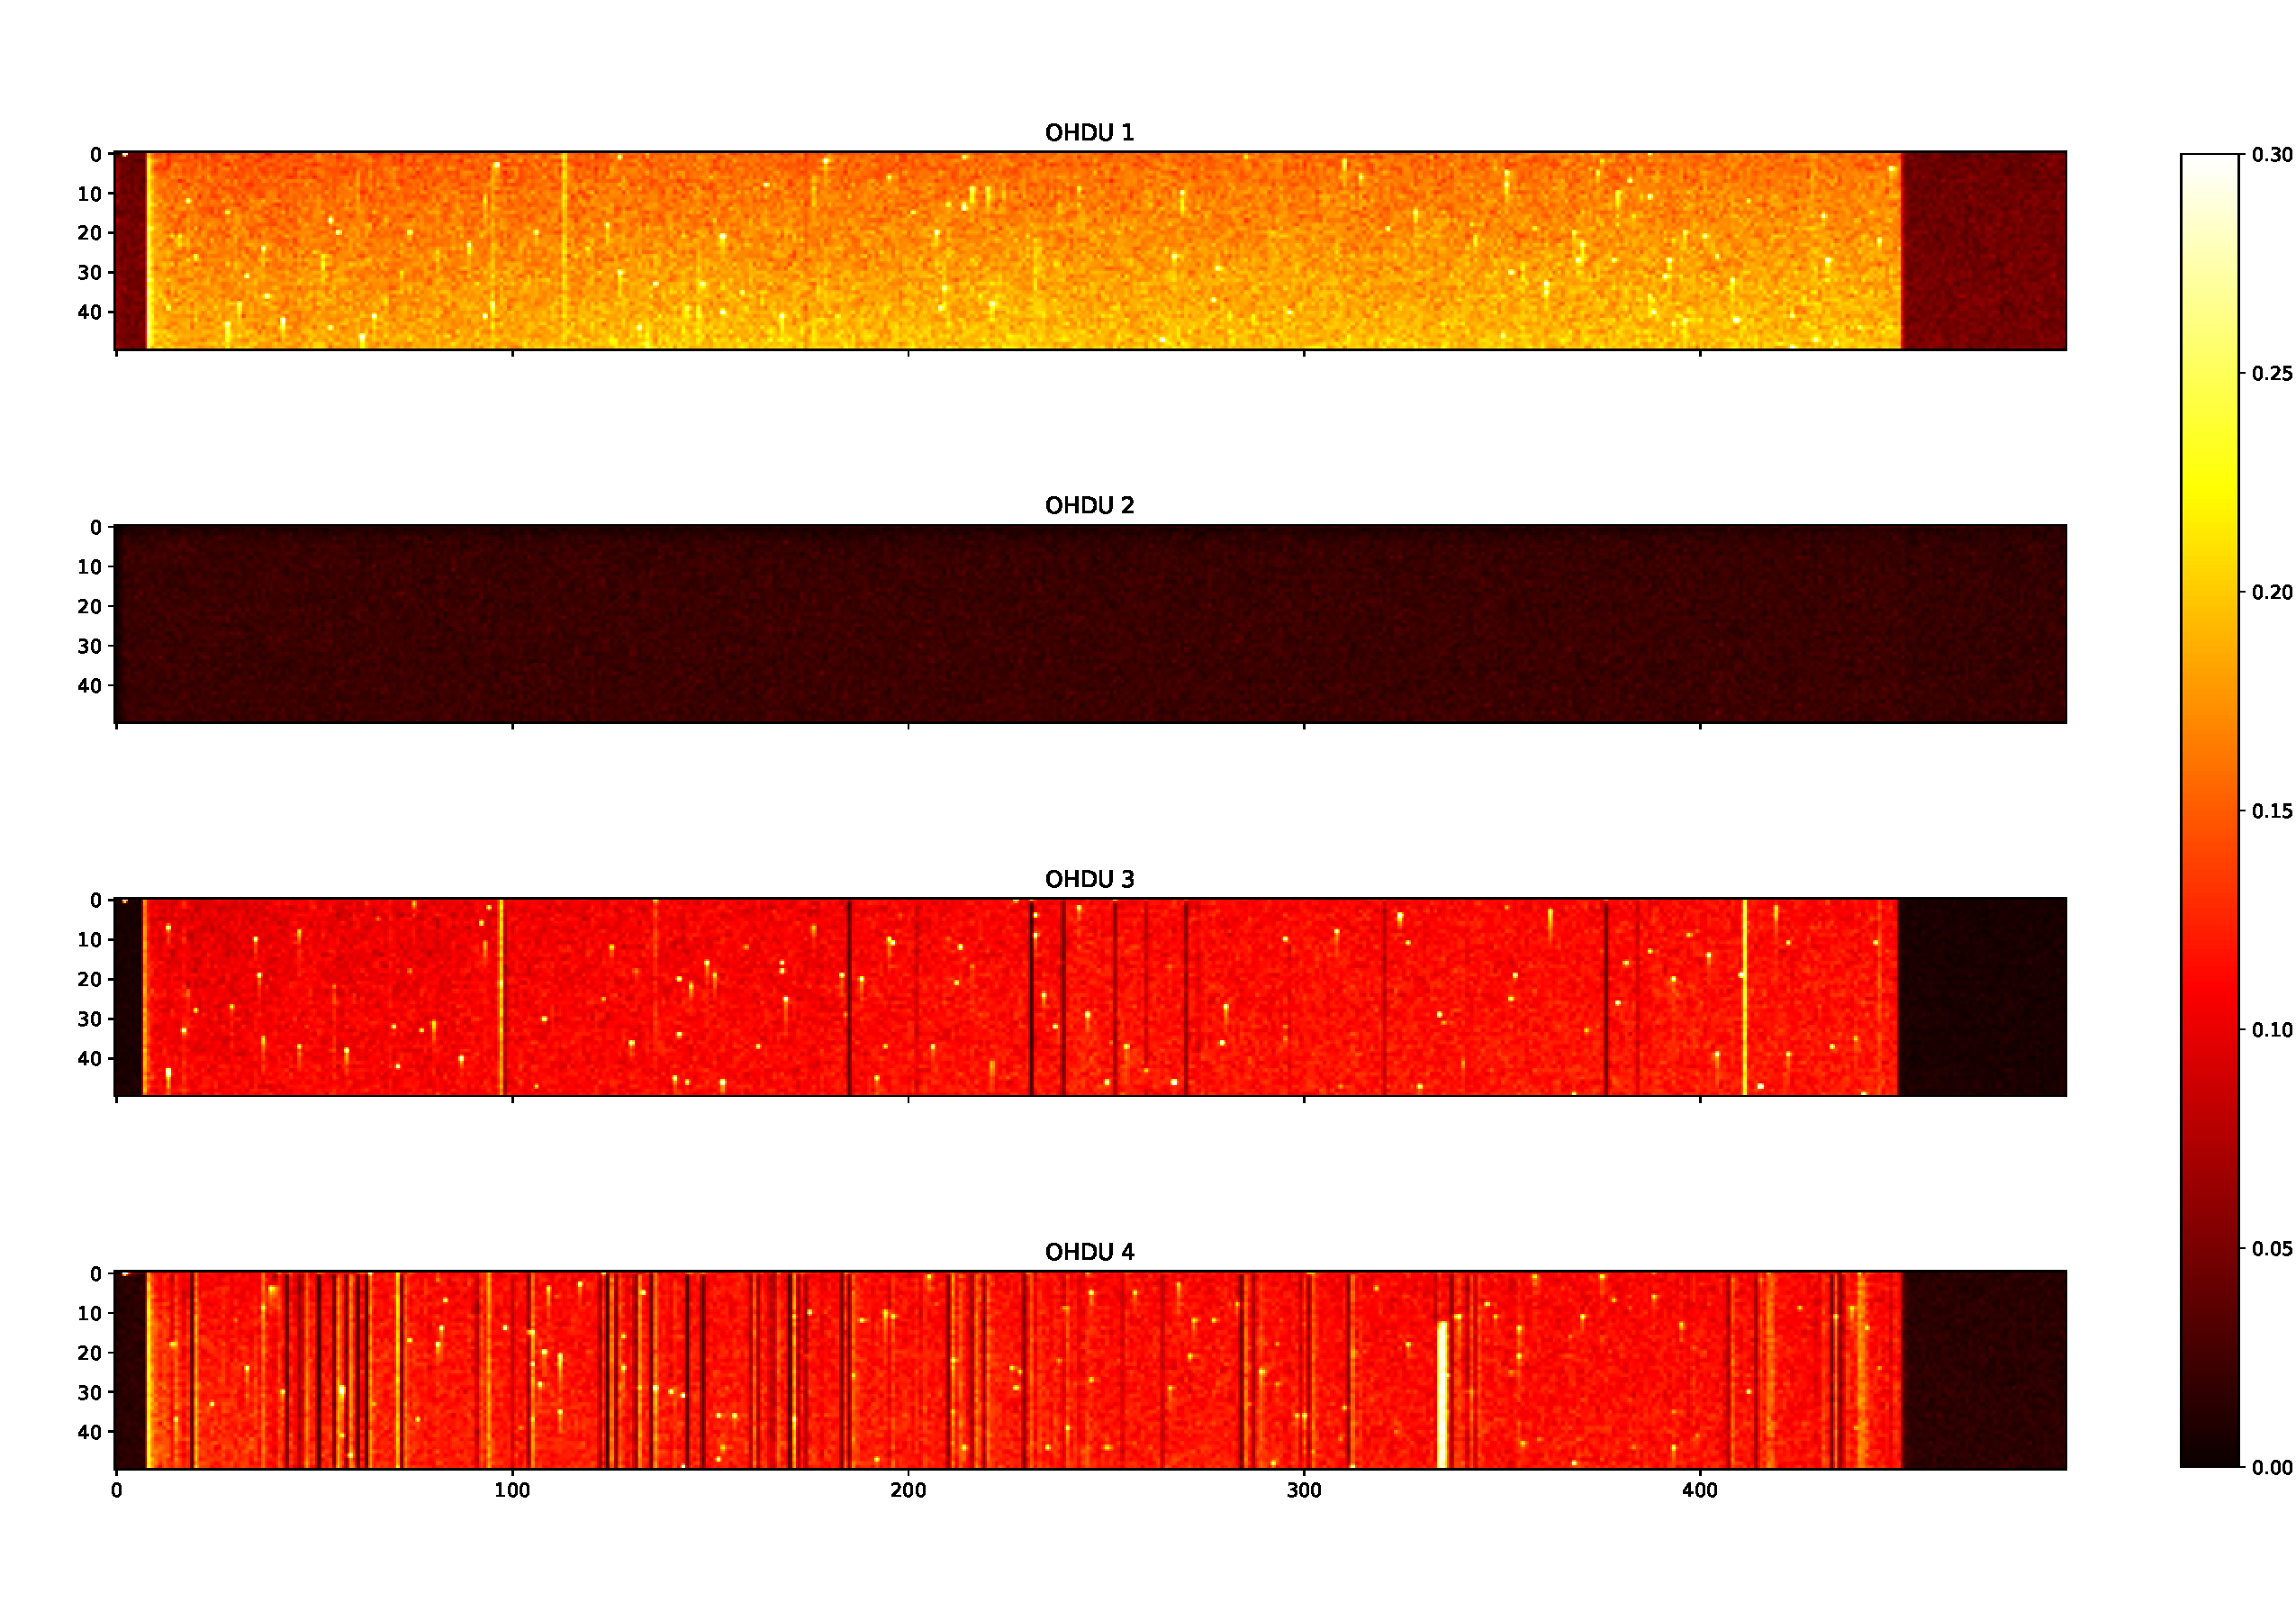
\includegraphics[scale=0.4]{Figs/1ePromedio.pdf}
    \caption{Imágenes promedio para los $4$ cuadrantes del sensor. Puede verse en la escala de la derecha que los valores más altos que se obtienen rondan el $0.3$, lo cual se puede interpretar como un $30\,\%$ de probabilidad de que en ese píxel se encuentre un evento de un electrón. En general se ve que los promedios pueden estar entre $0.1$ y $0.2$ aproximadamente. Es decir, para los cuadrantes funcionales del sensor, cada pixel tiene una probabilidad de tener un único evento que ronda entre el $10\%$ y el $20\%$.}
    \label{fig:Eventos1e}
\end{figure}
Respecto al gradiente de intensidades que se observa entre filas superiores e inferiores de la imagen, implicaría una mayor incidencia de eventos de un electrón, en promedio, en los píxeles de las filas inferiores respecto de las filas superiores. 
%\textcolor{red}{hay que aclarar que significa inferior y superior aca en términos de estar cerca o lejos del sense node. Asi como está pareciera entenderse lo contrario a lo que pasa realmente}
Esto puede observarse en los gráficos de Figura \ref{fig:GradienteProb}, donde se ve el aumento en \textit{la probabilidad} media por fila de que haya un evento de un electrón, a medida que el número de la fila aumenta. El gráfico de arriba a la izquierda corresponde al primer cuadrante del sensor, este es el cuadrante donde más evidente se hace este gradiente, además de ser muy lineal. La probabilidad promedio para la fila $0$ del sensor es $\sim 14.5\,\%$ y crece linealmente hasta $\sim 18\,\%$ para la fila $50$. 
En el gráfico de arriba a la derecha, que corresponde al segundo cuadrante, también se observa un cambio, pero solo entre las primeras 10 filas del sensor, luego la variación de la probabilidad por fila es muy pequeña y parece aproximadamente constante. Además puede verse que los valores son un orden de magnitud menor a los del primer cuadrante. Para los gráficos de abajo a la izquierda y abajo a la derecha, que corresponden a los cuadrantes $3$ y $4$, se observan también variaciones entre las primeras y las últimas filas del sensor y que parecerían tener una tendencia lineal, sin embargo, en comparación a la variación del primer cuadrante, esta es mucho menor. Por esto es difícil verlo a simple vista: la variación para el primer cuadrante es de aproximadamente del $24\,\%$ mientras que la variación de los cuadrantes $3$ y $4$ es aproximadamente del $10\,\%$.

Este gradiente se debe a que, dado que la medición de carga del sensor es secuencial por filas, las filas superiores en la imagen son la filas del sensor que más cerca se encuentran del registro horizontal y del nodo de sensado, con lo cual son las primeras a las que se les mide la carga. Por otro lado, las filas inferiores en la imagen, son las filas del sensor que más lejos se encuentran del registro horizontal y del nodo de sensado, con lo cual permanecen más tiempo expuestas a fuentes de fondo. En la imagen el nodo de sensado se encontraría en la esquina superior izquierda.
\begin{figure}[h]
%Para modificar este plot hay que ir a /home/igna/Escritorio/Tesis2021/Figs/pys_para_plots y correr gradiente_filas_sensor.py Los datos los saca de /home/igna/Escritorio/Tesis2021/Figs/txts_para_plots y del archivo OHDU1/2/3/4_gradiente_filas_sensor.tx
    \centering
    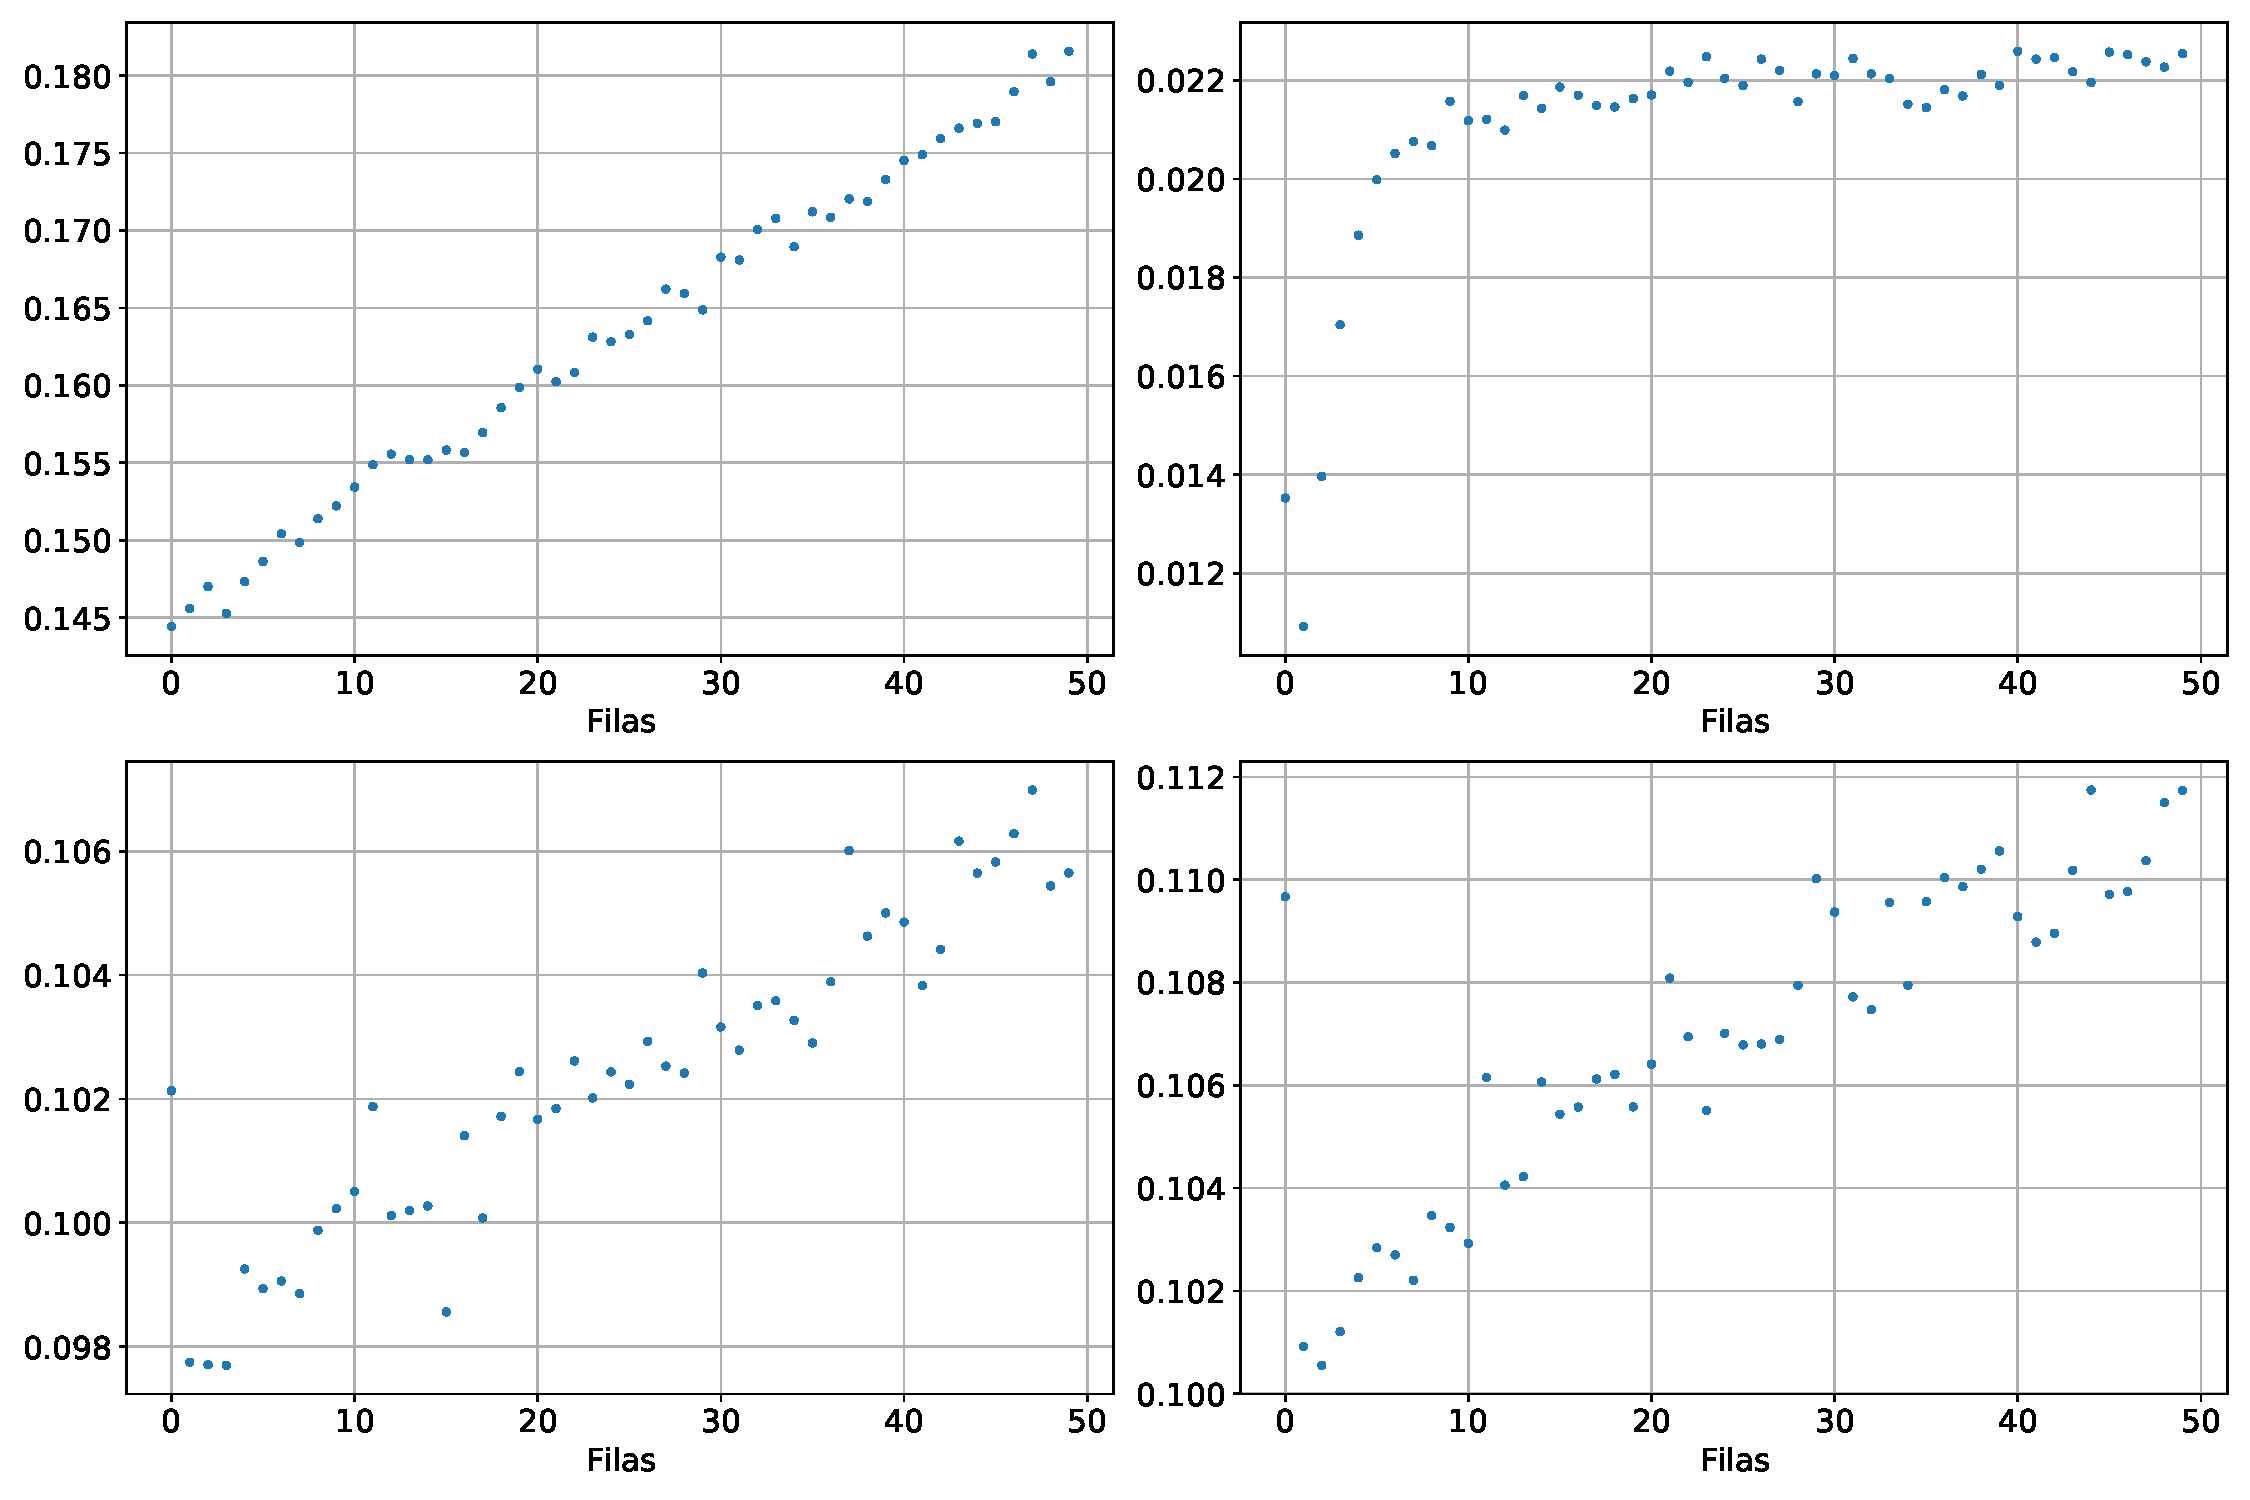
\includegraphics[scale=0.45]{Figs/Gradiente_en_filas_sensor.pdf}
    \caption{Variación de la \textit{probabilidad} promedio por filas del sensor de tener un evento de $1$ electrón, para los diferentes cuadrantes. Se ven aumentos lineales de la probabilidad para los casos de los cuadrantes $1$, $3$ y $4$ y un aumento más pronunciado en relación a los demás para el primer cuadrante.}
    \label{fig:GradienteProb}
\end{figure}

Para los análisis que se realizaron en este trabajo fueron utilizados el primer y tercer cuadrante del sensor, dado que son los cuadrantes que mejor funcionan. El segundo cuadrante es defectuoso y el cuarto cuadrante, si bien funciona, presenta muchas \textit{hot columns} y muchas columnas oscuras, por lo que se decidió omitirlo de los análisis de los histogramas de carga.

%Por otro lado, los análisis que siguen en esta sección se centraron sobre el primer cuadrante dado que es el que mejor funciona de los cuatro.

Teniendo entonces una imagen del promedio de la cantidad de eventos de un electrón por píxel, en la búsqueda por caracterizar el fondo del sensor, lo que se hizo posteriormente fue promediar todos los elementos de esta, de forma de obtener un promedio total y poder interpretarlo como una \textit{probabilidad} general de que en un píxel haya un evento de un electrón. Entonces, para el primer cuadrante y considerando solo la región activa del sensor, se obtuvo una probabilidad $\bar{p} = 0.1802 \pm 0.0213$, es decir, que con esta primera manera de caracterizar el fondo, hay aproximadamente un $18\,\%$ de probabilidad de que un dado píxel de la región activa del sensor tenga un electrón.

Sin embargo, esta es una forma muy rudimentaria para intentar caracterizar el fondo, además de que no es del todo correcta. Con este camino se asume que todos los eventos de un electrón son fondo, lo cual no es correcto, de forma que la probabilidad de tener un evento de un electrón en un dado píxel, calculada de esta manera, está sobrestimada. 

Un camino más sofisticado para estimar el fondo en el sensor es explotando el hecho de que los eventos medidos en él siguen una distribución poissoniana: si se supone que todo píxel tiene igual probabilidad de tener una carga debido a fondo, que dicha probabilidad es pequeña para mediciones de corto tiempo y que el número de píxeles es muy grande ($22150$ píxeles por cuadrante), entonces es esperable que la distribución que modela estos eventos sea una poissoniana. De esta forma, si se pudiera calcular la esperanza $\mu$ de la distribución, podría saberse la probabilidad de que en un determinado píxel se encuentre un evento de un electrón o, en general, la cantidad de electrones que se desee.

%%%%%%%%%%%%%%%%%%%%%%%%%%%%%%%%%%%%%%%%%%%%%%%%%%%%%%%%%%%%%%%%%%
\section{Estimación del fondo}
\noindent Si se considera una distribución poissoniana para la variable aleatoria \textit{número de electrones de fondo por píxel}, dada por:
\begin{equation*}
    P(k|\mu) = \frac{\mu^{k}\,e^{-\mu}}{k!},
\end{equation*}
se puede tomar el caso $p = P(k = 1 | \mu) = 0.1802 \pm 0.0213$, que es la probabilidad que se obtuvo previamente para el primer cuadrante. A partir de esta se puede despejar numéricamente el valor $\mu$ que satisface la expresión anterior y resulta ser
%De forma itera partiva \textcolor{red}{qué significa de forma iterativa?}puede hallarse el valor de $\mu$ que satisface la expresión anterior y resulta ser
\begin{equation*}
    \bar{\mu} = 0.2258 \pm 0.0271
    % PARA VER EL CALCULO DE ESTO:Analisis_imagenes_probabilidades.ipynb
    % PRIMER MÉTODO: PROMEDIO SIMPLE
\end{equation*}
Si bien esta forma de cuantificar el fondo es un poco más general, dado que ahora pueden contemplarse casos más raros, como que un píxel tenga más de una carga, este método sigue teniendo el problema de la sobrestimación de la probabilidad por píxel, al seguir asumiendo que todo píxel con un electrón proviene del fondo.

Siguiendo sobre el mismo camino, todavía bajo la hipótesis de que todo evento de un electrón es debido a fondo, pero evitando el cálculo de los promedios, hay una forma de calcular la esperanza de la distribución y es notando lo siguiente: si se toman las probabilidades de que haya una sola carga y ninguna carga por píxel, es decir, se toman
\begin{equation*}
    p_{0} \equiv P(k = 0 | \mu),
    \quad
    \quad
    p_{1} \equiv P(k = 1 | \mu)
\end{equation*}
y se mira la relación entre ambas, se tiene
\begin{equation*}
    \frac{p_{1}}{p_{0}} = \frac{\mu\,e^{-\mu}}{e^{-\mu}} = \mu
\end{equation*}
y se observa que puede hallarse directamente el valor de la esperanza de la distribución. Entonces, tomando la región activa de una imagen completa, con todos sus eventos, como la de la Figura \ref{fig:ImagenFitsOriginal}, contando la cantidad de píxeles vacíos, la cantidad de píxeles con un electrón y calculando la relación entre ambas, para todas las imágenes, se puede obtener directamente una estimación para el parámetro $\mu$ de la distribución. De esto se obtuvo que el valor es:
\begin{equation*}
    \bar{\mu} = 0.2311 \pm 0.0001
\end{equation*}
Los resultados de ambos métodos difieren en menos del $5\,\%$ y se solapan sus errores. 
%Si bien esta segunda forma para calcular la esperanza $\mu$ parece un poco más elegante y correcta, el problema sigue estando en los datos que se utilizan para calcularla. 
Sin embargo, el valor seguirá estando sobrestimando respecto del valor real, en tanto se siga considerando a todo píxel con un único electrón como fondo.

No hay que perder de vista que el objetivo de calcular la esperanza de la distribución es poder utilizarla para estimar cuánta carga extra hay sobre los clusters debida a fondo y cuánta carga no espuria fue removida debido al umbral aplicado. 
%
Conociendo la esperanza de la distribución de eventos de fondo y la cantidad de píxeles que ocupa un cluster, puede calcularse la cantidad esperada de carga extra que se halla en cada cluster. Teniendo estos valores, puede corregirse el sesgo introducido en el valor de la carga de cada cluster debido al corte aplicado y con eso hacer una mejor determinación del factor de Fano y la energía de creación electrón-hueco.
%
% Pero también, para poder generar una corrección completa para el conteo de cargas por cluster, hay que tener en cuenta las posibles formas en las que un cluster podría tener más o menos carga:
% \begin{itemize}
%     \item Que sobre la superficie de los clusters hayan eventos de más debido a fondo;
%     \item Dado que en este análisis se está aplicando un umbral que elimina eventos de un electrón y podría suceder entonces que a un cluster se le quiten eventos reales que se encuentran en sus bordes.
% \end{itemize}
% \textcolor{red}{-----------------------------------------------------------------}
% \textcolor{red}{Este itemizado de casos llega tarde, hay que hacerlo antes y completo para que el lector pueda seguir el texto.}
% \textcolor{red}{-----------------------------------------------------------------}
Con lo cual no solo es necesario corregir la carga por exceso en los clusters, sino también por defecto. Por ello, la esperanza que se obtuvo de calcular la relación entre eventos de un electrón y píxeles vacíos contiene tanto información de eventos espurios como información de eventos genuinos. Pero lo que se persigue es poder identificar los eventos espurios y los genuinos por separado. En ese sentido puede decirse que 
\begin{equation*}
    \mu_{T} = \mu_{bkg} + \mu_{g}
\end{equation*}
donde $\mu_{bkg}$ es la esperanza de la distribución de la variable aleatoria \textit{cantidad de eventos espurios por píxel}, mientras que $\mu_{g}$ es la esperanza de la variable aleatoria \textit{cantidad de eventos genuinos por píxel}. Hay que lograr separar ambos efectos para poder aplicar las correcciones correctamente. 
Queda claro que hasta el momento solo se calculó $\mu_{T}$, sin poder discriminar ambas contribuciones. La forma en la que se llevó a cabo la separación entre ellas se detalla a continuación.

%%%%%%%%%%%%%%%%%%%%%%%%%%%%%%%%%%%%%%%%%%%%%%%%%%%%%%%%%%%%%%%%%%
\subsection{Cálculo de las contribuciones de carga}
\noindent Hasta el momento, ambos métodos utilizados para calcular $\mu_{T}$ consistían en analizar los eventos de un electrón en toda el área activa del sensor. Sin embargo, esto traía aparejada una sobre estimación en los cálculos dado que se asumió que todo evento de un electrón era fondo, lo cual no es cierto. Por otro lado, considerando que la distribución de eventos por píxel tiene tanto contribuciones de fondo como genuinas, es necesario poder separar ambas contribuciones y no existe forma de hacerlo al estudiar el área activa del sensor sin tener en cuenta la posición de los clusters.

Para poder separar ambas contribuciones al calcular el $\mu_{T}$, se puede restringir el análisis al entorno cercano de los clusters, donde ahora por clusters se entiende todo conjunto de píxeles donde cada uno tenga como mínimo dos electrones de carga (eventualmente podría ser un único píxel). Es decir, se toma una imagen que tiene eventos de dos o más electrones, y se remueven los píxeles con un sólo electrón. 
En la imagen de la Figura \ref{fig:ImagenFits2omasElectrones} se muestra como luce una imagen luego de aplicar este corte.
\begin{figure}[h]
%Para modificar este plot hay que ir a /home/igna/Escritorio/Tesis2021/Figs/pys_para_plots y correr imagen_fit_2_o_mas_e.py
    \centering
    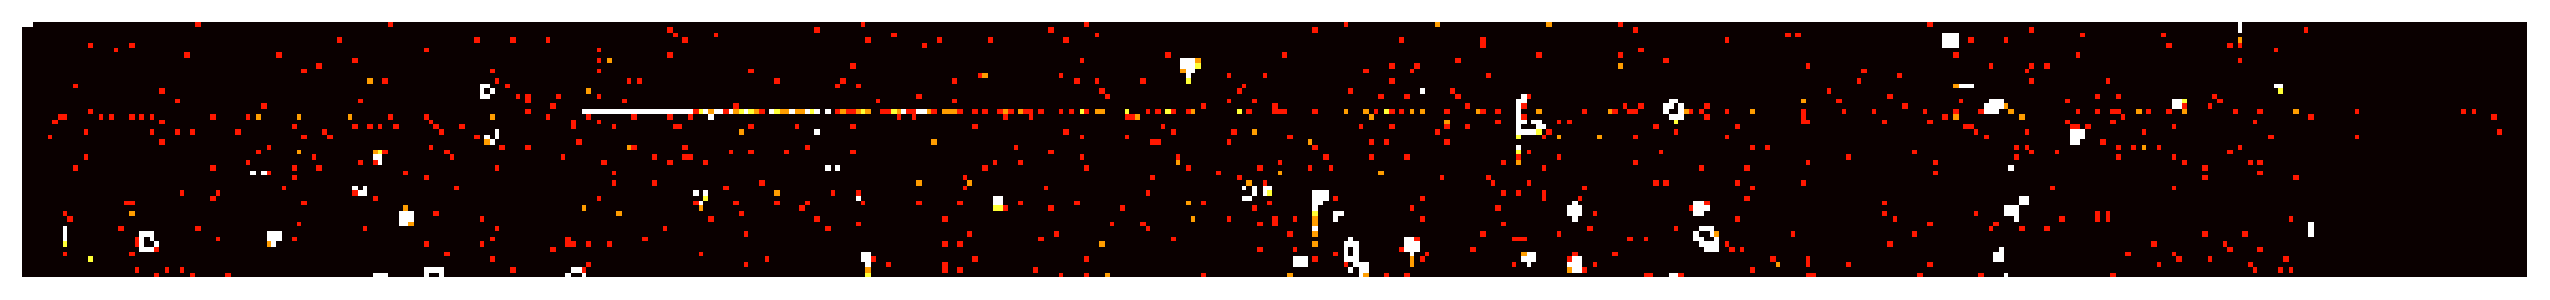
\includegraphics[scale=0.4]{Figs/imagen_fits_2_o_mas.pdf}
    \caption{Imagen de ejemplo en la que se han eliminado todos los eventos de un electrón.}
    \label{fig:ImagenFits2omasElectrones}
\end{figure}
En el entorno cercano de los clusters, más precisamente, en los píxeles inmediatamente contiguos a los píxeles con carga, a partir de ahora  \textit{primer borde}, es la región donde se puede decir con seguridad que coexisten ambas contribuciones: fondo y eventos genuinos. En cambio, la región formada por los píxeles que se encuentran separados por un píxel entre ellos y los eventos, a partir de ahora \textit{segundo borde}, es la región donde la probabilidad de que haya eventos de un electrón que sean genuinos y que por difusión terminaron alejados de su cluster es tan baja que puede considerarse nula. 
Con lo cual, en esta región y toda región más lejana a los clusters puede considerarse que los eventos de un electrón que se encuentren solo pueden deberse a fondo.

Sabiendo que existe una región donde se encuentran ambas contribuciones juntas y otra región donde solo se puede encontrar la contribución de fondo se pueden calcular y obtener ambas contribuciones por separado.

El método utilizado consistió en tomar el primer borde de los clusters para calcular allí el valor de $\mu_{T}$. El procedimiento se basó en formar una máscara del primer borde de los clusters. Para eso se tomaron todos los eventos de dos o más electrones y se los expandió un píxel en todas las direcciones para formar la primera etapa de la máscara. Luego, se vacío el interior de esta dejando solo sus contornos, que coinciden con los píxeles contiguos a los bordes de los clusters. Luego, superponiendo la máscara sobre la imagen original (ahora con todos los eventos), se cuentan los píxeles con eventos de un electrón y los píxeles vacíos cayeron sobre la máscara. 
\begin{figure}[H]
%Para modificar este plot hay que ir a /home/igna/Escritorio/Tesis2021/Figs/pys_para_plots y correr imagen_bordes2.py
    \centering
    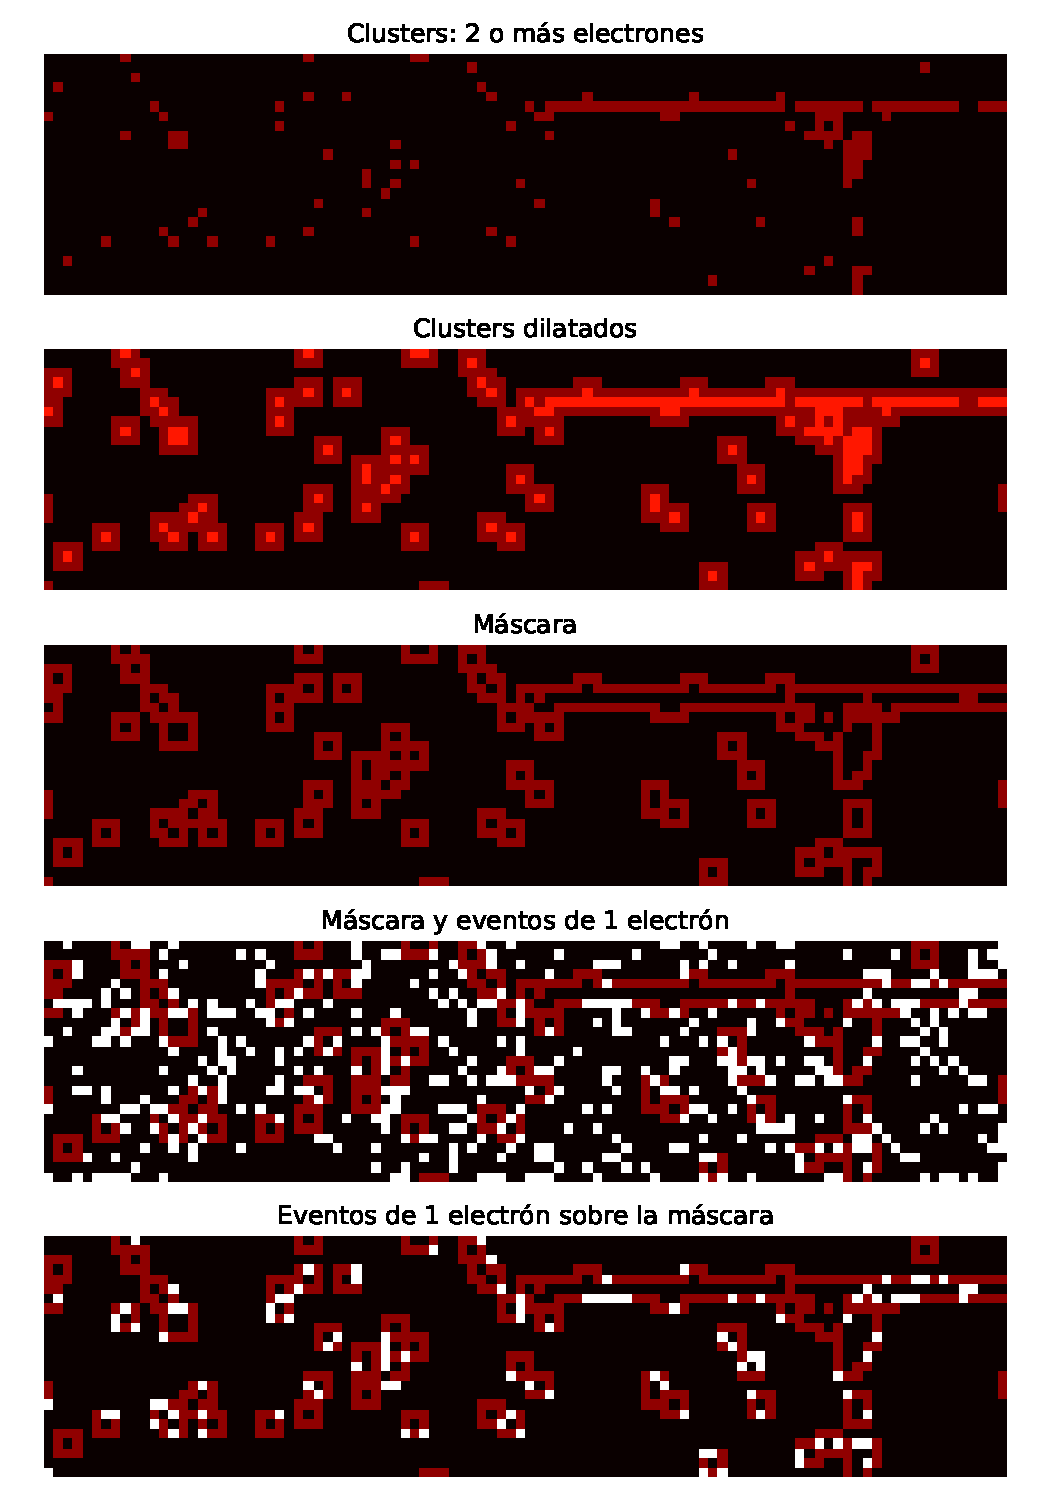
\includegraphics[scale=0.65]{Figs/analisis_bordes.pdf}
    \caption{Diferentes partes del proceso de análisis de los bordes de los clusters para una imagen de ejemplo. En cada figura se ve una porción de $25 \times 100$ píxeles de área. En la primera imagen (de arriba a abajo) se tienen los clusters de dos o más electrones. En la segunda imagen se representa la dilatación de los clusters aumentando en un píxel en todas las direcciones. En la tercera imagen se ve la diferencia entre las dos primeras imágenes y se la define como la máscara a utilizar. En la cuarta se ve la máscara y superpuestos todos los eventos de un electrón de esa porción del sensor. Finalmente, en la quinta se ven solo los eventos de un electrón que cayeron encima de los píxeles de máscara. Son estos eventos los que son se cuentan en todas las imágenes, junto con los píxeles vacíos de la máscara para calcular el $\mu_{T}$.}
    \label{fig:AnalisisBordes}
\end{figure}
Nuevamente, calculando la relación entre eventos de un electrón y píxeles vacíos, se obtiene para el primer cuadrante $\bar{\mu}_{T} = 0.2049 \pm 0.0002$, dado que en el primer borde se encuentran las dos contribuciones. En la Figura \ref{fig:AnalisisBordes} puede verse gráficamente cada uno de los pasos que se llevó a cabo para generar la máscara y contabilizar los eventos de un electrón que se solapan con ella.

Conociendo el valor de $\mu_{T}$, resta obtener la contribución del fondo que da origen a $\mu_{bkg}$. En primer lugar se ensayó utilizar la región conformada por el segundo borde y los píxeles aún más lejanos para calcular el $\mu_{bkg}$, es decir, toda la región restante del sensor donde hay eventos espurios. Para esto, utilizando la máscara previamente obtenida, en vez de observar los eventos de un electrón de la imagen original que solapan con ella, se cuentan los eventos de un electrón y los vacíos que están fuera de ella. De calcular la relación entre ambos, como se hizo previamente, se obtiene que el valor para el valor medio de la contribución del fondo es $\bar{\mu}_{bkg} = 0.1621 \pm 0.0001$. 

Sin embargo, esta forma de calcular el fondo puede mejorarse un poco más. El objetivo del cálculo de estos valores medios es poder utilizarlos para corregir la carga medida en los clusters, debido al fondo y al umbral utilizado. Es por eso que los valores de las contribuciones que se están buscando deben ser las más representativas para los sesgos de estos eventos. Utilizar eventos de un electrón que se encuentran lejos de los eventos de interés para calcular estas correcciones no sería del todo correcto. Con lo cual, para calcular el valor de $\mu_{bkg}$ más representativo a los clusters, se optó por mirar únicamente el segundo borde y no todo el resto del sensor.

El procedimiento es el mismo que para el primer borde, pero ahora expandiendo los clusters en dos píxeles en todas las direcciones, y quedándose únicamente con el segundo borde, donde no hay píxeles con carga genuina y donde se tienen los eventos de fondo más representativos para los clusters. Este proceso puede verse en la imagen \ref{fig:AnalisisBordesx2}. Nuevamente, de la relación entre los eventos de un electrón y los píxeles vacíos que se solapan con la máscara, se obtiene para el primer cuadrante $\bar{\mu}_{bkg} = 0.1902 \pm 0.002$. Finalmente, teniendo el valor de $\mu_{T}$ y el valor de $\mu_{bkg}$ queda completamente determinado el valor de $\mu_{g}$.
\begin{figure}[H]
%Para modificar este plot hay que ir a /home/igna/Escritorio/Tesis2021/Figs/pys_para_plots y correr imagen_bordesx2.py
    \centering
    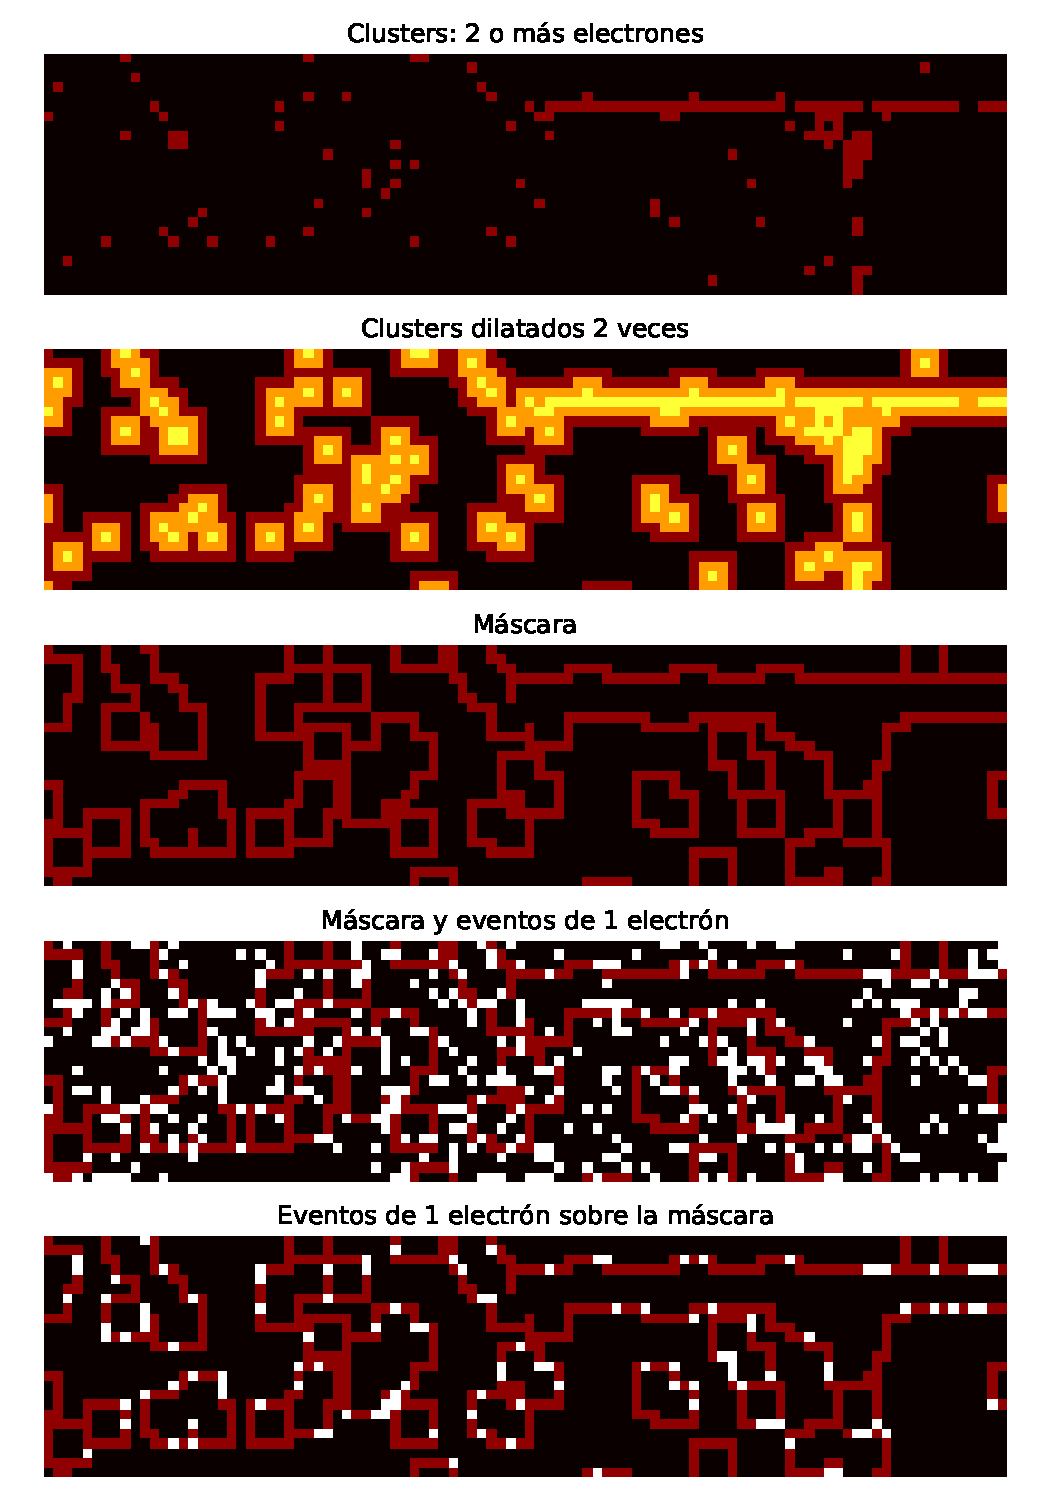
\includegraphics[scale=0.65]{Figs/analisis_bordesx2.pdf}
    \caption{Análoga a la Figura \ref{fig:AnalisisBordes}, pero para el caso de $2$ dilataciones, de forma de generar una máscara en el segundo borde. Los pasos son los mismos antes descriptos. De este proceso se halla la esperanza $\mu_{bkg}$.}
    \label{fig:AnalisisBordesx2}
\end{figure}
De realizar estos análisis se obtuvieron los valores para las esperanzas de ambas contribuciones, calculadas sobre el conjunto de más de $900$ imágenes provenientes de mediciones de los rayos $X$ del flúor y para el primer cuadrante del sensor, que resultaron ser:
\begin{equation*}
    \bar{\mu}_{T} = 0.2040 \pm 0.0002
\end{equation*}
y el valor de la esperanza para los eventos espurios resultó 
\begin{equation*}
    \bar{\mu}_{bkg} = 0.1961 \pm 0.0002
\end{equation*}
con lo cual, la esperanza para los eventos genuinos es 
\begin{equation*}
    \bar{\mu}_{g} = 0.0079 \pm 0.0003   
\end{equation*}
El mismo análisis puede repetirse para los demás cuadrantes. En este caso se decidió repetirlo para el tercer cuadrante que fue el otro cuadrante que se utilizó en los resultados de este trabajo, obteniéndose:
\begin{equation*}
    \bar{\mu}_{T} = 0.1357 \pm 0.0003
\end{equation*}
\begin{equation*}
    \bar{\mu}_{bkg} = 0.1186 \pm 0.0002
\end{equation*}
\begin{equation*}
    \bar{\mu}_{g} = 0.0172 \pm 0.0004   
\end{equation*}

%%%%%%%%%%%%%%%%%%%%%%%%%%%%%%%%%%%%%%%%%%%%%%%%%%%%%%%%%%%%%%%%%%
\subsection{Corrección al sesgo en el conteo de carga}
\noindent El punto del análisis anterior era generar las herramientas para corregir el conteo de carga que hace el programa de reconstrucción de eventos luego de aplicar el umbral que elimina todos los eventos menores a dos electrones y dado que estos pueden también tener eventos extra debido a fondo.

Esta corrección se llevó a cabo modificando el código del programa que es usado por \textit{ROOT} para calcular el factor de Fano, la energía de creación electrón-hueco, y otras variables por medio del ajuste no bineado de los espectros de carga. Los espectros son reconstruidos utilizando la información de los clusters que está contenida en el archivo \verb|.root| generado por \verb|skExtract.exe| al procesar las imágenes, como se describió en la Sección \ref{sec:ProcesadoDatos}. Al contar la carga de estos clusters y conociendo el área de los mismos (cantidad de píxeles que los conforman), se agrega y se quita carga en función de los valores hallados en la sección anterior.

%Dado que la cantidad de carga por píxel sigue una distribución poissoniana, de esperanza $\mu$, para cada tipo evento (espurio, genuino o total) se tiene una esperanza. 
Para calcular la cantidad de carga que se espera que tenga un cluster de $N$ píxeles, se puede hacer uso de las propiedades de la esperanza. Sea $Y = \sum\limits_{i = 1}^{N} X_{i}$, donde $X_{i}$ son distintas realizaciones de la variable aleatoria con distribución poissoniana y $N$ es el número de píxeles del cluster, entonces la esperanza de la nueva variable aleatoria $Y$ se calcula como
\begin{equation*}
     E(Y) = 
     E
     \left(
         \sum\limits_{i=1}^{N} X_{i}
     \right)
     = \sum\limits_{i=1}^{N}E(X_{i})
     = \sum\limits_{i=1}^{N}\mu_{i}
\end{equation*}
pero como $X_{i}$ son distintas realizaciones de la misma variable aleatoria, entonces tienen todas la misma esperanza, es decir $\mu_{i} = \mu\ \forall\ i$, con lo cual
\begin{equation*}
    E(Y) = N\mu
\end{equation*}
es por esto que la cantidad de carga esperada para un cluster viene dada por el producto entre la esperanza de la distribución y la cantidad de píxeles del cluster. De esta forma, sabiendo que la esperanza se puede escribir como $\mu_{T} = \mu_{bgk} + \mu_{g}$, las correcciones se pueden realizar aplicando esta misma receta a los valores de carga por cluster: se espera que la carga genuina removida por el umbral sea $N\mu_{g}$ y que la carga de fondo en su interior sea $N\mu_{bkg}$. Este proceso puede realizarse dado que, para los tamaños de los eventos con los que se trabaja existe una relación casi $1$-$1$ entre su área y la cantidad de píxeles en sus bordes, como se observa en la Figura \ref{fig:relacion_area_perimetro}.
\begin{figure}[h]
%Para modificar este plot hay que ir a /home/igna/Escritorio/Tesis2021/Figs/pys_para_plots y correr imagen_bordesx2.py
    \centering
    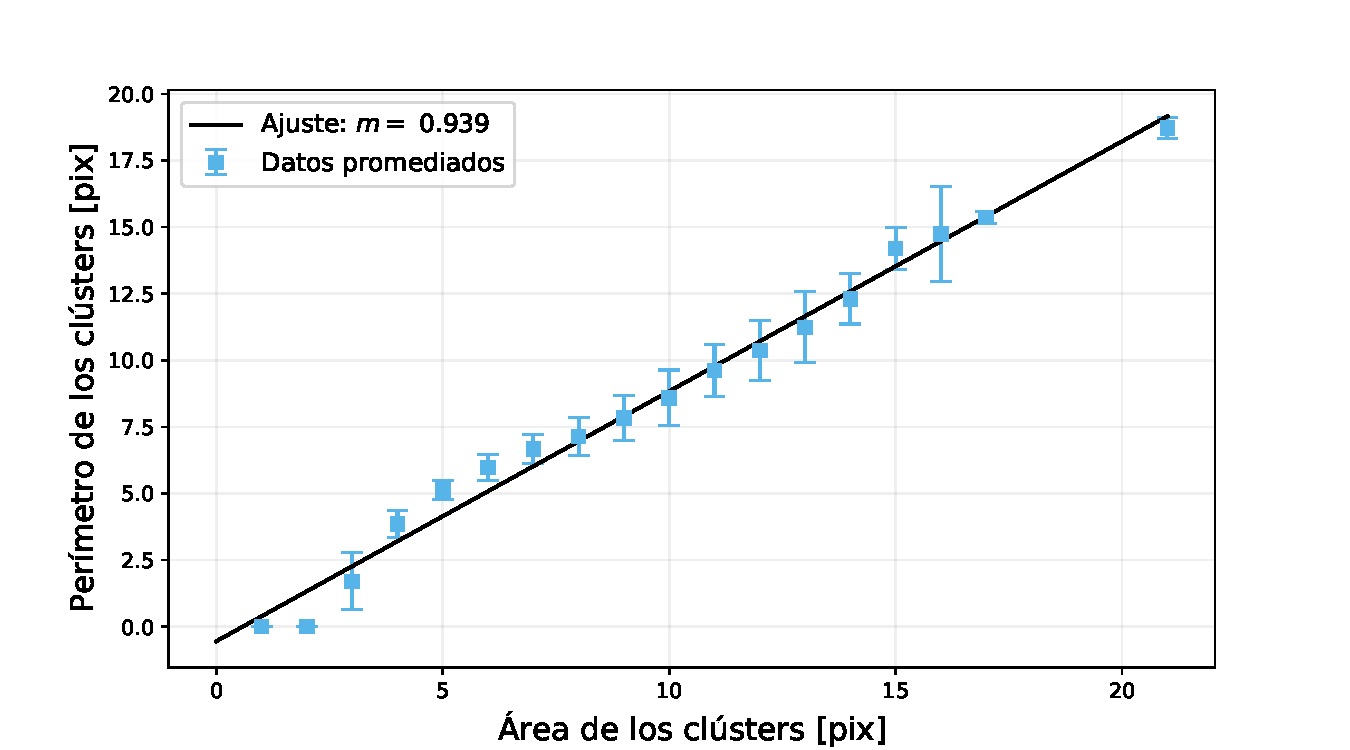
\includegraphics[scale=0.5]{Figs/clusters_perimetro_vs_area.pdf}
    \caption{Perímetro promedio de los clusters, en función de área o cantidad de píxeles. Se ajustan los datos con una recta cuya pendiente resultó $m = 0.938 \pm 0.026$, lo cual permite usar áreas como estimador de las superficies.}
    \label{fig:relacion_area_perimetro}
\end{figure}
Cabe destacar que la aplicación de las correcciones se realiza sobre los datos a los cuales ya se les ha aplicado el corte en el umbral para elmininar eventos de un electrón, de forma que el fondo presente en los bordes de los clusters ya ha sido removido, al igual que los eventos genuinos que pudiera haber en ellos. Si $n_{e}$ es la cantidad de carga medida en un dado cluster, la corrección de este valor de carga será $n_{c}$ y viene dada por
\begin{equation*}
    n_{c} = n_{e} + N(\mu_{g} - \mu_{bkg})
\end{equation*}
es decir, se agrega la cantidad de carga que se estima se pierde en los bordes por aplicar el umbral \verb|EPIX=1.5| y se quita la carga estimada de fondo en el interior de los clusters. En la práctica este procedimiento es simplemente agregar una línea en el código, justo después de la medición de carga de un cluster, donde se actualiza el valor de carga con la expresión anterior.

El método descripto se utilizará para corregir el sesgo introducido al cambiar \verb|EPIX| y el preexistente por el fondo. Los resultados finales se presentan en el Capítulo \ref{chap:Resultados}.
    
    \chapter{Resultados}
Sección pendiente porque faltan los resultados. Etiam accumsan non nulla porta lacinia. Curabitur auctor neque ac nulla efficitur fringilla. Phasellus euismod ante id elit faucibus, condimentum condimentum dui viverra. Etiam in nunc semper, hendrerit leo at, bibendum orci. Fusce feugiat at velit ut blandit. Maecenas consectetur condimentum elit, vel venenatis diam pharetra ut. Curabitur vel sapien vitae purus placerat rhoncus nec sit amet dui. Cras vehicula dictum dignissim. Donec placerat mauris in nisl feugiat dictum. Nam dui tortor, rhoncus sed metus at, finibus bibendum libero. Sed nec pharetra lacus, ac pretium mauris. Proin a augue commodo, imperdiet ex vitae, aliquet orci. In condimentum elementum metus in bibendum. Sed tempus augue sit amet tellus posuere posuere. In et suscipit eros, nec interdum nulla. Vestibulum blandit, lorem et viverra dapibus, diam lectus ultricies augue, ut gravida justo quam sed ligula.


    
	\chapter{Conclusiones}
faltan las conclusiones Phasellus at pharetra nisl. Morbi eu mi dolor. Maecenas sagittis, eros quis vulputate egestas, velit tellus rutrum metus, a condimentum risus nunc et lorem. Pellentesque ornare placerat accumsan. Donec pulvinar lorem augue, nec pharetra eros condimentum sed. Phasellus nec lacinia sem, at tincidunt lectus. Maecenas non blandit orci. Curabitur ullamcorper, elit id iaculis rutrum, enim leo auctor purus, a porttitor elit leo et libero. Nam pellentesque, orci vitae posuere lacinia, leo turpis iaculis lorem, sit amet fermentum nunc turpis et tortor. Maecenas mollis risus enim, at dignissim magna rhoncus et.


	
	\appendix
\chapter{Implementación del código de la simulación \label{app:Implementación}}
%\section{Implementación del código de la simulación}
\noindent La implementación de los códigos que ejecutan la simulación Monte Carlo se realizó con los lenguajes C y Python. Con C se realiza todo el trabajo de alto costo computacional, mientras que Python cumple un rol de interfaz de entrada para los parámetros de la simulación, de procesamiento de los datos obtenidos de ella y de visualización de resultados por medio de gráficos.

A grandes rasgos, en el código en C están implementadas las funciones que hacen los cálculos antes mencionados: el cálculo de la probabilidad de ionización $P_{eh}$ a partir de la expresión \eqref{ec:ProbabilidadIonizacion}, el cálculo del parámetro $\alpha = \alpha(E_{R})$ para la distribución Beta, a partir de la cual se genera una realización de la variable aleatoria de la que se puede despejar la energía transferida a un par electrón-hueco por ionización. Finalmente, por recursión, se simulan los procesos de ionización en cascada y se cuenta la cantidad final de electrones ionizados.

La parte escrita en Python se encarga de ejecutar el programa en C las veces que sean necesarias y con los parámetros iniciales de interés para obtener el resultado buscado.

Más en detalle, el programa en C consta de un total de $6$ funciones, las cuales se listan a continuación con una breve descripción de su funcionamiento
\begin{enumerate}[label=\arabic*., listparindent=1.5em]
    \item \verb|Random()|: Esta función genera realizaciones \verb|p_rand| de una variable aleatoria de distribución uniforme, entre $0$ y $1$. Se usa para generar una probabilidad de comparación en el Monte Carlo.
    \item \verb|Peh(E_r, A)|: Esta se encarga de realizar el cómputo de la probabilidad de ionización, según la ecuación \eqref{ec:ProbabilidadIonizacion}, a partir de la energía $E_{R}$, que es un argumento inicial en el programa y es ingresado desde Python. Esta probabilidad, \verb|p_eh|, se compara con \verb|p_rand| en el algoritmo de aceptación del Monte Carlo.
    \item \verb|alpha(E_r)|: Calcula el valor del parámetro $\alpha$ en base al valor del parámetro \verb|E_r|. Si bien el parámetro \verb|E_r| es un parámetro inicial que, por ejemplo, para el flúor es $677\,\si{eV}$, a medida que evoluciona el sistema, la energía se va consumiendo en ionizacionar y este parámetro cambia. Con cada actualización se calcula nuevamente el valor de $\alpha$ para la distribución Beta. El valor del parámetro se calcula entonces como
    \begin{equation*}
        \alpha =
        \left\{ \begin{array}{lcc}
             0.1 & \mbox{si} & E_{r} < E_{g}\\
             1 & \mbox{si} & E_{g} < E_{r} < 4.2\,\si{eV}\\
             0.02E_{r} + 0.95 & & \mbox{en otro caso.}
             \end{array}
        \right.
    \end{equation*}
    \item \verb|evolucionar(E_r, A, rand_beta)|: Genera la evolución del sistema mediante el algoritmo de aceptación del Monte Carlo, haciendo uso de las funciones anteriores. Implementa un bucle \verb|while|, cuya condición es que se repita el proceso mientras que la energía \verb|E_r| sea mayor que la energía del gap del silicio \verb|E_g|. Dentro del bucle se calcula la probabilidad \verb|p_eh| de ionización, el parámetro $\alpha$, que luego es usado para generar un número pseudo aleatorio con distribución Beta del cual despejar la fracción de energía transferida (\verb|E_traf|) a un par electrón hueco al ionizar y, por último, genera el número pseudo aleatorio de distribución uniforme con cual comparar la probabilidad de ionización en el Monte Carlo para ver si el se acepta el nuevo estado.\\
    \indent Una vez que se tienen estos valores, siempre y cuando se cumpla que la probabilidad de ionizacion \verb|p_eh| sea mayor que \verb|p_rand| y que al mismo tiempo la fracción de energía \verb|E_tranf| sea mayor que $3.75\,\si{eV}$ (valor medio para la energía de creación electrón hueco $\varepsilon_{\eh}$), entonces se actualiza el valor de la energía inicial \verb|E_r| restándole la fracción de energía transferida. Además, también, se guardan en una lista las energías transferidas \verb|E_r|. Notar que la cantidad de elementos de la lista será la cantidad de pares electrón-hueco generados por una rama de la cascada con energía inicial \verb|E_r|. Luego, cada elemento de la lista se transforma, para otra rama, en \verb|E_r|, generando una nueva lista. Repitiendo con todas las energías de toda la lista y todas las sublistas, se pueden contar los electrones ionizados.\\
    \indent De no cumplirse la condición del Monte Carlo, el sistema pierde energía por emisión de fonones, es decir, la energía \verb|E_r| se actualiza restándole un valor fijo de energía $\hbar \omega = 0.063\,\si{eV}$. El resultado de esta función es una lista con las energías de una sola rama de la cascada.
    \item \verb|recursion(E_r, A, rand_beta)|: Esta función cuenta de manera recursiva la cantidad de electrones ionizados durante la cascada. La recursion, en este caso, tiene la ventaja de que es muy sencilla de implementar, pero tiene como desventaja que no es tan sencillo entender por qué funciona correctamente. Es por esto que fue necesario crear un conjunto de datos de prueba para contrastar que los resultados que arroja la función son los esperados.\\
    \indent Lo primero que hace esta función es generar una lista energías, \verb|Energia|, llamando a la función \verb|evolucionar()| y luego se itera sobre todas estas, contando la cantidad total de elementos que posee. Esas energías son las que fueron usadas para ionizar un par electrón hueco, así que la cantidad de energías que alberga la lista es equivalente a la cantidad de pares generados. Notar que a \verb|recursion()| se le pasa como argumento \verb|E_r|. Esto significa que cuando dentro de \verb|recursion()| se vuelva a llamar a ella misma, pero ahora en vez de usar como argumento \verb|E_r|, se usa el primer elemento de la lista \verb|Energia|, es decir \verb|Energia[0]|, se produce una nueva lista a partir de una energía inicial menor. A esta nueva lista se le cuenta la cantidad de elementos y ese será el número de nuevas ionizaciones. Luego se repite para el elemento \verb|Energia[1]|, se genera otra lista de energías, lo mismo para \verb|Energia[2]|, etc. El proceso se repite hasta que todas las energías de la lista original se agotaron. Luego, las sublistas generadas repiten el proceso para todos sus elementos hasta que eventualmente la energía de las listas no es suficiente para seguir ionizando y el proceso termina.\\
    \indent El valor de salida de la función \verb|recursion()| es un entero y contabiliza la cantidad de elementos encontrados en la lista, es decir, la cantidad de ionizaciones. Durante el proceso de recursión se van sumando todas las cantidades de carga ionizada en cada paso y finalmente se obtiene la carga total generada durante la cascada.
    \item \verb|main()|: Esta se encarga de llevar adelante las repeticiones del experimento con el fin de obtener estadística. Además, en esta se definen los parámetros necesarios para la simulación, como ser la energía inicial \verb|E_r|, el parámetro \verb|A|, la cantidad de experimentos que se quieren realizar (\verb|trials|) y la generación de un archivo \verb|.txt| con los datos obtenidos para ser importados posteriormente con Python.
\end{enumerate}
Cabe destacar que de esta simulación el único resultado que se obtiene es la distribución de carga para una dada energía inicial $E_{r}$. Es decir, no puede conocerse ningún proceso intermedio o la \textit{historia} del proceso, solo la cantidad total de electrones generados.
	
    \addcontentsline{toc}{chapter}{Referencias}
    \bibliography{Bibliografia}% Produces the bibliography via BibTeX.
    \bibliographystyle{unsrt}% Produces the bibliography via BibTeX.

    \singlespace
\chapter*{Agradecimientos}
\addcontentsline{toc}{chapter}{Agradecimientos}
%\spacing{1.00}
\noindent La carrera la arranqué allá por el 2013, así que ya pasaron casi 10 años. Hoy, eso equivale más o menos a un tercio de mi vida.
Es imposible que en todo este tiempo no haya conocido gente maravillosa a la que quisiera agradecer. 

En primer lugar, a Paui por ser mi compañera eterna de labo y de vida, que si no fuera por ella es muy probable que no hubiera llegado hasta acá, siempre apoyándome y ayudándome en todo lo que necesito.

A los amigos que hice en el camino, Andi, Tomi, Fede, con los que tuve la suerte de compartir tanto estudio como salidas, al igual que con Anita, Lufa, Lukp. También Agus, Sol y Mai, Tomi Noten, Pili y Manu.

A todo el grupo hermoso de gente que conocí gracias a labo 6 y 7 en el LEC, grupo realmente inigualable, Tinchooooooo, Manu, Agus, Fabri, Juan, Les, Hilario, Nacho, Nati, Nico y Lau. Realmente dejaron la vara altísima.

Injusto sería no agradecer a la gente que me dio todo para que yo pueda estar donde estoy hoy, que son mis viejos y que siempre me bancaron con todo. A mi hermano que, a pesar de ser ingeniero, la tiene muy clara en muchas cosas y siempre lo usé y lo uso de material de consulta.

A mis amigos de toda la vida, que se bancaron infinidad de veces mis \textit{no puedo, tengo que estudiar}, en especial a Marian que es el que siempre está ahí presente.

Al lector, gracias por haber llegado hasta acá.

Para ir terminando, no puedo dejar de agradecer a Darío, quien tuvo una paciencia infinita en todos todos los aspectos posibles a lo largo del desarrollo de esta tesis.

Finalmente, quiero agradecer por formar parte de este hermoso mundillo que es Exactas. Mentiría si dijera que no lo sufrí ni un poco, pero no miento al decir que no me arrepiento.
    %\pagestyle{empty}
    
\end{document}
